\documentclass[final]{amsart}
\usepackage[utf8]{inputenc}
\newcommand\hmmax{0}
\newcommand\bmmax{0}
\usepackage{xspace,amssymb,epsfig,calligra,euscript,eufrak,enumerate,amsmath,nicefrac}
\DeclareMathAlphabet{\mathbbm}{U}{bbm}{m}{n}
\usepackage{tikz,etex,xspace,afterpage}
 \usepackage{epstopdf,ifpdf,todonotes}
\usepackage{accents}
\usepackage{stackengine}
\def\stacktype{L}
\stackMath
\usepackage{showkeys}
\usepackage[margin=3cm,footskip=25pt,headheight=20pt]{geometry}
%\newlength{\dhatheight}
\newcommand{\doubletilde}[1]{
  \tilde{{\tilde{#1}}}}
\usepackage{hyperref}
\usepackage{fancyhdr,mathrsfs}
%\usepackage[polutonikogreek,english]{babel}
\usepackage[style=alphabetic]{biblatex}
\addbibresource{gen.bib}


\pagestyle{fancy}
\chead[\thetitle]{Ben Webster}
\cfoot[\thepage]{\thepage}


  \usepackage{pdfsync}

\begin{document}
\newtheoremstyle{all}%  |?name>
  {11pt}%      |?Space above>
  {11pt}%      |?Space below>
  {\slshape}%         |?Body font>
  {}%         |?Indent amount>|ntnote1
  {\bfseries}% |?Theorem head font>
  {}%        |?Punctuation after theorem head>
  {.5em}%     |?Space after theorem head>|ntnote2
  {}%         |?Theorem head spec (can be left empty, meaning `normal')>

%\externaldocument[m-]{merged}[http://arxiv.org/pdf/1309.3796.pdf]
%\externaldocument[C-]{CB}[http://arxiv.org/pdf/1209.0051.pdf]


\theoremstyle{all}
\newtheorem{itheorem}{Theorem}
\newtheorem{theorem}{Theorem}[section]
\newtheorem{proposition}[theorem]{Proposition}
\newtheorem{corollary}[theorem]{Corollary}
\newtheorem{lemma}[theorem]{Lemma}
\newtheorem{assumption}[theorem]{Assumption}
\newtheorem{definition}[theorem]{Definition}
\newtheorem{ques}[theorem]{Question}
\newtheorem{conjecture}[theorem]{Conjecture}

\theoremstyle{remark}
\newtheorem{remark}[theorem]{Remark}
\newtheorem{examplex}{Example}
\newenvironment{example}
  {\pushQED{\qed}\renewcommand{\qedsymbol}{$\clubsuit$}\examplex}
  {\popQED\endexamplex }
\renewcommand{\theexamplex}{{\arabic{section}.\roman{examplex}}}
\newcommand{\nc}{\newcommand}
\newcommand{\renc}{\renewcommand}
\numberwithin{equation}{section}
\renc{\theequation}{\arabic{section}.\arabic{equation}}

\newcounter{subeqn}
\renewcommand{\thesubeqn}{\theequation\alph{subeqn}}
\newcommand{\subeqn}{%
  \refstepcounter{subeqn}% Step subequation number
  \tag{\thesubeqn}% Label equation
}\makeatletter
\@addtoreset{subeqn}{equation}
\newcommand{\newseq}{%
  \refstepcounter{equation}% Step subequation number
%  \setcounter{subeqn}{0}% Label equation
}
  \nc{\kac}{\kappa^C}
\nc{\alg}{T}
\nc{\salg}{W}
\nc{\zero}{o}
\nc{\weights}{I}
\nc{\psalg}{\mathscr{W}}

\nc{\Isalg}{\mathscr{H}}
\nc{\Lco}{L_{\la}}
\nc{\qD}{q^{\nicefrac 1D}}
\nc{\ocL}{M_{\la}}
\nc{\excise}[1]{}
\nc{\Dbe}{D^{\uparrow}}
\nc{\Dfg}{D^{\mathsf{fg}}}

\nc{\op}{\operatorname{op}}
\nc{\Sym}{\operatorname{Sym}}
\nc{\Symt}{S}
\nc{\tr}{\operatorname{tr}}
\newcommand{\Mirkovic}{Mirkovi\'c\xspace}
\nc{\tla}{\mathsf{t}_\la}
\nc{\llrr}{\langle\la,\rho\rangle}
\nc{\lllr}{\langle\la,\la\rangle}
\nc{\K}{\mathbbm{k}}
\nc{\Stosic}{Sto{\v{s}}i{\'c}\xspace}
\nc{\cd}{\mathcal{D}}
\nc{\cT}{\mathcal{T}}
\nc{\vd}{\mathbb{D}}
\nc{\Fp}{{\mathbb{F}_p}}
\nc{\lift}{\gamma}
\nc{\cox}{h}
\nc{\Aut}{\operatorname{Aut}}
\nc{\R}{\mathbb{R}}
\renc{\wr}{\operatorname{wr}}
  \nc{\Lam}[3]{\La^{#1}_{#2,#3}}
  \nc{\Lab}[2]{\La^{#1}_{#2}}
  \nc{\Lamvwy}{\Lam\Bv\Bw\By}
  \nc{\Labwv}{\Lab\Bw\Bv}
  \nc{\nak}[3]{\mathcal{N}(#1,#2,#3)}
  \nc{\hw}{highest weight\xspace}
  \nc{\al}{\alpha}
  \nc{\gK}{K}
  \nc{\gk}{\mathfrak{k}}
  
\newcommand{\LLoc}{\mathbb{L}\!\operatorname{Loc}}
\newcommand{\Rsecs}{\mathbb{R}\Gamma_\bS}

\newlength{\dhatheight}
\newcommand{\doublehat}[1]{%
    \settoheight{\dhatheight}{\ensuremath{\hat{#1}}}%
    \addtolength{\dhatheight}{-0.35ex}%
    \hat{\vphantom{\rule{1pt}{\dhatheight}}%
    \smash{\hat{#1}}}}

\newcommand{\dgmod}{\operatorname{-dg-mod}}
  \nc{\be}{\beta}
  \nc{\bM}{\mathbf{m}}
  \nc{\Bu}{\mathbf{u}}

  \nc{\bkh}{\backslash}
  \nc{\Bi}{\mathbf{i}}
  \nc{\Bm}{\mathbf{m}}
  \nc{\Bj}{\mathbf{j}}
 \nc{\Bk}{\mathbf{k}}
  \nc{\Bs}{\mathbf{s}}
\newcommand{\bS}{\mathbb{S}}
\newcommand{\bT}{\mathbb{T}}
\newcommand{\bt}{\mathbbm{t}}

\nc{\bd}{\mathbf{d}}
\nc{\D}{\mathcal{D}}
\nc{\mmod}{\operatorname{-mod}}  
\nc{\AS}{\operatorname{AS}}
\newcommand{\red}{\mathfrak{r}}


\nc{\RAA}{R^\A_A}
  \nc{\Bv}{\mathbf{v}}
  \nc{\Bw}{\mathbf{w}}
\nc{\Id}{\operatorname{Id}}
\nc{\Cth}{S_h}
\nc{\Cft}{S_1}
\def\MHM{{\operatorname{MHM}}}


\newcommand{\cM}{\mathcal{M}}
\newcommand{\cD}{\mathcal{D}}
\newcommand{\LCP}{\operatorname{LCP}}
  \nc{\By}{\mathbf{y}}
\nc{\eE}{\EuScript{E}}
  \nc{\Bz}{\mathbf{z}}
  \nc{\coker}{\mathrm{coker}\,}
  \nc{\C}{\mathbb{C}}
\nc{\ab}{{\operatorname{ab}}}
\nc{\wall}{\mathbbm{w}}
  \nc{\ch}{\mathrm{ch}}
  \nc{\de}{\delta}
  \nc{\ep}{\epsilon}
  \nc{\Rep}[2]{\mathsf{Rep}_{#1}^{#2}}
  \nc{\Ev}[2]{E_{#1}^{#2}}
  \nc{\fr}[1]{\mathfrak{#1}}
  \nc{\fp}{\fr p}
  \nc{\fq}{\fr q}
  \nc{\fl}{\fr l}
  \nc{\fgl}{\fr{gl}}
  \nc{\Fr}{\operatorname{Fr}}
\nc{\rad}{\operatorname{rad}}
\nc{\ind}{\operatorname{ind}}
  \nc{\GL}{\mathrm{GL}}
\newcommand{\arxiv}[1]{\href{http://arxiv.org/abs/#1}{\tt arXiv:\nolinkurl{#1}}}
  \nc{\Hom}{\mathrm{Hom}}
  \nc{\im}{\mathrm{im}\,}
  \nc{\La}{\Lambda}
  \nc{\la}{\lambda}
  \nc{\mult}{b^{\mu}_{\la_0}\!}
  \nc{\mc}[1]{\mathcal{#1}}
  \nc{\om}{\omega}
\nc{\gl}{\mathfrak{gl}}
  \nc{\cF}{\mathcal{F}}
%\renc{\thetheorem}{\arabic{theorem}}
 \nc{\cC}{\mathcal{C}}
  \nc{\Mor}{\mathsf{Mor}}
  \nc{\HOM}{\operatorname{HOM}}

  \nc{\sHom}{\mathscr{H}\text{\kern -3pt {\calligra\large om}}\,}
  \nc{\Ob}{\mathsf{Ob}}
  \nc{\Vect}{\mathsf{Vect}}
\nc{\gVect}{\mathsf{gVect}}
  \nc{\modu}{\mathsf{-mod}}
\nc{\pmodu}{\mathsf{-pmod}}
  \nc{\qvw}[1]{\La(#1 \Bv,\Bw)}
  \nc{\van}[1]{\nu_{#1}}
  \nc{\Rperp}{R^\vee(X_0)^{\perp}}
  \nc{\si}{\sigma}
\nc{\sgns}{{\boldsymbol{\sigma}}}
  \nc{\croot}[1]{\al^\vee_{#1}}
\nc{\di}{\mathbf{d}}
  \nc{\SL}[1]{\mathrm{SL}_{#1}}
  
  \nc{\slhat}[1]{\mathfrak{\widehat{sl}}_{#1}}
  \nc{\sllhat}{\slhat{\ell}}
  \nc{\slnhat}{\slhat{n}}
    \nc{\slehat}{\slhat{e}}
   
 \nc{\sle}{\mathfrak{sl}_e}
    \nc{\Th}{\theta}
  \nc{\vp}{\varphi}
  \nc{\wt}{\mathrm{wt}}
\nc{\te}{\tilde{e}}
\nc{\tf}{\tilde{f}}
\nc{\hwo}{\mathbb{V}}
\nc{\soc}{\operatorname{soc}}
\nc{\cosoc}{\operatorname{cosoc}}
 \nc{\Q}{\mathbb{Q}}
\nc{\LPC}{\mathsf{LPC}}
  \nc{\Z}{\mathbb{Z}}
  \nc{\Znn}{\Z_{\geq 0}}
  \nc{\ver}{\EuScript{V}}
  \nc{\Res}[2]{\operatorname{Res}^{#1}_{#2}}
  \nc{\edge}{\EuScript{E}}
  \nc{\Spec}{\mathrm{Spec}}
  \nc{\tie}{\EuScript{T}}
  \nc{\ml}[1]{\mathbb{D}^{#1}}
  \nc{\fQ}{\mathfrak{Q}}
        \nc{\fg}{\mathfrak{g}}
        \nc{\ft}{\mathfrak{t}}
        \nc{\fm}{\mathfrak{m}}
  \nc{\Uq}{U_q(\fg)}
        \nc{\bom}{\boldsymbol{\omega}}
\nc{\bla}{{\underline{\boldsymbol{\la}}}}
\nc{\bmu}{{\underline{\boldsymbol{\mu}}}}
\nc{\bal}{{\boldsymbol{\al}}}
\nc{\bet}{{\boldsymbol{\eta}}}
\nc{\rola}{X}
\nc{\wela}{Y}
\nc{\fM}{\mathfrak{M}}
\nc{\tfM}{\mathfrak{\tilde M}}
\nc{\fX}{\mathfrak{X}}
\nc{\fH}{\mathfrak{H}}
\nc{\fE}{\mathfrak{E}}
\nc{\fF}{\mathfrak{F}}
\nc{\fI}{\mathfrak{I}}
\nc{\qui}[2]{\fM_{#1}^{#2}}
\nc{\cL}{\mathcal{L}}
%\nc{\cO}{\mathcal{O}}
\nc{\ca}[2]{\fQ_{#1}^{#2}}
\nc{\cat}{\mathcal{V}}
\nc{\cata}{\mathfrak{V}}
\nc{\catf}{\mathscr{V}}
\nc{\hl}{\mathcal{X}}
\nc{\hld}{\EuScript{X}}
\nc{\hldbK}{\EuScript{X}^{\bla}_{\bar{\mathbb{K}}}}
\nc{\Iwahori}{\mathrm{Iwa}}
\nc{\hE}{\mathfrak{E}^{(1)}}
\nc{\Eh}{\mathfrak{E}^{(2)}}
\nc{\hF}{\mathfrak{F}^{(1)}}
\nc{\Fh}{\mathfrak{F}^{(2)}}
%\nc{\fE}{\mathfrak{E}}
%\nc{\fF}{\mathfrak{F}}

%\nc{\hl}{\mathfrak{X}}
\nc{\pil}{{\boldsymbol{\pi}}^L}
\nc{\pir}{{\boldsymbol{\pi}}^R}
\nc{\cO}{\mathcal{O}}
\nc{\Ko}{\text{\Denarius}}
\nc{\Ei}{\fE_i}
\nc{\Fi}{\fF_i}
\nc{\fil}{\mathcal{H}}
\nc{\brr}[2]{\beta^R_{#1,#2}}
\nc{\brl}[2]{\beta^L_{#1,#2}}
\nc{\so}[2]{\EuScript{Q}^{#1}_{#2}}
\nc{\EW}{\mathbf{W}}
\nc{\rma}[2]{\mathbf{R}_{#1,#2}}
\nc{\Dif}{\EuScript{D}}%{\operatorname{Dif}}
\nc{\MDif}{\EuScript{E}}
\renc{\mod}{\mathsf{mod}}
\nc{\modg}{\mathsf{mod}^g}
\nc{\fmod}{\mathsf{mod}^{fd}}
\nc{\id}{\operatorname{id}}
\nc{\compat}{\EuScript{K}}
\nc{\DR}{\mathbf{DR}}
\nc{\End}{\operatorname{End}}
\nc{\Fun}{\operatorname{Fun}}
\nc{\Ext}{\operatorname{Ext}}
\nc{\Coh}{\operatorname{Coh}}
\nc{\tw}{\tau}
\nc{\A}{\EuScript{A}}
\nc{\Loc}{\mathsf{Loc}}
\nc{\eF}{\EuScript{F}}
\nc{\LAA}{\Loc^{\A}_{A}}
\nc{\perv}{\mathsf{Perv}}
\nc{\gfq}[2]{B_{#1}^{#2}}
\nc{\qgf}[1]{A_{#1}}
\nc{\qgr}{\qgf\rho}
\nc{\tqgf}{\tilde A}
\nc{\Tr}{\operatorname{Tr}}
\nc{\Tor}{\operatorname{Tor}}
\nc{\cQ}{\mathcal{Q}}
\nc{\st}[1]{\Delta(#1)}
\nc{\cst}[1]{\nabla(#1)}
\nc{\ei}{\mathbf{e}_i}
\nc{\Be}{\mathbf{e}}
\nc{\Hck}{\mathfrak{H}}
%\nc{\fH}{\Hck}
%\nc{\fM}{\mathfrak{M}}
\renc{\P}{\mathbb{P}}
\nc{\bbB}{\mathbb{B}}
\nc{\ssy}{\mathsf{y}}
\nc{\cI}{\mathcal{I}}
\nc{\cG}{\mathcal{G}}
\nc{\cH}{\mathcal{H}}
\nc{\coe}{\mathfrak{K}}
\nc{\pr}{\operatorname{pr}}
\nc{\bra}{\mathfrak{B}}
\nc{\rcl}{\rho^\vee(\la)}
\nc{\tU}{\mathcal{U}}
\nc{\dU}{{\stackon[8pt]{\tU}{\cdot}}}
\nc{\dT}{{\stackon[8pt]{\cT}{\cdot}}}
\nc{\BFN}{\EuScript{R}}

\nc{\RHom}{\mathrm{RHom}}
\nc{\tcO}{\tilde{\cO}}
\nc{\Yon}{\mathscr{Y}}
\nc{\sI}{{\mathsf{I}}}
\nc{\sptc}{X_*(T)_1}
\nc{\spt}{\ft_1}
\nc{\Bpsi}{u}
\nc{\acham}{\eta}
\nc{\hyper}{\mathsf{H}}
\nc{\AF}{\EuScript{Fl}}
\nc{\VB}{\EuScript{X}}
\nc{\OHiggs}{\cO_{\operatorname{Higgs}}}
\nc{\OCoulomb}{\cO_{\operatorname{Coulomb}}}
\nc{\tOHiggs}{\tilde\cO_{\operatorname{Higgs}}}
\nc{\tOCoulomb}{\tilde\cO_{\operatorname{Coulomb}}}
\nc{\indx}{\mathcal{I}}
\nc{\redu}{K}
\nc{\Ba}{\mathbf{a}}
\nc{\Bb}{\mathbf{b}}
\nc{\Bc}{\mathbf{c}}
\nc{\Lotimes}{\overset{L}{\otimes}}
\nc{\AC}{C}
\nc{\ideal}{\mathscr{I}}
\nc{\ACs}{\mathscr{C}}
\nc{\Stein}{\mathscr{X}}
\nc{\pStein}{p\mathscr{X}}
\nc{\pSteinK}{\overline{\mathscr{X}}}
\newcommand{\cOg}{\mathcal{O}_{\!\operatorname{g}}}
\newcommand{\tcOg}{\mathcal{\tilde O}_{\!\operatorname{g}}}
\newcommand{\dOg}{D_{\cOg}}
\newcommand{\preO}{p\cOg}
\newcommand{\dpreO}{D_{p\cOg}}
% Margin stuff from jason
%\oddsidemargin=0pt
%\evensidemargin=0pt
%\topmargin=0in
%\headheight=0pt
%\headsep=0pt
%\setlength{\textheight}{9in}
%\setlength{\textwidth}{6.5in}
\setcounter{tocdepth}{2}
\newcommand{\thetitle}{Coherent sheaves and quantum Coulomb branches}

\renc{\theitheorem}{\Alph{itheorem}}

\excise{
\newenvironment{block}
\newenvironment{frame}
\newenvironment{tikzpicture}
\newenvironment{equation*}
}

\baselineskip=1.1\baselineskip

 \usetikzlibrary{decorations.pathreplacing,backgrounds,decorations.markings,shapes.geometric}
\tikzset{wei/.style={draw=red,double=red!40!white,double distance=1.5pt,thin}}
\tikzset{awei/.style={draw=blue,double=blue!40!white,double distance=1.5pt,thin}}
\tikzset{bdot/.style={fill,circle,color=blue,inner sep=3pt,outer
    sep=0}}
    
\tikzset{fringe/.style={gray,postaction={decoration=border,decorate,draw,gray, segment length=4pt,thick}}}
\tikzset{dir/.style={postaction={decorate,decoration={markings,
    mark=at position .8 with {\arrow[scale=1.3]{>}}}}}}
\tikzset{rdir/.style={postaction={decorate,decoration={markings,
    mark=at position .8 with {\arrow[scale=1.3]{<}}}}}}
\tikzset{edir/.style={postaction={decorate,decoration={markings,
    mark=at position .2 with {\arrow[scale=1.3]{<}}}}}}\begin{center}
\noindent {\large  \bf \thetitle}
\medskip

\noindent {\sc Ben Webster}\footnote{Supported by the NSF under Grant
  DMS-1151473 and the Alfred P. Sloan Foundation.}\\  
Department of Pure Mathematics, University of Waterloo \& \\
 Perimeter Institute for Theoretical Physics\\
Waterloo, ON\\
Email: {\tt ben.webster@uwaterloo.ca}
\end{center}
\bigskip
{\small
\begin{quote}
\noindent {\em Abstract.}
In this paper, we consider how the approach of Bezrukavnikov and Kaledin to understanding the categories of coherent sheaves on symplectic resolutions can be applied to the Coulomb branches introduced by Braverman, Finkelberg and Nakajima.  In particular, we construct tilting generators on resolved Coulomb branches, and give explicit quiver presentations of categories of coherent sheaves on these varieties, with the wall-crossing functors described by natural bimodules.   The most interesting case is a quiver gauge theory, where we relate coherent sheaves to cylindrical KLR algebras.  This approach allows us to prove the conjecture of Bezrukavnikov and Okounkov relating wall-crossing functors and the monodromy of the quantum differential equation for quiver varieties of type A.  
\end{quote}
}



\section{Introduction}
\label{sec:introduction}

Let $\gls{V}$ be a complex vector space, and let $\gls{G}$ be a connected reductive
algebraic group with a fixed faithful linear action on $V$. 
Attached to this data, we have a symplectic variety $\gls{Coulomb}$ called the {\bf
  Coulomb branch}, defined by Braverman, Finkelberg and Nakajima \cite{BFN},
based on proposals in the physics literature. Many interesting
varieties appear this way, including quiver varieties in finite and
affine type A, hypertoric varieties and slices between Schubert cells in affine Grassmannians.  Part of the BFN construction is
the construction of a number of partial resolutions $\gls{tM}$ of $\fM$; we'll
call one of these a {\bf BFN resolution} if it is a resolution of singularities.

Bezrukavnikov and Kaledin have developed a general theory of quantizations
of algebraic varieties in arbitrary characteristic
\cite{BK04a,BKpos} and Kaledin showed that this theory can
be applied to construct tilting generators on symplectic resolutions
of singularities \cite{KalDEQ}.  Kaledin's theory is very powerful,
but not very concrete from the perspective of a representation theorist.
In particular, this work shows that the category of coherent sheaves on a conic
symplectic resolution is derived equivalent to the category of modules
over an algebra $A$ (actually to many different algebras, one for each 
choice of a quantization parameter), but in any particular case, this algebra is quite
challenging to calculate.  Our goal in this paper is to develop
Kaledin's theory as explicitly as possible in the case of Coulomb
branches and in particular to describe this algebra $A$.  We will show:
\begin{itheorem}\label{th:main}
Any BFN Coulomb branch with a BFN resolution has an explicit
combinatorially presented non-commutative resolution of singularities
$\gls{A}$.  The category $D^b(A\mmod)$ is  equivalent to the derived category of coherent sheaves on any BFN resolution via an explicit tilting generator.
\end{itheorem}
For readers who prefer to live in characteristic 0 to characteristic
$p$, we should emphasize that the construction of this non-commutative
resolution $A$ and its tilting generator have a construction which is
characteristic free (that is, over $\Z$);  however, we use reduction
to characteristic $p$ and comparison to the Bezrukavnikov-Kaledin
method to confirm Theorem \ref{th:main}.

Of course, this theorem is only of interest to a reader who knows some
examples of Coulomb branches with BFN resolutions.  Most interesting
come from a quiver gauge theory, that is,
the case which leads to Nakajima quiver varieties as Higgs branches.
Following Nakajima's notation, for a quiver $\Gamma$ with vertex set $\vertex$,
consider dimension vectors $\Bv,\Bw\colon \vertex\to \Z_{\geq 0}$, and
the group and representation
\begin{equation}
\gls{G}=\prod GL(\C^{v_i})\qquad \gls{V}=\Big(\bigoplus_{i\to j}
\Hom(\C^{v_i},\C^{v_j})\Big)\bigoplus \Big(\bigoplus_{i\in {\vertex}}
  \Hom(\C^{w_i},\C^{v_i}) \Big),\label{eq:quiver-gauge}
\end{equation}
  with the obvious induced action.  In this
case, the algebra $A$ is a version of a KLR algebra drawn on a
cylinder, as we will show in the second part of this paper \cite{WebcohII}.  Note
that:
\begin{enumerate}
\item When the underlying quiver is of type A, then the resulting
  Coulomb branch is the Slodowy slice to one nilpotent orbit inside
  another in a type A nilcone.  The BFN resolutions in this case are
  exactly those which arise from taking the preimage under a
  resolution of the larger orbit closure by $T^*(SL_n/P)$ for a
  parabolic $P$. 
\item When the underlying quiver is of type D or E, the Coulomb branch is isomorphic to an affine Grassmannian slice, as shown in
  \cite[App. B]{BFNplus}.
\item When the underlying quiver is a loop, the resulting Coulomb
  branch is the $v$-fold symmetric product of the singular surface
  $S=\C^2/(\Z/w\Z)$.  In particular, one of the BFN resolutions we obtain
 is the Hilbert scheme of $v$ points on the crepant resolution $\tilde
 S$.  
\item When the underlying graph is an $n$-cycle, we
  obtain a Nakajima quiver variety (or more generally a bow variety) for a cycle of size $w=w_i$ whose
  dimension vectors are related to $\Bv,\Bw$ by a version of
  rank-level duality \cite{NTbow}, including both the results
  above as special cases.
\end{enumerate}

The algebra $\gls{A}$,
which appears as endomorphisms of this tilting generator, can be
interpreted in three very interesting ways:
\begin{enumerate}
\item it can be described algebraically  as a finitely generated algebra constructed directly from the combinatorics of the group $G$ and representation $V$.
\item it can also be described as a convolution algebra in the
  extended BFN category of \cite{WebSD}, with adjusted flavor and $h=0$ (we
  call these ``\gls{pthroot} conventions.'').
\item it is the endomorphism algebra of a finite sum of line
  defects in the corresponding $\mathcal{N}=4$ supersymmetric $3d$
  gauge theory.
\end{enumerate}
The equivalence of these descriptions is discussed in \cite{WebSD}:
the equivalence of (1) and (2) is \cite[Th. 3.12]{WebSD} and of (2)
and (3) is \cite[Rem. 3.6]{WebSD};  the latter is a motivational
statement rather than a theorem since we are not working with a
precise definition of the category of line defects.

\subsection{Motivation from line defects}
\label{sec:motivation-from-line}

Before getting bogged down in details, let us try to give a general
sketch of our approach.  In this section, we play a little fast and
loose with the existence of certain geometric categories (not to
mention aspects of quantum field theory); we promise to the reader
that no such chicanery will appear in the rest of the paper.

Having fixed the vector space $V$ and gauge
group $G$, we consider the quotient space of $\C((t))$-points
$\mathcal{L}=V((t))/G((t))$.  In the world of derived algebraic geometry, we think
of this as the loop space of the stack quotient $V/G$.  We will
consider the category of $D$-modules on this space.

  For the utility of both readers who  wish to read
  not-entirely-rigorous physics motivation and for those who wish to avoid it,
  the author will put such motivating paragraphs in ``Physics
  Motivation'' environments going forward.
 \begin{physics}  As discussed in \cite[\S 1.1]{DGGH}, 
  this category is natural to consider in this context because it
  should give the category of line defects in the $A$-twisted of a 3-dimension
  $\mathcal{N}=4$ supersymmetric field theory defined by the
  $\sigma$-model into the $2$-shifted stacky cotangent bundle
  $T^*[2](V/G)$, turned into a 3-dimensional field theory using the
  AKSZ formalism.  In particular, the local operators on a point
  should appear in this category as operators from the trivial line
  defect to itself.
\end{physics}

Obviously, there
are many technical issues involved in doing this, and, with apologies
to the reader, we will make no attempt to resolve them.
We simply
ask the reader to accept the existence of this category as a black box
with one basic property:
\begin{enumerate}
\item Given a reasonable map $p\colon \mathcal{M}\to \mathcal{L}$, we
  have the pushforward of the function D-module
  $\mathscr{O}_p=p_*\mathcal{O}_{\mathcal{M}}$.  If we are given a second
  such map $p'\colon \mathcal{M}'\to \mathcal{L}$ then 
  \[\Ext^\bullet(\mathscr{O}_p,
   \mathscr{O}_{p'})=H^{BM}_*(\mathcal{M}\times_{\mathcal{L}}\mathcal{M'})\]
 with composition induced by convolution.  
\end{enumerate}
The definition of Braverman-Finkelberg-Nakajima is that the functions
on the Coulomb branch  of the gauge theory of $(G,V)$ arise when we
take $\mathcal{M}=\mathcal{M}'=V[[t]]/G[[t]]$, the arc space of the
quotient $V/G$; the natural quantization of this ring
appears when we consider this same construction $\C^*$-equivariantly for the
loop action (where $t$ has weight 1).
\begin{physics}
  As mentioned above, the arc space should give the trivial line, so
  the BFN construction gives the local operators in the $A$-twist of
  the $\sigma$-model discussed, with $\C^*$-equivariance giving the
  $\Omega$-deformed version of these operators (see \cite{NaCoulomb}
  and \cite[\S
  1.3]{BBBDN} for more details).
\end{physics}



However, the utility of this perspective does not stop when we have
constructed the Coulomb branch; given any $\C^*$-action $\nu\colon \C^*
\to \Aut_G(V)$ on $V$
commuting with $G$, we can consider the image $\nu(t^k)\cdot
V[[t]]/G[[t]]$ and the map \[p^{(k)}\colon \nu(t^k)\cdot
V[[t]]/G[[t]]\to V((t))/G((t)).\]  The
BFN resolution $\gls{tM}$ constructed by
Braverman-Finkelberg-Nakajima in \cite{BFNline} can be defined  the
property that \[\Gamma(\tilde{\fM}; \mathcal{O}(k))\cong
  \Ext^\bullet(\mathscr{O}_{p^{(m)}}, \mathscr{O}_{p^{(m+k)}})\] with
multiplication in the projective coordinate ring given by Yoneda
product.  
 Loop equivariantly, these spaces are not isomorphic, but instead give a $\Z$-algebra
in the sense of Gordon and Stafford \cite{GS}; as discussed in
\cite[\S 5.2]{BLPWquant}, this is the quantum homogeneous coordinate
ring of a quantization of $\tilde{M}$.



Thus, given a map  $q\colon \mathcal{M}\to \mathcal{L}$, we can define a coherent
sheaf $\mathcal{Q}_q$ on the BFN resolution.  This is the construction
we require for our tilting generators and noncommutative resolution.
\begin{itheorem}
  There is a space  $\mathcal{M}$ and map $q\colon \mathcal{M}\to \mathcal{L}$ such
  that $ \mathcal{Q}_q$ is the tilting generator of Theorem
  \ref{th:main} and  \[\gls{A}=\Ext^\bullet(\mathscr{O}_{q},
    \mathscr{O}_{q}).\]
\end{itheorem}
\begin{physics}
  The physics reader should view this as a version of S-duality for
  line defects: as a coherent sheaf on the Coulomb branch,
  $\mathcal{Q}_q$ is a B-twist line defect for the S-dual theory to
  our gauge theory, whereas $\mathscr{O}_{q}$ is an A-twist line
  defect in the original theory.
\end{physics}
We should note that there is not just one such space, but in fact
there are several of them, which give rise to different noncommutative
resolutions and different tilting generators.  These different choices
are related by wall-crossing
functors (as defined, for example, in \cite[\S
2.5.1]{losev2017modular}).  These functors also have a geometric
realization:
\begin{itheorem}
The derived equivalence of coherent sheaves to $A$-modules
intertwines wall-crossing functors with tensor product with the
bimodules $\Ext^\bullet(\mathscr{O}_{q},
    \mathscr{O}_{q'})$ for different spaces $q,q'$ both giving
    resolutions.  These
actions define a Schober in the sense of \cite{KSschobers}, that is,
a perverse sheaf of categories, on a particular subtorus arrangement
in a complex torus.  
\end{itheorem}  
\begin{physics}
  All of these other D-modules can be interpreted naturally in physics
  in terms of natural modifications of the fields of the theory near
  the line defect.  We leave a more detailed discussion of this point
  to future work and the interested reader.

  Unfortunately, the author knows no good physics explanation of
  which combinations of line operators give non-commutative
  resolutions, and which do not.  Obviously, this would be an
  interesting question from a quantum field theory perspective.   
\end{physics}

\subsection{Summary of approach}
\label{sec:summary}

Proving these results depends on comparison with the characteristic
$p$ approach of Bezrukavnikov and Kaledin \cite{BKpos,KalDEQ}.  That
is, we come to understand by considering quantizations in
characteristic $p$ and applying the approach of \cite{WebSD} (based
in turn on \cite{FOD,MVdB}) in
positive characteristic.  The focus is on the
action of a large polynomial subalgebra of the quantum Coulomb branch,
and analyzing the representations of this algebra in terms of their
weights for this subalgebra.  In the perspective of Stadnik \cite{Stadnik} to resolving this problem
for hypertoric varieties,  this polynomial subalgebra played a key
role in constructing the requisite \'etale cover where the Azumaya
algebra constructed from a quantization splits.  

This approach extends to the case of a general BFN Coulomb branch.
Whenever we have a BFN resolution $\gls{tM}$, we obtain an explicit
tilting generator for $\K$ either of large positive characteristic or
characteristic 0, which has a natural description in terms of the BFN
construction.  The sections of its summands (and their twists by ample
line bundles) are given by the homology of spaces on which the
convolution realization of the BFN algebra acts.  
This is an extension of work of McBreen and the author \cite{McBW}, which
shows the same result in the abelian case.

As mentioned above, we'll cover the case of quiver gauge theories in
considerably greater detail in a companion paper \cite{WebcohII}.
Beyond this, there are several interesting possibilities for extension of this
work.  The work of McBreen and author in the abelian case \cite{McBW} can
be used to show one version of homological mirror symmetry for
multiplicative hypertoric varieties, and it would be very interesting
to relate the presentations of $A$ appearing here with the Fukaya
category of multiplicative Coulomb branches (i.e. the algebraic
varieties obtained by the K-theoretic BFN construction).

The tilting bundles that appear also have a natural interpretation in
terms of line operators in the corresponding 3-dimensional gauge
theory, and one could hope that other perspectives on these line
operators, such as the vertex algebra perspective suggested in
Costello, Creuzig and Gaiotto \cite{CCG}, will also see the same combinatorial
constructions appear, hopefully eventually leading to a theory of
S-duality where coherent sheaves on Coulomb branches can be described
as a natural object on the Higgs side as well.

\section{Quantum Coulomb branches}

\subsection{Background}
\label{sec:background}



Let us recall the construction of quantum Coulomb branches from
\cite{WebSD}.  As before, let $\gls{G}$ be a connected reductive algebraic
group over $\C$, with $G((t)), G[[t]]$ its points over
$\C((t)), \C[[t]]$. For a fixed Borel $B\subset G$, we let $\Iwahori$
be the associated Iwahori subgroup
\[\Iwahori=\{g(t)\in G[[t]]\mid g(0)\in B\}\subset G[[t]].\]  The {\bf affine flag variety} $\AF=G((t))/\Iwahori$ is
just the quotient by this Iwahori.  
% The connected components of this
% space are in bijection with the quotient of the coweight lattice of
% $G$ by the coweight lattice of the simply connected cover of $[G,G]$.
% Each component contains a unique fixed point of the Iwahori $I$, given
% by $t^{\mu}$ where $\mu$ is the unique cominuscule coweight in the
% corresponding coset.  


\nc{\wtG}{\widetilde{G((t))}}
Let $\gls{V}$ be the $G$-representation fixed in the previous section, 
$\gls{No}=N_{GL(V)}(G)$ be the normalizer of $G$ in $GL(V)$, and let
$\gls{F}=\No/G$ be the flavor quotient and $\gls{T}_\No,T_{F}$ be compatible maximal tori of
these groups.  
Of course, we use $\gls{ft}_{\No}$, etc. for the Lie algebra of this
torus, $\ft_{\No,S}$ for the subset where integral weights have
values in a subring $S\subset \C$, with the most important cases being
$S=\R$ and $S=\Z$.    It's also useful to consider $\gls{To}$, the preimage of
$T_F$ in $\No$ and $\tilde{\To}=Q\times \C^*$.  This latter groups acts on $V((t))$
such that $vt^a$ has weight $a$ under the second factor and the
obvious action of $\To$.

Fix a flavor $\gls{flav}\colon \C^*\to T_F$, and let 
\[\tilde{G} =\{(g,s)\in \To\times \C^* \mid \flav(s)=g\pmod G\}\qquad
  \nu(g,s)=s,\]
with its induced action on $V((t))$.  
That is, $\tilde{G}$ is the pullback of the diagram $\C^*\to T_F \leftarrow
\To$. Let $\tilde{T}$ be the induced torus of this group, and
$\tilde{\mathfrak{t}}$ its Lie algebra. 

Fix a subspace $U\subset V((t))$ invariant under $\Iwahori$.  
Let $\VB_U:=(G((t)) \times U)/\Iwahori$.  Note that we have a
natural $G((t))$-equivariant projection map $\VB_U\to V((t))$. 
Let
$\wtG$ be the subgroup of $\No((t))\times
\mathbb{C}^*$ generated by $G((t))$ and the image of
$\tilde{G}\hookrightarrow \tilde{G}\rtimes \C^*$ included via the
identity times $\nu$.  

\begin{definition} The BFN Steinberg algebra $\gls{efA}$ is the equivariant Borel-Moore homology group
   \[\gls{efA}=H_*^{BM, \wtG}(\VB_{V[[t]]}\times_{V((t))}\VB_{V[[t]]};\K)\] endowed with the convolution multiplication.  
 \end{definition}
 As discussed in Section \ref{sec:motivation-from-line}, this algebra
is intended to match an Ext algebra in the category of $D$-modules on
$\mathcal{L}$.  We can avoid any technicalities about the nature of
this category by considering this
homology space instead, and interpreting the equivariant homology $H_*^{BM,
  \wtG}(\VB_{V[[t]]}\times_{V((t))}\VB_{V[[t]]};\K)$ using the techniques in \cite[\S 2(ii)]{BFN}. 
  As usual, we let $h$ be
the equivariant parameter corresponding to the character $\nu$, and $\gls{S}_h=H^*(B\tilde{T};\K)=\K[\tilde{\ft}]$, which is naturally a subalgebra of $\EuScript{A}$ under the identification $H^{BM,\wtG}_*(\VB_{V[[t]]})\cong S_h$.  When we specialize $h=0,1$, we will write $S_0,S_1$, etc.


The original BFN algebra \gls{Asph} is
defined in essentially the same way, using
$\EuScript{Y}_{V[[t]]}:=(G((t)) \times V[[t]])/G[[t]]$.  The algebras $\EuScript{A}^{\operatorname{sph}}$ and $\EuScript{A}$
  are Morita equivalent by \cite[Lemma 3.3]{WebSD}, with
  $e_{\operatorname{sph}}
  \EuScript{A}e_{\operatorname{sph}}=\EuScript{A}^{\operatorname{sph}}$
  for an idempotent $e_{\operatorname{sph}}\in \EuScript{A}$.
  \begin{physics}
    In the parlance of quantum field theory, \gls{Asph} is the algebra
    of local operators on a trivial line defect, and $\gls{efA}$ the
    algebra of local operators on the defect that comes from coupling
    to super quantum mechanics on the flag variety $G/B$; this
    precisely the ``abelianizing'' line denoted $\mathbb{V}_{\mathcal{I}}$ in \cite[\S 7]{DGGH}.  The
    equivariant parameter $h$ corresponds $\Omega$-background for the circle rotating
    around this line in $\R^3$, as discussed in \cite[\S 6]{BBBDN}.
  \end{physics}


  
  
\begin{definition}
The {\bf Coulomb branch} $\gls{Coulomb}$ for $(V,G)$ is the spectrum of the algebra \gls{Asph} after specialization at $h=0$ (at which point it becomes commutative).  The {\bf quantum Coulomb branch} is the specialization of this algebra at $h=1$.
\end{definition}

Of course, $\gls{To}$ still acts on $V$, and thus has an associated Coulomb
branch $\gls{MQ}$.  As discussed in \cite[\S 3]{BFN} and \cite[\S
3.3]{WebSD}, this Coulomb branch has a Hamiltonian action of
$\gls{K}=T_F^\vee$, the Langlands dual of the dual of the torus of the flavor
group $\gls{F}$ with moment map given by
$\mathfrak{t}_F^*\to H^*_{\To}(pt)$, and $\fM$ is the categorical
quotient of the zero-level of the moment map on $\fM_{\To}$, the
Coulomb branch for $\To$.  For a given cocharacter of $\gls{T}_F$
(considered as a character of $K$), we can instead take the
associated GIT quotient of $\fM_{\To}$, which gives a variety
$\gls{tM}$ which maps projectively to $\fM$.  As mentioned in the
introduction, if $\tilde{\fM}\to \fM$ is a resolution of singularities
(or equivalently, if $\tilde{\fM}$ is smooth) then we call it a {\bf
  BFN resolution}.

\subsection{The extended category}
\label{sec:extended}
The quantization of the Coulomb branch attached to $(G,V)$ appears as an endomorphism algebra in a larger category, building on the geometric definition of this algebra by Braverman, Finkelberg and Nakajima
\cite{NaCoulomb,BFN}. This category is not unique; there are actually
many variations on it one could choose, and it will be convenient for
us to incorporate a parameter $\gls{delta}\in (0,1)\subset \R$ into its
definition; in \cite{WebSD}, we assumed that $\delta=1/2$, but this
played no important role in the results of that paper (in fact, some
results become simpler if we choose $\delta$ generic instead).

Let $\gls{ft1}_{1,\To,\R}\subset \tilde{\ft}_{\To,\R}$ be the preimage
of 1 under projection to $\C=\operatorname{Lie}(\C^*)$, and let $\ft_{1,\R}=\ft_{1,
  \To,\R}\cap\tilde{\ft}$, be the space of real
lifts of the cocharacter $\flav$.

As in \cite{WebSD}, we let
$\{\varphi_i\}$ be the multiset of weights of $V$ (considered as
functions on $\tilde{\ft}_{\To}$)  and we let \[\varphi_i^+=\varphi_i\qquad
\gls{varphimid}^{\operatorname{mid}}_i= (1-\delta) \varphi_i^+-\delta\varphi_i^-=\varphi_i+\delta\nu\qquad \varphi_i^-=-\varphi_i-\nu.\]  

Given any $\acham\in \ft_{1,
  \To,\R}$, we can consider the induced action on the
vector space $V((t))$.  
\begin{itemize}
\item Let $\Iwahori_\acham$ be the subgroup whose Lie algebra is the sum of positive weight
spaces for the adjoint action of $\acham$. This only depends on the
alcove in which $\acham$ lies, i.e. which chamber of the arrangment
given by the hyperplanes $\{\alpha(\acham)=n\mid \al\in \Delta, n\in \Z\}$ contains
$\acham$; the subgroup $\Iwahori_\acham$ is an Iwahori if $\acham$ does not
lie on any of these hyperplanes. 
\item Let  $U_\acham\subset V((t))$ be the subspace of elements of 
weight $\geq -\gls{delta}$ under $\acham$.  This subspace is closed under the action of
$\Iwahori_\acham$.  This only depends on the vector $\Ba$ such that
\begin{equation}
\acham\in \AC_{\Ba}=\{\xi \in \ft_{1,
  \To,\R}\mid a_i<\gls{varphimid}_i^{\operatorname{mid}}(\xi)<a_i+1\text{
  for all $i$}\}.\label{eq:aff-cham}
\end{equation}
\end{itemize}

We call $\acham$ {\bf unexceptional} if does not lie on the unrolled matter hyperplanes
$\{\varphi_i^{\operatorname{mid}}(\acham)=n\mid n\in
\Z\}$ and {\bf generic} if it is unexceptional and does not lie on any
of the unrolled root hyperplanes $\{\alpha(\acham)=n\mid
n\in\Z\}$. We'll call the hyperplanes generic points avoid the {\bf
  unrolled hyperplane arrangment}.  

For any $\acham\in  \ft_{1,
  \To,\R}$, we can
consider
$\VB_{\acham}:=\VB_{U_\acham}:=G((t))\times_{\Iwahori_{\acham}}U_{\acham}$,
the associated vector bundle.  
The space $ \ft_{1,
  \To,\R}$ has a natural adjoint action of
$\gls{What}=N_{\wtG}(\gls{T})/T$, and of course,
$U_{w\cdot \acham}=w\cdot U_{\acham}$.  

We let
\begin{equation}
{}_{\acham}\gls{dVB}_{\acham'}=\left\{(g,v(t))\in G((t))\times
        U_{\acham}\mid g\cdot v(t)\in
        U_{\acham'}\right\}/\Iwahori_{\acham}.\label{eq:aXa}
    \end{equation}
\begin{definition}\label{def:extended-BFN}
  Let the {\bf extended BFN category} $\gls{scrB}^Q$ be the category whose
  objects are unexceptional cocharacters $\acham\in  \gls{ft1}_{1,
  \To,\R}$, with morphisms given by:
  \begin{equation*}
    \Hom(\acham,\acham')=H_*^{BM, \wtG}(\VB_{\acham}\times_{V((t))}\VB_{\acham'};\K)\\
    \cong H_*^{BM, \tilde T}\left({}_{\acham}\VB_{\acham'};
    \K\right).
\end{equation*}
Let $\gls{scrB}$ be the subcategory whose objects are given by $\gls{ft1}_{1,\R}$.
%$\gls{ftsecond}=\ft_{\R}+\second$ for $\gls{second} \in \ft_{1,
%  \To,\R} $ the inclusion of $\C^*$ into $\To\times
%\C^*$.
\end{definition}
As before, this homology is defined using the techniques in \cite[\S
2(ii)]{BFN}.
\begin{physics}
  As discussed in Section \ref{sec:motivation-from-line}, the objects
  in this category can be interpreted as D-modules on the loop space
  of $V/G$ (for those inclined toward stacks) or as line defects in a
  $\sigma$-model (for those inclined toward quantum field theory).
  In the notation of  \cite[\S 4.3]{DGGH}, these correspond to the
  Lagrangian $\mathcal{L}_0$ given by the conormal to $U_{\acham}$ and
  the subgroup $\mathcal{G}_0$.   
  The author has no especially good explanation from either of these
  perspectives why this is the ``right'' subcategory of line operators
  to consider when there are many others available, but it does get the job done.
\end{physics}


Note that by assumption, the
cocharacter $\gls{second}$ is unexceptional, but not generic and  $U_{\second}=V[[t]]$.
Given any unexceptional point $\acham$, it has a neighborhood in the
classical topology, which necessarily contains a generic point, on
which $U_{\acham'}=U_{\acham}$. Thus we can find a generic element $\zero$ of the fundamental alcove such that $U_\zero=V[[t]]$. In this case, we
have that $\Iwahori_\second=G[[t]]$ and $\Iwahori_\zero$ is the standard Iwahori so \begin{equation}\label{eq:A-B}
    \gls{Asph}=\Hom_{\mathscr{B}}(\second,\second)\qquad \EuScript{A}=\Hom_{{\mathscr{B}}}(\zero,\zero)
\end{equation}  Thus, this extended category encodes the structure of $\EuScript{A}$.
\begin{definition}
  Let $\Phi(\acham,\acham')$ be the product of the terms
  $\varphi^+_i-nh$ over pairs $(i,n) \in [1,d]\times \Z$ such that we
  have the inequalities
  \[\varphi_i^{\operatorname{mid}}(\acham)>n \qquad \varphi_i^{\operatorname{mid}}(\acham')<n \] hold.   Let
  $\Phi(\acham,\acham',\acham'')$ be the product of the terms
  $\varphi^+_i-nh$ over pairs $(i,n)\in [1,d]\times \Z$ such that we
  have the inequalities \newseq
  \[\subeqn\label{pmp}\varphi_i^{\operatorname{mid}}(\acham'')>n \qquad
    \varphi_i^{\operatorname{mid}}(\acham')<n \qquad \varphi_i^{\operatorname{mid}}(\acham)>n\] or the inequalities
  \[\subeqn\label{mpm}\varphi_i^{\operatorname{mid}}(\acham'')<n \qquad
    \varphi_i^{\operatorname{mid}}(\acham')>n\qquad \varphi_i^{\operatorname{mid}}(\acham)<n. \] These terms correspond to the hyperplanes that a path
  $\acham\to\acham'\to \acham''$ must cross twice. 
\end{definition}



Recall from \cite[Thm. 3.11]{WebSD} that we have:
\begin{theorem}\label{thm:BFN-pres}
  The morphisms in the extended BFN category are generated by
  \begin{enumerate}
  \item $\gls{yw}_w$ for $w\in \gls{What}$, the graph of a lift of $w$:
\begin{equation*}
\gls{yw}_w=[\big\{(w,v(t))\mid v(t)\in
U_\acham\big\}]/\Iwahori_\acham;\label{eq:y-def}
\end{equation*}
  \item $\glslink{r}{r(\acham,\acham')}$ for $\acham,\acham'\in \ft_{1,\To,\R}$
    generic
\begin{equation*}
r(\acham,\acham')=\left[\{(e,v(t)) \in T((t))\times U_{\acham'}\mid v(t)\in
U_{\acham}\}/T[[t]]\right]\in \Hom_{\ab}(\acham',\acham) ;\label{eq:r-def}
\end{equation*}
  \item $\glslink{Bpsi}{u_{\al'}}(\acham)=\glslink{Bpsi}{u_{\al-n\delta}}(\acham)$ for
    $\acham_\pm$ affine chambers adjacent across $\al'(\acham)=0$ for
    $\al'\in \hatD$ an affine root (i.e. $\al'=\al-n\delta$ for some
    finite root $\al'$)
\begin{equation*}
\glslink{Bpsi}{u_{\al'}}(\acham)=[{\left\{(gv(t),g \cdot\Iwahori_{\pm} ,g\cdot \Iwahori_{\mp})\in \VB_{\acham^\pm}\times_{V((t))}\VB_{\acham^{\mp}}
  \mid g\in
  G((t)), v(t)\in U_\acham\right\}}];\label{eq:psi-def}
\end{equation*}
  \item the polynomials in $\gls{S}_h$.
  \end{enumerate}
  This category has a polynomial representation where each object $\acham$ is assigned to $H_*^{BM,\wtG}(\VB_{\acham})\cong \Cth\cdot [\VB_{\acham}]$, and the generators above act by:
  \newseq \begin{align*}
\subeqn\label{eq:ract} 
\glslink{r}{r(\acham,\acham')} \cdot f [\VB_{\acham'}]&=\Phi(\acham,\acham') f\cdot
                                           [\VB_{\acham}]\\
  \subeqn\label{eq:psiact}
\gls{Bpsi}\cdot f[\VB_{\acham_{\pm}}]&=\partial_{\al}(f)\cdot [\VB_{\acham_{\mp}}]\\
   \subeqn\label{eq:wact} \gls{yw}_w\cdot f[\VB_{\acham}]&=(w\cdot f)[\VB_{w\cdot \acham}]\\
     \subeqn\label{eq:muact}
\mu \cdot f [\VB_{\acham}]&=\mu f\cdot [\VB_{\acham}]
  \end{align*} \newseq 
The relations between these operators are given by:
 \begin{align*}
\subeqn\label{eq:dot-commute}
\mu \cdot  r(\acham,\acham') &= r(\acham,\acham')\cdot \mu   \\
\subeqn\label{eq:weyl1}
  y_{\zeta}\cdot\mu\cdot y_{-\zeta}&=\mu+h \langle \zeta,\mu\rangle \\
\subeqn\label{eq:wall-cross1}
r(\acham,\acham') r(\acham'',\acham''')&=
\delta_{\acham',\acham''}\Phi(\acham,\acham',\acham''')
                                         r(\acham,\acham''')\\
\subeqn\label{eq:coweight2}
y_w\cdot y_{w'}&=y_{ww'}\\
\subeqn\label{eq:conjugate2}
  y_w r(\acham',\acham) y_w^{-1}&=r(w\cdot \acham',w\cdot\acham) \\
\subeqn\label{eq:weyl2}
  y_w \mu y_w^{-1}&=w\cdot \mu\\
   \subeqn\label{eq:psi2}
\Bpsi_{\al}^2&=0\\
   \subeqn\label{eq:psi}
\underbrace{\Bpsi_{\al}\Bpsi_{s_\al \beta}\Bpsi_{s_\al s_{\beta}\al}\cdots}_{m_{\al\be}}
             &=\underbrace{\Bpsi_{\beta}\Bpsi_{s_{\beta}\al}\Bpsi_{s_{\beta}s_\al\beta}\cdots}_{m_{\al\be}}\\
   \subeqn\label{eq:psiconjugate}
y_w\Bpsi_{\al}y_{w^{-1}}&=\Bpsi_{w\cdot \al}\\
  \subeqn\label{eq:psipoly}
\Bpsi_{\al} \mu-(s_{\al}\cdot\mu)\Bpsi_{\al}
             &=r(\eta_{\mp},\eta_{\pm})\partial_{\al}(\mu) \end{align*} whenever these
           morphisms are well-defined
and finally, if $\acham'_\pm$ and $\acham''_\pm$ are two pairs of chambers
opposite across $\al(\acham)=0$ on opposite sides of an intersection
of affine root and flavor hyperplanes as shown below, and
$\acham,\acham''$ differ by a $180^\circ$ rotation around the
corresponding codimension 2 subspace:
 \addtocounter{subeqn}{1}
\begin{multline*}
\subeqn\label{eq:triple} 
r(\acham''',\acham'_-)\Bpsi_{\al} r(\acham'_+,\acham)
-r(\acham''',\acham''_-)\Bpsi_{\al}
r(\acham''_+,\acham)\\=\partial_\al\left(\Phi(\acham'_+,\acham) \cdot s_{\al}\Phi(\acham,\acham'_-)\right)
r(\acham''',s_\al\acham) s_\al.
\end{multline*}
\end{theorem}

One important change in the characteristic $p$ case is that the
representation defined by (\ref{eq:ract}--\ref{eq:muact}) is no longer
faithful, since the same is true of the corresponding representation
of $\widehat{W}$: translations by cocharacters divisible by $p$ act
trivially.

It is possible to fix this, though it is somewhat less pleasant to
think about. Fix $h=g\in \C$ (we will of course be primarily interested in the cases $g=0,1$).  Let $K$ be the fraction field of $\gls{S}_g$, and consider
the induced action by convolution on $K\otimes_{S_g}
H_*^{BM,T}(\VB_{\acham}^T)\cong \oplus_{\la\in X_*(T)}K\cdot
[t^\la]$.  We will not explicitly check that the action we define
below arises from convolution due to fact the complications of
localization in equivariant cohomology for loop groups, but it is
worth pointing to as our source of inspiration.
  \begin{lemma}\label{lem:frac-rep}
There is a faithful action of $\gls{scrB}^Q$  that sends every object
to  $K_X:=  \oplus_{\la\in X_*(T)}K\cdot [t^\la]$
given by  the formulas \newseq\begin{align*}
\subeqn\label{eq:ract-frac}
\gls{r}   (\acham,\acham') \cdot f [t^\la]&=\Phi(\acham,\acham') f\cdot
                                           [t^\la]\\
\subeqn\label{eq:psiact-frac}
\gls{Bpsi}\cdot f [t^\la]&=\frac{s_{\al}f}{\al}[t^{s_{\al}\la}]-\frac{f}{\al}[t^{\la}]\\
   \subeqn\label{eq:wact-frac}
\gls{yw}_w\cdot f[t^\la]&=(w\cdot f)[t^{w\la}]\\
     \subeqn\label{eq:muact-frac}
\mu \cdot f [t^\la]&=\mu f\cdot [t^\la].
  \end{align*} 
  \end{lemma}



 
%\subsection{Coherent sheaves}
Now, consider the case where $\hbar=0$.  In this case,
$\End_{\mathscr{B}}(\second,\second)\cong \K[\fM]$ is the space of functions on the
  Coulomb branch.  The different non-isomorphic objects of
  $\gls{scrB}$ define interesting modules over $\K[\fM]$, considering
  $Z_{\eta}=\Hom_{\mathscr{B}}(\zero,\eta)$ as a right module under composition.   
\begin{lemma}\label{lem:Q-rank}
  The module $Z_{\eta}$, considered as a coherent sheaf on $\K[\fM]$, is generically free of rank $\# \gls{W}$.
\end{lemma} 
\begin{proof}
  As a module over $\End_{\mathscr{B}}(\zero,\zero)$ the module $\End_{\mathscr{B}}(\zero,\eta)$ is generically free of rank 1, since $\zero$ and $\eta$ become isomorphic after inverting all weights and roots.  Since at $h=0$, the algebra $\End_{\mathscr{B}}(\zero,\zero)$ is Azumaya over $\K[\fM]$ with degree $\#W$, this implies that $Z_{\eta}$ generically has the correct rank.  
\end{proof}
\excise{
Note that this gives us an isomorphism $Z(\pStein_\K)\cong \K[\fM]$.   It will be an important observation for us later that:
\begin{lemma}\label{lem:center-iso}
 We have an isomorphism $\K[\fM]\to Z(\pStein_\K)$ for $\K=\Z$, and thus for any ring $\K$.
\end{lemma}
\begin{proof}
  The map $\Z[\fM]\to Z(\pStein_\Z)$ is 
  a map between free abelian groups (since both are defined to be subgroups of free abelian groups).  This map is
  an isomorphism when $\K$ is of the form $\mathbb{F}_q$ for any prime $q$, so the map is an isomorphism. 
\end{proof}}

One other construction we'll need to connect to wall-crossing functors
is the twisting bimodules 
  ${}_{\phi+\nu}\gls{scrT}{}_{\phi}$ 
and
${}_{\phi+\nu}\gls{Twist}_{\phi}={}_{\phi+\nu}\mathscr{T}{}_{\phi}(\zero,\zero)$ relating two flavors $\gls{flav}$ and
$\flav+\nu$ that differ by $\nu\in \ft_{\Z,\gls{F}}$
defined in \cite[Def. 3.16]{WebSD}.
These are constructed much as the Hom spaces in Definition
\ref{def:extended-BFN}: let ${}_{\acham}\VB^{(\nu)}_{\acham'}$ be the
component of the space ${}_{\acham}\gls{dVB}^{\To}_{\acham'}$  as defined in
\eqref{eq:aXa} lying above $t^\nu$ in the affine Grassmannian of
$t^\nu$, and we have:
\begin{equation}
  \label{eq:aXnua}
 \glslink{scrT}{ {}_{\phi+\nu}\mathscr{T}{}_{\phi}}(\acham,\acham')=  H_*^{BM, \tilde T}\left({}_{\acham}\VB^{(\nu)}_{\acham'}; 
    \K\right).
\end{equation}


\subsection{Representations}
\label{sec:reps}
Using this presentation, we can analyze the structure of this category of representations in
characteristic $p$, just as we did in characteristic 0 in \cite[\S
3.3]{WebSD}.   It is worth noting that the group $\gls{G}$, representation
$\gls{V}$ and its associated objects are unchanged; we simply consider their
homology over $\K$, a field of characteristic $p$.  To save ourselves
heart-burn, we assume that $p$ is not a torsion prime for the group
$G$.  This is not a problematic restriction, since we will typically
assume that $p\gg 0$.    Throughout this subsection, we specialize $h=1$.


Let $M$ be a finite dimensional representation
of the category $\gls{scrB}$ (which we will also call $\mathscr{B}$-modules), that is, a functor from $\mathscr{B}$ to the
category $\K\Vect$ of finite dimensional $\K$-vector spaces.  

These are closely related to the theory of $\EuScript{A}$-modules since the finite dimensional vector space $N:=M(\zero)$ has an
induced $\EuScript{A}$-module structure.  Furthermore, since $\Hom(\acham,\zero)$
and $\Hom(\zero,\acham)$ are finitely generated as
$\EuScript{A}$-modules, this is in fact a quotient functor, with left adjoint given by 
\[N\mapsto
\mathscr{B}\otimes_{\EuScript{A}}N(\acham):=\Hom(\acham,\zero)\otimes_{\EuScript{A}}N.\]

Now, let us return to the theory of $\mathscr{B}$-modules. Of course, if we restrict the action on $M(\eta)$ to the subalgebra
$\gls{S}_h$, then this vector space breaks up as a sum of {\bf weight spaces}:
\begin{equation}
  \label{eq:W-def}
  \Wei_{\upsilon,\acham}(M)=\{m\in M(\acham)\mid \mathfrak{m}_{\upsilon}^Nm=0 \text{ for } N\gg 0\},
\end{equation} 
We can think of this as an exact functor
$\Wei_{\upsilon,\acham}\colon \mathscr{B}\operatorname{-fdmod}\to \K\Vect$.
In \cite{WebSD}, we employed these weight functors to probe the
category of representations of  $\mathscr{B}$.   Versions of this
construction have appeared a number of places in the literature,
including work of Musson and van der Bergh \cite{MVdB} and Drozd,
Futorny and Ovsienko \cite{FOD}.
\begin{definition}
  Let $\gls{scrBhat}$ be the category whose objects are the
  set $\EuScript{J}$ of pairs of generic $\acham\in \ft_\R+\tau$ and any
  $\upsilon\in \ft_{1,\K}$, such that
  \[\Hom_{\widehat{\mathscr{B}}}((\acham',\upsilon'),(\acham,\upsilon))=\varprojlim
  \Hom_{{\mathscr{B}}}(\acham',\acham)/(\mathfrak{m}_{\upsilon}^N
  \Hom_{{\mathscr{B}}}(\acham',\acham)+\Hom_{{\mathscr{B}}}(\acham',\acham)\mathfrak{m}_{\upsilon'}^N).\] 
\end{definition}
We can apply \cite[Theorem B]{WebGT} here to get a sense of the size
of this algebra: the endomorphism algebra
of any object in this category is again a Galois order in a skew group
algebra, but the group is now the stabilizer of $\acham'$ in the
affine Weyl group. Since we are now in characteristic $p$, this
contains all translations that are $p$-divisible, and so this
stabilizer is the semi-direct product of a parabolic subgroup in the
finite Weyl group with this $p$-scaled group of translations.  


Note that since $\K$ is of characteristic $p$, the set $\ft_{1,\K}$
has an action of $\ft_{\Z/p\Z}$ by addition.
We let $\glslink{scrBhatup}{\mathscr{\widehat{B}}_{\upsilon'}}$ be the subcategory where we only
allow objects  with $\upsilon\in \upsilon'+\ft_{\Z/p\Z}$ and let
$\gls{scrAhatup}_{\upsilon'}$ be the subcategory with the objects of the form
$(\zero,\upsilon)$ for $\upsilon \in \upsilon'+\ft_{\Z/p\Z}$.  

This category is useful in that it lets us organize how the weight spaces
of different values of $\acham$ relate.  For any $\mathscr{B}$-module
$M$, the functor $(\upsilon, \acham)\mapsto W_{\upsilon,\acham}(M)$
defines a representation of $\widehat{\mathscr{B}}$.  We have an
analogue in this situation of \cite[Lemma 3.22]{WebSD}, which is a
special case of a more general result of Drozd-Futorny-Ovsienko
\cite[Th. 17]{FOD}:
\begin{lemma}
  The functor above defines an equivalence of the category $\gls{scrB}\mmod_{\upsilon'}$ of finite dimensional $\gls{scrB}$-modules with weights in $\gls{What}\cdot \upsilon'$ to
  the category of representations of
  $\widehat{\mathscr{B}}_{\upsilon'}$ in $\K\Vect$.

The analogous functor defines an equivalence of the category $\EuScript{A}\mmod_{\upsilon'}$ of finite dimensional
$\EuScript{A}$-modules  with weights in
$\widehat{W}\cdot \upsilon'$ to the category of
representations of $\gls{scrAhatup}_{\upsilon'}$ in $\K\Vect$.
\end{lemma} 
Note that an important difference
between the characteristic $p$ and characteristic $0$ cases:
a module in $\EuScript{A}\mmod_{\upsilon'}$ with $\K$ of characteristic $p$ with finite dimensional
weight spaces is necessarily finite dimensional (since the affine Weyl
group orbit of any weight is finite) while it is typically not if $\K$
has 
characteristic $0$. This is why here we only study finite dimensional
modules, while in \cite{WebSD}, we study the category of all weight modules.


\subsection{The homogeneous presentation}
\label{sec:homo}
We wish to give a homogeneous presentation of the categories
$\gls{scrAhatup}_{\upsilon'}$ and
$\glslink{scrBhatup}{\mathscr{\widehat{B}}_{\upsilon'}}$, as in
\cite[\S 4]{WebSD}.  For simplicity, we assume that $\K=\Fp$ for
$p$ not dividing $\# \gls{W}$ and we are still specializing $h=1$.  
% The
% corresponding category in characteristic $p$ is defined relatively
% similarly to the Steinberg category in \cite[\S 2]{WebSD}, but unlike
% that situation, it does not have an obvious geometric interpretation.


Recall that we have fixed $\gls{flav}\in \ft_{F,\Z}$; we can without
loss of generality choose a lift $\tilde{\phi}$ which is fixed by the action of $W$  to $\ft_{1,\To,
  \Z[\frac{1}{\# W}]}$ over the ring $\Z[\frac{1}{\# W}]$ of integers with the order of the
group $W$ inverted 
(note that this might not be
possible over $\Z$).   This has a unique reduction to
$\gls{ft1}_{1,\Fp}$, which is again $W$-invariant.  Since
$\ft_{1,\Fp}$ is a torsor for $\ft_{\Fp}$, we can assume
$\upsilon'=\tilde{\phi}\pmod {p}$.

The
stabilizer $\widehat{W}_{\upsilon'}$ of $\upsilon'$ in the affine Weyl
group is generated by $s_{\al_i}$ for all $i$, and 
translations by $p \ft_{\Z}$.  Note that the map \[{(\cdot )}_p\colon \widehat{W}\to \widehat{W}_{\upsilon'} \qquad w_p(x)= p\cdot w\Big(\frac{1}{p}x\Big)\]
is an isomorphism between these groups.  Furthermore, for reflection
in an affine root $\al$, we have that $(s_\al)_p=s_{\al^{(p)}}$ for
some possibly different root $\al^{(p)}$.  

We can also understand this homomorphism in terms of the Frobenius map $\frob_V\colon V((t))\to V((t))$ given by $\frob_V(v(t))=v(t^p)$: the element $w_p$ is the unique one satisfying $w_p\circ \frob_V=\frob_V \circ w$.  Similarly, we will want to understand the interaction between $U_{\eta}$ and this map.  Consider the $\tilde{G}\times \C^*$ action on $V((t))$ as usual (that is, with $\C^*$ acting by loop rotation).  The map $\frob_V$ intertwines the action of 
$G((t))$ with the action twisted by the endomorphism $\frob_G(g(t))=g(t^p)$.

Note, we cannot extend this automorphism to the semi-direct product incorporating the loop scaling, since we would need to act on the loop $\C^*$ by $s\mapsto s^{1/p}$.  The corresponding automorphism on the level of Lie algebras is well-defined however, and we denote it by $\frob_{\tilde{\fg}}$.   Note that this does not preserve the subalgebra $\{(X,d\nu(X))\mid X\in \tilde{\fg}\}$, and thus does not preserve $\widetilde{\fg((t))}$. 

This shows that we need to have a different flavor in order to write $\frob_V^{-1}(U_\eta)$ as the same sort of subspace.  
\begin{definition}\label{def:pth-root}
  The {\bf ``\gls{pthroot}''} conventions for the extended category are taking:
  \begin{itemize}
    \item the gauge group $G$ and representation $V$;
      \item the (rational) flavor $\phi_{1/p}(t)=(\phi_0(t^{1/p}),t)$ in place of $\gls{flav}$;
      \item the constant $\gls{delta}/p$ in place of $\gls{delta}$;
      \item specialize the equivariant parameter $h=0$.
  \end{itemize}
  Throughout, we will use sans-serif letters to denote objects defined
  in the \gls{pthroot} conventions. In particular, we write
  $\mathsf{t}_{1,\R}$ for  $\gls{ft1}_{1,\R}$,  $\mathsf{U}_\eta$ for
  $U_{\eta}$.  We let $\gls{sfB}$ for $\gls{scrB}$ when we use this
  modified flavor and constant. 
\end{definition}

\begin{definition}
  Given $\eta\in \mathsf{t}_{1,\To,\R} $, let $\eta_p\in\gls{ft1}_{1,\To,\R}$ be the
  element  $\eta_p=p\cdot \frob_{\mathfrak{\tilde{g}}}(\eta)$.  Given
  $\xi\in \ft_{1,\To,\R}$, let  $\xi_{1/p}\in \mathsf{t}_{1,\To,\R}$ be the unique solution to $\xi=(\xi_{1/p})_p$, that is, the inverse map.
\end{definition}
Note that for $w\in \widehat{W}$, we have $(w\eta)_p=w_p\eta_p$, and that
\begin{equation}
\gls{varphimid}^{\operatorname{mid}}_i(\eta_p)=p\mathsf{\varphi}^{\operatorname{mid}}_i(\eta)\label{eq:p-mid}
\end{equation}
(where the second is calculated using $p$th root conventions).
\begin{lemma}
  $\frob_V^{-1}(U_{\eta_p})=\mathsf{U}_{\eta}$.
\end{lemma}
\begin{remark}
  The map $\xi\mapsto \xi_{1/p}$ has the effect of shrinking the space
  $\ft_{1,\To,\R}$ by a factor of $\frac{1}{p}$, and the unrolled matter
  hyperplanes, which are defined by  $\gls{varphimid}_i^{\operatorname{mid}}(\xi)$ taking an
  integral value, become the hyperplanes where this same function
  (with the $p$th root conventions)  takes on a value in
  $\frac{1}{p}\Z$.  Thus we only keep every $p$th one of these
  hyperplanes as a matter hyperplane.

  Each unrolled matter hyperplane separates the locus of $\eta$ such
  that a given weight vector in $V((t))$ lies in $U_\eta$ from the
  locus where is does not; the hyperplanes we keep in the $p$th root
  conventions are those that correspond to vectors in $V((t^p))$.
\end{remark}

\begin{example}
  Let us consider the running example from \cite{WebSD}: the gauge
  group $\gls{G}=GL(2)$ acting on $\gls{V}=\C^2\oplus \C^2$.  The flavor group $\gls{F}$
  is isomorphic to $PGL(2)$, so choosing a flavor is choosing a
  cocharacter into this group, fixing the difference between the
  weights of this cocharacter on the two copies of $\C^2$.  Let's
  consider $p=5$, and choose the flavor so that the difference is
  $\varphi_1^{\operatorname{mid}}-\varphi_3^{\operatorname{mid}}=3$.
  In Figure \ref{fig:pthroot}, we draw the images under $\acham\mapsto
  \acham_{1/p}$ of all unrolled matter hyperplanes, but draw those
  which do not remain as matter hyperplanes for the $p$th root data in
  gray and with thinner weight.
  \begin{figure}\label{fig:pthroot}
    \centering
    \[\tikz[very thick,scale=1.4]{ \draw[old]
    (1.16,2.5)-- (1.16,-3.5) node[scale=.5, at
    end,below]{$\varphi_3^{\operatorname{mid}}=-1/5$}  node[scale=.5, at
    start,above]{$\varphi_1^{\operatorname{mid}}=2/5$}; % \draw (-1.16,2.5)-- (-1.16,-3.5)
    % node[scale=.5, at
    % end,below]{$\varphi_3=-2/3$}; 
    \draw[old] (2.5,1.16)-- (-3.5,1.16)
    node[scale=.5, at
    end,left]{$\varphi_4^{\operatorname{mid}}=-1/5$}
    node[scale=.5, at
    start,right]{$\varphi_2^{\operatorname{mid}}=2/5$};
    %\draw (2.5,-1.16)-- (-3.5,-1.16) node[scale=.5, at
    %end,left]{$\varphi_4=-2/3$};
    \draw (2.16,2.5)-- (2.16,-3.5)
    node[scale=.5, at
    end,below]{$\varphi_3^{\operatorname{mid}}=0$}
    node[scale=.5, at
    start,above]{$\varphi_1^{\operatorname{mid}}=3/5$}; % \draw (-.16,2.5)-- (-.16,-3.5)
    % node[scale=.5, at
    % end,below]{$\varphi_3=1/3$}; 
    \draw (2.5,2.16)-- (-3.5,2.16)
    node[scale=.5, at
    end,left]{$\varphi_4^{\operatorname{mid}}=0$}
    node[scale=.5, at
    start,right]{$\varphi_2^{\operatorname{mid}}=3/5$};
    %\draw (2.5,-.16)-- (-3.5,-.16)
    %node[scale=.5, at
    %end,left]{$\varphi_4=1/3$};
    \draw[old] (0.16,2.5)-- (0.16,-3.5)
    node[scale=.5, at
    end,below]{$\varphi_3^{\operatorname{mid}}=-2/5$} 
    node[scale=.5, at
    start,above]{$\varphi_1^{\operatorname{mid}}=1/5$}; % \draw (.84,2.5)-- (.84,-3.5)
    % node[scale=.5, at
    % end,below]{$\varphi_3=4/3$}; 
    \draw[old] (2.5,.16)-- (-3.5,.16) 
    node[scale=.5, at
    end,left]{$\varphi_4^{\operatorname{mid}}=-2/5$}
    node[scale=.5, at
    start,right]{$\varphi_2^{\operatorname{mid}}=1/5$}; % \draw (2.5,.84)-- (-3.5,.84)
    % node[scale=.5, at
    % end,left]{$\varphi_4=4/3$}; 
    \draw (-.84,2.5)-- (-.84,-3.5)
    node[gray,scale=.5, at
    end,below]{$\varphi_3^{\operatorname{mid}}=-3/5$}
    node[scale=.5, at
    start,above]{$\varphi_1^{\operatorname{mid}}=0$}; % \draw (1.84,2.5)-- (1.84,-3.5)
    % node[scale=.5, at
    % end,below]{$\varphi_3=7/3$};
    \draw (2.5,-.84)-- (-3.5,-.84) 
    node[gray,scale=.5, at
    end,left]{$\varphi_4^{\operatorname{mid}}=-3/5$}
    node[scale=.5, at
    start,right]{$\varphi_2^{\operatorname{mid}}=0$}; % \draw (2.5,1.84)-- (-3.5,1.84)
    % node[scale=.5, at
    % end,left]{$\varphi_4=7/3$}; 
    \draw[old] (-1.84,2.5)-- (-1.84,-3.5) node[scale=.5, at
    end,below]{$\varphi_3^{\operatorname{mid}}=-4/5$} 
    node[scale=.5, at
    start,above]{$\varphi_1^{\operatorname{mid}}=-1/5$}; % \draw (-2.16,2.5)-- (-2.16,-3.5)
    % node[scale=.5, at
    % end,below]{$\varphi_3=-5/3$}; 
    \draw[old] (2.5,-1.84)-- (-3.5,-1.84) 
    node[scale=.5, at
    end,left]{$\varphi_4^{\operatorname{mid}}=-4/5$}
    node[scale=.5, at
    start,right]{$\varphi_2^{\operatorname{mid}}=-1/5$}; % \draw
    % (2.5,-2.16)-- (-3.5,-2.16)
    
    \draw (-2.84,2.5)-- (-2.84,-3.5) node[scale=.5, at
    end,below]{$\varphi_3^{\operatorname{mid}}=-1$} 
    node[gray, scale=.5, at
    start,above]{$\varphi_1^{\operatorname{mid}}=-2/5$}; % \draw (-2.16,2.5)-- (-2.16,-3.5)
    % node[scale=.5, at
    % end,below]{$\varphi_3=-5/3$}; 
    \draw (2.5,-2.84)-- (-3.5,-2.84) 
    node[scale=.5, at
    end,left]{$\varphi_4^{\operatorname{mid}}=-1$}
    node[gray, scale=.5, at
    start,right]{$\varphi_2^{\operatorname{mid}}=-2/5$}; % \draw (2.5,-2.16)-- (-3.5,-2.16)
    % node[scale=.5, at
    % end,left]{$\varphi_4=-5/3$}; 
    \draw[dotted] (-3.5,-3.5) -- node[scale=.5, right,at
    end]{$\alpha=0$}(2.5,2.5); \draw[dotted,gray, thin] (-3.5,-2.5) --
    node[scale=.5, below left,at
    start]{$\alpha=1/5$}(1.5,2.5); \draw[dotted,gray, thin]
    (-2.5,-3.5) -- node[scale=.5, above right,at
    end]{$\alpha=-1/5$}(2.5,1.5); \draw[dotted,gray, thin] (-3.5,-1.5)
    -- node[scale=.5, below left,at
    start]{$\alpha=2/5$}(0.5,2.5); \draw[dotted,gray, thin]
    (-1.5,-3.5) -- node[scale=.5, above right,at
    end]{$\alpha=-2/5$}(2.5,0.5); \draw[dotted,gray, thin] (-3.5,-.5)
    -- node[scale=.5, below left,at
    start]{$\alpha=3/5$}(-.5,2.5); \draw[dotted,gray, thin] (-.5,-3.5)
    -- node[scale=.5, above right,at
    end]{$\alpha=-3/5$}(2.5,-.5); \draw[dotted,gray, thin] (-3.5,.5)
    -- node[scale=.5, below left,at
    start]{$\alpha=4/5$}(-1.5,2.5); \draw[dotted,gray, thin] (.5,-3.5)
    -- node[scale=.5, above right,at
    end]{$\alpha=-5$}(2.5,-1.5); \draw[dotted] (-3.5,1.5) --
    node[scale=.5, below left,at
    start]{$\alpha=1$}(-2.5,2.5); \draw[dotted] (1.5,-3.5) --
    node[scale=.5, above right,at end]{$\alpha=-1$}(2.5,-2.5);}\]
\caption{The effect of $p$th root conventions on matter hyperplanes}
\end{figure}
\end{example}


We'll want to consider the affine chambers for $\Ba\in \Z^{d}$ as in Section \ref{eq:aff-cham}: 
\[\gls{rACp}_{\Ba}=\{\xi \in \mathsf{t}_{1,\R}\mid a_i<\gls{varphimid}_i^{\operatorname{mid}}(\xi)<a_i+1\}\label{eq:r-aff-cham}\]  
\[\ACs=\{\Ba\in \Z^{d}\mid \rACp_{\Ba}\neq 0\}.\] 
  The reader should note that we use the \gls{pthroot} conventions here.
Consider $\widehat{W}$, the extended affine Weyl group, acting on
$\mathsf{t}_{1,\To,\R}$ via the usual level 1 action. Note that if $w\in
\widehat{W}$ and $\rACp_{\Ba}\neq 0$ then $w\cdot
\rACp_{\Ba}=\rACp_{w\cdot \Ba}$ for a unique $w\cdot \Ba$, so this
defines a $\widehat{W}$ action on $\ACs$.

First, we note how the polynomial changes when we complete it to match
$\glslink{scrBhatup}{\widehat{\mathscr{B}}_{\upsilon'}}$.  
Given $\upsilon$, we
let $\widehat{S}^{(\upsilon)}_1=\varprojlim
\glslink{S}{S_1}/\mathfrak{m}_\upsilon^N$.

\begin{proposition}\label{prop:hat-rep}
  The category $\glslink{scrBhatup}{\mathscr{\widehat{B}}_{\upsilon'}}$ has a 
  representation $\mathscr{P}$ sending $(\acham, \upsilon) \mapsto
  \widehat{S}^{(\upsilon)}_1$ defined by the formulas (\ref{eq:ract}--\ref{eq:muact}), and one $\mathscr{F}$ sending 
  \[(\acham, \upsilon)\mapsto \bigoplus \operatorname{Frac}( \widehat{S}^{(\upsilon)}_1)\cdot [t^\la] \]
  where $\operatorname{Frac}(-)$ denotes the fraction field of a commutative ring, with morphisms acting as in (\ref{eq:ract-frac}--\ref{eq:muact-frac}).
\end{proposition}
Since $\widehat{S}^{(\upsilon)}_1$ is a profinite dimensional algebra,
we can decompose any element of it into its semi-simple and nilpotent
parts, by doing so in each quotient $S_1/\mathfrak{m}_\upsilon^N$.
The grading we seek on a dense subcategory of  $\widehat{\mathscr{B}}_{\upsilon'}$ is uniquely
fixed a small list of  requirements:
\begin{enumerate}[label=(\roman*)]
\item For $\mu \in \ft^*$, the nilpotent part $\mu-\langle\mu,\upsilon\rangle$ of $\mu$
  acting on $\widehat{S}^{(\upsilon)}_1$ is homogeneous of degree 2.
\item The action of $\widehat{W}$ is homogeneous of degree 0.
\item If $\acham\in \rACp_{\Ba}$ and $\acham'\in \rACp_{\Bb}$ then the
  obvious isomorphism   $\mathscr{P}(\acham_p,\upsilon)\cong \widehat{S}^{(\upsilon)}_1\cong \mathscr{P}(\acham'_p,\upsilon)$
is homogeneous of degree $\sum_{i=1}^d a_i-b_i$.
\end{enumerate}
The principles (i-iii) fix a grading on $\mathscr{P}(\acham,\upsilon)$
for all $\acham\in \ft_{1,\To,\R}$ and $\upsilon\in \hat{W}\cdot
\upsilon'$ up to a global shift. 

We would like to use this to fix a notion of what it means
for a morphism in $\widehat{\mathscr{B}}_{\upsilon'}$ to be
homogeneous, however this is slightly complicated by the fact that
$\mathscr{P}$ is not faithful.  However, it can still be a useful guide
to the choice of an appropriate grading.  

Let $\hat \Phi_0(\acham,\acham',\upsilon')$ be the product of the terms
$\varphi^+_i-n$  over pairs $(i,n) \in [1,d]\times\Z$ such that we have the inequalities
\[\glslink{varphimid}{\varphi_i^{\operatorname{mid}}}(\acham)>n\qquad \varphi_i^{\operatorname{mid}}(\acham')<n \qquad
\langle\varphi^+_i,\upsilon'\rangle\not\equiv n\pmod p.\]  Note that these are precisely the factors in the product $\Phi(\acham,\acham')$ which remain invertible after reduction modulo $p$.  
Consider the morphisms:
  \begin{equation*}
  \wall(\acham,\acham')=
                            \frac{1}{\hat{\Phi}_0(\acham,\acham',\upsilon')}r(\acham,\acham)
 \end{equation*}
We'll check below that these morphisms are homogeneous, and together
with a few other obvious homogeneous morphisms, they generate a dense
subspace inside morphisms.






Consider the extended BFN category $\gls{sfB}$ with \gls{pthroot} conventions.  Since $h=0$, this category is graded with   
\begin{samepage}
    \newseq\begin{equation*}\subeqn
    \label{eq:Stein-grading1}
\deg \glslink{r}{r(\acham,\acham')}=\deg \Phi(\eta,\eta')+\deg \Phi(\eta',\eta)
\end{equation*}\begin{equation*}\subeqn
\deg w=0\qquad \deg u_\al(\Ba)=-2 \qquad  \deg
  \mu=2\label{eq:Stein-grading2}.
\end{equation*}
\end{samepage}
Note that here $\deg \Phi(\eta,\eta')$ should be interpreted in the grading on $\glslink{S}{S_0}$ where $\ft^*$ is concentrated in degree 1.  
We define a functor $\gamma_{\mathsf{B}}\colon \gls{sfB}\to
\glslink{scrBhatup}{\mathscr{\widehat{B}}_{\upsilon'}}$ by sending
$\eta\mapsto (\eta_p+\upsilon',
\upsilon')$, and acting on morphisms by 
\newseq 
  \begin{align*}
    \gamma_{\mathsf{B}}(\glslink{r}{r(\acham,\acham')})&=\wall(\eta_p+\upsilon',\eta_p'+\upsilon')= \frac{1}{\hat{\Phi}_0(\eta_p+\upsilon',\eta_p'+\upsilon',\upsilon')}r(\eta_p+\upsilon',\eta_p'+\upsilon')\subeqn \label{gamma1}\\
    \gamma_{\mathsf{B}} (w)&= w_p \subeqn \label{gamma2}\\
    \gamma_{\mathsf{B}}(u_\al) &=u_{\al^{(p)}}\subeqn \label{gamma3}\\
    \gamma_{\mathsf{B}}(\mu)&= \mu-\langle\mu,\upsilon'\rangle \subeqn \label{gamma4}
  \end{align*}
Note that since $w_p\acham_p=(w\acham)_p$ and $w_p\cdot \upsilon'=\upsilon'$, these morphisms go
between the correct objects.

\begin{remark}
  Just as discussed in \cite{WebSD}, this isomorphism has a natural
  geometric interpretation as localization to the fixed points of a
  group action.  In the characteristic zero case, we analyze the space
  corresponding to a weight in terms of the fixed points of the
  corresponding character; a version of this is explained in
  \cite{WebGT}, generalizing work of Varagnolo-Vasserot \cite[\S
  2]{MR3013034}. In characteristic $p$, we only obtain an isomorphism
  after completion with the fixed points of the $p$-torsion subgroup
  of this cocharacter.  Of course, these fixed points again give
  versions of the spaces appearing in the extended BFN category.
  While this is a beautiful perspective, we think it will be clearer,
  especially for the reader unused to the geometry of the affine
  Grassmannian, to give an algebraic proof.
\end{remark}

  \begin{proposition}\label{prop:B-equiv}
    The functor $\gamma_{\mathsf{B}}\colon \gls{sfB}\to \glslink{scrBhatup}{\mathscr{\widehat{B}}_{\upsilon'}}$ is  faithful, topologically full and essentially surjective; that is, it induces an equivalence $\gls{sfBhat}\cong \glslink{scrBhatup}{\widehat{\mathscr{B}}_{\upsilon'}}$
  \end{proposition}
  
  
  \begin{proof}
  Consider the representation $\mathscr{F}$ of  $\widehat{\mathscr{B}}_{\upsilon'}$.  In order to confirm the result, we must show that the images above under $\gamma_{\mathsf{B}}$ satisfy the relations of $\gls{sfB}$ and define a faithful representation on $\mathscr{F}$. 
  
  The formula \ref{gamma4} identifies each summand of $\mathscr{F}$ with the fraction field of the completion of $\widehat{S}_0^{(0)}$ at the origin of $S_0$, and thus $\mathscr{F}(\eta_p,\upsilon')\cong \bigoplus \widehat{S}_0^{(0)}\cdot [t^\la]$.  Consider the images of the RHSs of (\ref{gamma1}--\ref{gamma4}) under transport of structure.  We wish to show that this agrees with the representation $\mathsf{K}$ of $\mathsf{B}$ defined in Lemma \ref{lem:frac-rep}.  
  
For the morphism $\gamma_{\mathsf{B}}(\mu)$, this is automatic.  For $\gamma_{\mathsf{B}}(w)$, this is an immediate consequence of the definition.  
  
Now, consider $r(\eta,\eta')$.  In its polynomial
representation, this element acts by
${\mathsf{\Phi}(\acham,\acham')}$, which is the product of $\varphi_i^+$ raised to number of
integers $n$ satisfying ${\varphi}^{\operatorname{mid}}_i(\acham)< n<
{\varphi}^{\operatorname{mid}}_i(\acham')$.  This is sent under
$\gamma_{\mathsf{B}}$ to the shift $\varphi_i^+-\langle
\varphi^+,\upsilon'\rangle$, leaving the overall structure of the
product the same.  

Now note that by \eqref{eq:p-mid}, we have that
\[{\varphi}^{\operatorname{mid}}_i(\acham_p+\upsilon') =p \varphi^{\operatorname{mid}}_i(\acham)+\langle
\varphi^+,\upsilon'\rangle\qquad \langle \varphi^+,\acham_p+\upsilon'\rangle =p \langle \varphi^+,\acham\rangle+\langle
\varphi^+,\upsilon'\rangle.\]
Thus, we have that
\begin{equation}
\glslink{varphimid}{\varphi_i^{\operatorname{mid}}}(\acham_p+\upsilon')>n\qquad \varphi_i^{\operatorname{mid}}(\acham_p'+\upsilon')<n \qquad
  \langle\varphi^+_i,\upsilon'\rangle\equiv n\pmod p\label{eq:hyperplanes1}
\end{equation}

if and only if we have that
$n_{1/p}=\frac{1}{p}(n-\langle\varphi^+_i,\upsilon'\rangle)\in \Z$ and 
\begin{equation}
\glslink{varphimid}{\varphi_i^{\operatorname{mid}}}(\acham)>n_{1/p}\qquad
\varphi_i^{\operatorname{mid}}(\acham')<n_{1/p}\label{eq:hyperplanes2}
\end{equation}

Thus, we have an
equality  \[{\mathsf{\Phi}(\acham,\acham')}=\frac{{\Phi}(\acham_p-\upsilon',\acham'_p-\upsilon')}{\hat{\Phi}_0(\acham_p-\upsilon',\acham_p-\upsilon',\upsilon'')}\]
since the factors of the RHS are given by \eqref{eq:hyperplanes1} and
of the LHS by \eqref{eq:hyperplanes2}.
Note the difference between $\mathsf{\Phi}$ and $\Phi$ in the equation above, denoting the use of \gls{pthroot} conventions on the left hand side.  Thus, indeed, in $\bigoplus \widehat{S}_0^{(0)}$, as desired we have that $\gamma_{\mathsf{B}}(r(\eta,\eta'))=\wall(\eta_p,\eta_p')$ acts by multiplication by $\mathsf{\Phi}(\acham,\acham')$.  Finally, $\gamma_{\mathsf{B}}(u_\al)$ must have the desired image because it can be written as $\frac{1}{\al}(s_{\al}-r(s_\al\acham,\acham))$ when it is well-defined and $\al$ is invertible in $\operatorname{Frac}(\widehat{S}_0^{(0)}).$  This shows that we have recovered $\mathsf{F}$.

Since $\mathsf{F}$ is a faithful representation, this shows that $\gamma_{\mathsf{B}}$ is well-defined and faithful.

Any object $(\acham, w\cdot \upsilon')$ is in the essential image of
the functor, since it was isomorphic to $(w^{-1}\cdot \acham,
\upsilon')$, and the map $(\cdot)_p$ is a bijection. 

Finally, we need to show that the image of the functor is dense.
Note that:   \begin{align*}
  \glslink{r}{r(\acham,\acham')}  &=\hat{\Phi}_0(\acham,\acham',\upsilon')\wall(\acham,\acham')=
                            \hat{\Phi}_0(\acham,\acham',\upsilon')\gamma_{\mathsf{B}}(r((\acham-\upsilon')_{1/p},(\acham'-\upsilon')_{1/p}))\\
   w&=  \gamma_{\mathsf{B}} (w_{1/p})\\
   u_{\al^{(p)}}&=\gamma_{\mathsf{B}}(u_\al) \\
   \mu &=  \gamma_{\mathsf{B}}(\mu+\langle\mu,\upsilon'\rangle). 
  \end{align*}
We are only left the task of showing that $u_{\al}$ is
in the closure of the image of $\gamma_{\mathsf{B}}$ for $s_{\al}\notin \widehat{W}_{\upsilon'}$.  In this case, $\al$
thought of as an element of $S_1$ will act invertibly, so $1/\al$ lies in the closure of the image.   Thus, we can use the
formula $\frac{1}{\al}(s_{\al}-r(s_\al\acham,\acham))$ as before. This shows the density.
  \end{proof}


\begin{remark}\label{rem:coefficients}
  We should emphasize that the functor $\gamma_{\mathsf{B}}$ is only well-defined over a field of characteristic $p$, but the category $\gls{sfB}$  makes sense with coefficients in  an arbitrary commutative ring (in
  particular, $\Z$).  We'll write $\gls{sfB}(\K)$ when we wish to emphasize the choice of base field.  
\end{remark}

\begin{definition}\label{def:sfA}
  We let $\gls{sfA}(\K)$ be the category whose objects are 
 the elements of $\upsilon'+\gls{ft1}_{1,\Z}$, with morphisms 
 $\Hom_{ \mathsf{A}_p(\K)}(\xi,\xi')\cong
 \Hom_{\mathsf{B}(\K)}((\zero-\xi)_{1/p}, (\zero-\xi')_{1/p})$, and
 $\widehat{\mathsf{A}}_p (\K)$ its completion with respect to the grading. 
\end{definition}
 Note that we have broken a bit from our convention of using sans-serifizing (which would suggest that $\mathsf{A}$ should be the ring $\EuScript{A}_0$); the reason for this will be clearer below.

Since objects in $\mathsf{A}_p(\K)$ that differ by the level $p$ action of $\gls{What}$ are
isomorphic, we could also consider only the elements  of
$-\upsilon'+\ft_{1,\Z}$ in a fundamental region for the action of this group.  However, it's more convenient to describe the elements $\wall$ in the unrolled picture.  

%Now assume that  $\K$ is an Artinian local ring with residue field of
%characteristic $p$ ($\Z/p^N\Z$ being the most important example) and
%that $n=p$.  Let $\fm_\upsilon$ denote the maximal ideal of $S_1$
%corresponding $\upsilon\in \ft_{1,\Z}$, reduced to $\K$.    
%Let $\delta\colon \Z\to \Z$ be the map sending $m\mapsto m-n\lceil
%m/n-\nicefrac 12\rceil$; that is, $\delta(m)$ is the unique integer in
%$[\frac{n}{2},-\frac{n}{2})$. 



Note that in $\glslink{scrBhatup}{\widehat{\mathscr{B}}_{\upsilon'}}$,  the translation by
$\upsilon'-\upsilon $ induces an isomorphism
$(\zero ,\upsilon)\cong (\zero-\upsilon+\upsilon', \upsilon')$.  

Conjugating the functor $\gamma_{\mathsf{B}}$ by this isomorphism induces a functor $\gamma\colon
\widehat{\mathsf{A}}_p \to\widehat{\mathscr{A}}_{\upsilon'} $ sending $\gamma(\upsilon)=(\zero,\upsilon)$.  Proposition \ref{prop:B-equiv} immediately implies that:
\begin{theorem}\label{thm:pStein-equiv}
  The categories $\gls{scrAhatup}_{\upsilon'}$ and
  $\widehat{\mathsf{A}}_p$ are equivalent via the functors
 \[\tikz[->,thick]{
\matrix[row sep=12mm,column sep=35mm,ampersand replacement=\&]{
\node (d) {$\widehat{\mathsf{A}}_p$}; \& \node (e)
{$\gls{sfBhat}$}; \\
\node (a) {$\widehat{\mathscr{A}}_{\upsilon'}$}; \& \node (b)
{$\widehat{\mathscr{B}}_{\upsilon'}$}; \\
};
\draw (a) -- (b) ; 
\draw (d) -- (a) node[left,midway]{$\gamma$} ; 
\draw (e) -- (b) node[right,midway]{$\gamma_{\mathsf{B}}$}; 
\draw (d) -- (e) node[above,midway]{$\upsilon\mapsto (\zero-\upsilon)_{1/p}$}; 
}\]
\end{theorem}
Note that the square commutes when applied to objects since
 \[\tikz[->,thick]{
\matrix[row sep=12mm,column sep=35mm,ampersand replacement=\&]{
\node (d) {$\upsilon$}; \& \node (e)
{$(\zero-\upsilon)_{1/p}$}; \\
\node (a) {$(\zero,\upsilon)$}; \& \node (b)
{$(\zero,\upsilon)\cong (\zero-\upsilon+\upsilon',\upsilon')$}; \\
};
\draw (a) -- (b) ; 
\draw (d) -- (a) ; 
\draw (e) -- (b); 
\draw (d) -- (e); 
}\]

\subsection{Consequences for representation theory}
\label{sec:cons-repr-theory}
Theorem \ref{thm:pStein-equiv} on its own has a quite interesting
consequence for  the behavior of the finite dimensional
representations of $\glslink{efA}{\EuScript{A}_\phi}$ for
different primes $p$ with  $\gls{flav}/p$  ``held constant.''  For simplicity in this section, we only consider the case where $\K=\mathbb{F}_p$, though the results could be
generalized without must difficulty.  As we discussed in Remark \ref{rem:coefficients}, the
category $\gls{sfB}$ has relations which are independent of $p$.
This allows us to compare the representations of $\EuScript{A}_\phi$,
by matching them with the representations of $\mathsf{B}.$ 


\begin{definition}\label{def:Lambda}
  Let $\gls{Lambda}\subset \Z^{d}$ be the vectors such that $\rACp_{\Ba}$
  contains $(\zero-\xi)_{1/p}$ for $\xi\in \phi+\gls{ft1}_{1,\Z}$.   Let $\gls{barLambda}$ be the quotient of this set by
  the action of $\gls{What}$ on $\Lambda$.
\end{definition}
Note that if we wish to compare different primes, it is perhaps more natural to consider the dependence of
this set on
$\psi=\phi_{1/p}$.  The sets $\Lambda,\bar{\Lambda}$ 
  make sense for an arbitrary $\psi \in \R^{d}$.

The set $\bar \Lambda$ is finite; its size is bounded above by the number
of collections of weights $\vp_i$ which form a basis of $\ft^*$.   We
can then divide up choices of $\phi$ according to what the
corresponding set $\bar \Lambda$ is.  Given  $\Ba\in \Z^d$, we let
$\bar{\Ba}$ be its $\widehat{W}$-orbit.
\begin{definition}\label{def:BLam}
  For a fixed $\gls{barLambda}$, we let $\glslink{BLam}{\mathsf{B}^{\bar \Lambda}(\K)}$
  for any commutative ring $\K$ be the category with object set
  $\bar \Lambda$ such that
  $\Hom_{\mathsf{B}^{\bar
      \Lambda}(\K)}(\bar{\Ba},\bar{\Bb})=\Hom_{\mathsf{B}(\K)}(\eta_\Ba,\eta_\Bb)$,
  for $\eta_\Ba$ an arbitrary element of the chamber $\rACp_{\Ba}$.

  We can also encapsulate this in the ring
  \begin{equation}
  \gls{A}(\K)=\bigoplus_{\bar{\Ba},\bar{\Bb}\in
    \bar\Lambda^{\R}}\Hom_{\glslink{BLam}{\mathsf{B}^{\bar{\Lambda}^{\R}}(\K)}}(\bar{\Ba},\bar{\Bb}),\label{eq:A-def}
\end{equation}

\end{definition}
Note that this is
equivalent to $\gls{sfA}(\K)$.  
Since the center $Z(A(\K))$ is of finite
codimension, the algebra $A(\K)$ has finitely many graded simple
modules, all of which are finite dimensional.  Each such simple for
$\K=\Q$ has a $\Z$-form, which remains irreducible mod $p$ for all but finitely
many $p$.  That is:
\begin{theorem}
For a fixed  $\bar
\Lambda$, and  $p\gg 0$, there is a bijection
between simples $L$ over $\mathsf{B}^{\bar \Lambda}(\Q)$  and simples $L(p)$ over $\EuScript{A}_{\phi}$ for all $\gls{flav}\in \Z^d$ with $\bar
\Lambda(\flav)=\bar \Lambda$.   Under this bijection,  each weight space of
$L(p)$ for a weight $\upsilon$ with $\upsilon_{1/p}\in \rACp_{\Ba}$ is the same
dimension as the $\Q$-vector space $L(\Ba)$.  
\end{theorem}
\begin{proof}
  As discussed above, for $p\gg 0$, the simple graded representations
  of $\mathsf{B}^{\bar \Lambda}({\mathbb{F}_p})$ are given by reductions mod $p$ of an
  arbitrary invariant lattice of the
  simples $L$ of $\mathsf{B}^{\bar \Lambda}(\Q)$.  This clearly preserves the dimension
  of the vector space assigned to an object $\Ba$.  Under the
  equivalence of Theorem \ref{thm:pStein-equiv}, the $\upsilon$ weight space of
  a $\EuScript{A}_{\phi}$-module matches the vector space assigned
  $\Ba$ defined as before in the $\mathsf{B}^{\bar \Lambda}({\mathbb{F}_p})$-module.  
\end{proof}
Thus, the dimension of $L(p)$ only depends on the number of weights of
$\EuScript{A}_{\phi}$  with $\upsilon_{1/p}\in \rACp_{\Ba}$: it is the sum of the
dimensions of the 
spaces $L(\Ba)$ weighted by this count of integral points in a
polytope.  By the usual quasi-polynomiality of Erhart polynomials, we have that:
\begin{corollary} Fix $\gls{barLambda}$ and  let $p$ and $\phi$ vary over values where $\bar{\Lambda}(\phi)=\bar{\Lambda}$.  
  For $p\gg 0$, the dimension of $L(p)$ is a quasi-polynomial function of $\psi=\gls{flav}_{1/p}$ and
  $p$.  
\end{corollary}

%%% Local Variables:
%%% mode: latex
%%% TeX-master: "coherent-coulomb"
%%% End:

{\it Author's note}: As this is a continuation of the first part of this paper
\cite{WebcohI}, we will use notation and constructions from that paper
without additional reference or comment. 

\section{(Re)introduction}
\label{sec:reintroduction}

In \cite{WebcohI,WebGT, WebSD}, we developed a general theory of Coulomb
branches from an algebraic perspective.  We showed that the Coulomb
branch algebra itself, its extended category (of line operators) and
various related algebras, such as the non-commutative resolution
constructed through quantization by Bezrukavnikov and Kaledin
\cite{BKpos,KalDEQ, BezNon} and the category controlling their
Gelfand-Tsetlin modules all have explicit combinatorial descriptions
based on the  structure of their weight spaces.  In this sequel to
these papers, we focus in on understanding this construction in the
quiver gauge case, especially on the non-commutative resolution and
corresponding geometric constructions with coherent sheaves.
Applications to the representation theory of quantum Coulomb branches
in characteristic 0 have already been covered extensively in
\cite{KTWWY2, WebGT, Webalt}, so we will only discuss these in
passing.

At the root of this perspective is a description of the Coulomb branch
algebra as paths in the space $T_{\R}/W$, the quotient of the compact
torus of the gauge group $G$ modulo the Weyl group $W$, modulo certain
relations (see \cite[(2.5a--c)]{WebSD}).  In the case
of $GL_n$, this space can be identified with the configuration of $n$
points on the circle $\R/\Z$ (allowing collisions), and thus a path in this space with a
diagram drawn on the cylinder.


Fix a quiver $\gls{quiver}$
with vertex set ${\gls{vertex}}$, and dimension vectors $\gls{Bv},\gls{Bw}\colon {\vertex}\to
\Z_{\geq 0}$ for this quiver.  We should emphasize that we do allow edge loops.   By a {\bf quiver gauge theory} we mean
the one attached to the gauge group and matter $(G,V)$ given by: 
\begin{equation}
\gls{G}=\prod GL(\C^{v_i})\qquad \gls{V}=\Big(\bigoplus_{i\to j}
\Hom(\C^{v_i},\C^{v_j})\Big)\bigoplus \Big(\bigoplus_{i\in {\vertex}}
  \Hom(\C^{w_i},\C^{v_i}) \Big),\label{eq:quiver-gauge2}
\end{equation}
As described above, we can think of a path in $T_{\R}/W$ as a path in
a labeled configuration space where $v_i$ points have label $i$, that
is, as a string diagram on the cylinder where strands are labeled by
points in the Dynkin diagram.  When we translate the relations
\cite[(2.5a--c)]{WebSD} into this framework, they suddenly become very
familiar to any one used to categorification: those of the KLR
algebra, as presented in \cite{KLII}.  The author and his
collaborators exploited this in \cite{KTWWY2} to study the
representation theory of shfited Yangians, but by taking a more
geometric perspective, we can apply the same idea to categories of
coherent sheaves.

Thus our main result is a description of a tilting generator on the
resolved Coulomb branch for affine type A gauge theories, i.e. those
with cyclic or linear quivers.  The most interesting examples of these
are resolved Slodowy slices (or more generally, S3 varieties) for a linear
quiver and the Hilbert scheme of points on $\C^2$ (for more generally,
the resolved Kleinian singularity $\C^2/\Z/\ell\Z$).  
\begin{itheorem}
  If $\gls{Coulomb}$ is the Coulomb branch of an affine type $A$ quiver gauge
  theory, and $\gls{tM}$ a BFN resolution, then:
  \begin{enumerate}
  \item the homogeneous coordinate ring of $\gls{tM}$ is an algebra of
    twisted cylindrical KLR diagrams, module local relations.
  \item The variety $ \gls{tM}$ admits a tilting generator $\mathcal{T}$,
    described as an explicit module over the homogenous coordinate
    ring, such that $\End(\mathcal{T})$ is a cylindrical wKLR algebra.
  \item The wall-crossing functors relating different tilting
    generators are given by tensor product with explicit bimodules,
    modeled on the braiding functors of \cite[\S 6]{Webmerged}; more
    generally, the Schober connected to these functors can constructed
    using the representation theory of related algebras.
  \end{enumerate}
\end{itheorem}
Aside from making explicit a construction that otherwise requires some
rather challenging techniques, it's generally believed that the
algebras $\End(\mathcal{T})$ are Koszul; we hope that this can be
proved geometrically, much as similar results have been proven for
usual weighted wKLR algebras.  Other possible applications include
studying Bezrukavnikov and Okounkov's conjecture relating
wall-crossing functors to quantum cohomology and generalizing Anno and
Nandakumar's work on affine tangles in 2-block Springer fibers to more
general actions of webs.  

\section{Diagrams for quiver gauge theories}


First, we note some basic facts about quiver gauge theories.  In this case, the group $\gls{No}=N_{GL(V)}(G)$ is generated by $\gls{G}$, the product
$GL(\C^{\glslink{Bw}{w_i}})$ acting by precomposition in the obvious way, and by
$GL(\C^{\chi_{i,j}})$ where $\chi_{i,j}$ is the number of edges
$i\to j$, acting by taking linear combinations of the maps along these
edges, i.e. via the isomorphism
\[\bigoplus_{i\to j}\Hom(\C^{\glslink{Bv}{v_i}},\C^{\glslink{Bv}{v_j}})\cong \bigoplus_{(i,j)\in {\vertex}}
  \Hom(\C^{\glslink{Bv}{v_i}},\C^{\glslink{Bv}{v_j}})\otimes \C^{\chi_{i,j}}.\]

For simplicity, we'll assume that $\gls{delta}=\frac{1}{2}$ (and so in
\gls{pthroot} conventions, we have $\gls{delta}=\frac{1}{2p}$).

\subsection{Unrolled diagrams}
\label{sec:diagr-descr}

In the case of a quiver gauge theory, the extended BFN category has
a more graphical description.  Let us first discuss a little how the
constructions of \cite{WebcohI} can be interpreted here.

The space $\gls{ft}_{\R}$ in this case is naturally isomorphic to
$\bigoplus_{i\in {\gls{vertex}}}\R^{\glslink{Bv}{v_i}}$, using the usual coordinates on diagonal
matrices.  These coordinates are given by $z_{i,k}=\ep_{i,k}$ with $i\in {\gls{vertex}},
k=1,\dots, v_i$
ranging over the weights of the natural representation of
$GL(\mathbb{C}^{v_i})$.

In these terms, the unrolled arrangments defined in Section
\ref{sec:extended} are given by the unrolled root hyperplanes
$\{\alpha(\acham)=n\mid n\in\Z\}$ of the form:\newseq
\[\subeqn z_{i,k}-z_{i,m}=n\qquad \text{ for all }k\neq m\in [1,\glslink{Bv}{v_i}], n\in \Z,\label{eq:unroll-root}\] and the unrolled
matter hyperplanes $\{\varphi_i^{\operatorname{mid}}(\acham)=n\mid n\in
\Z\}$  of the form:
\begin{align*}\subeqn\label{eq:unroll-matter1}
z_{j,k}-z_{i,m}&=n-\frac{1}{2}\qquad \text{ for all edges } i\to j,
  \text{ for all } k\in [1,\glslink{Bv}{v_j}], m\in [1,\glslink{Bv}{v_i}], n\in \Z\\
\subeqn z_{i,m}&=n-\frac{1}{2}\qquad \text{ for all } i\in {\vertex}, m\in [1,\glslink{Bv}{v_i}], n\in \Z\label{eq:unroll-matter2   }
\end{align*}

We can decompose a path $\pi \colon  [0,1]\to \ft$ into a
$\glslink{Bv}{v_i}$-tuple of paths $\pi_{i,k}$ for each $i\in {\vertex}$.  We can visualize
this by superimposing the graphs of these paths (though we will use
the opposite convention from calculus class, using the $y$-axis for
the independent variable and the $x$-axis for the dependent).  That
is, we consider the path $t\mapsto (\pi_{i,k}(t),t)$ landing in
$\R\times [0,1]$.

We cross root hyperplanes when two of these paths for the same element
of ${\vertex}$ are integer distance
from each other, and matter hyperplanes when either the $x$-value or
the distance between two paths corresponding to adjacent nodes in ${\vertex}$
differ by an element of $\Z-\frac{1}{2}$.

It's thus convenient to label the points $(\pi_{i,k}(t)+n,t)$ for
$n\in \Z$ with ``partner'' strands and those for $n\in \Z-\frac{1}{2}$ with ``ghost'' strands so that we can see when these
crossings occur.  We'll label the strand corresponding to $n$ with $i;n$.  We'll draw partners as solid lines,
and ghosts as dashed lines.  We'll also draw in dashed
lines at $x=n$ for $n\in \Z-\frac{1}{2}$, which we'll label with
$\infty;n$.


There's an obvious action of the affine Weyl group on the set of such
paths with the finite Weyl group acts on paths by permutation of
the second indices in $\pi_{i,k}$, and the translations act by
translations $\pi_{i.k}(t)\mapsto \pi_{i,k}(t)+n_{i,k}$ for integers
$n_{i,k}$.  This leaves the collections of the original curves and
their partners unchanged, just changing the indices and which curves
are partners, and which are originals. Thus, we can visualize the
action of an affine Weyl group element by changing the labels
accordingly at some fixed value of $y=a$.  The equations
(\ref{eq:conjugate2}) and (\ref{eq:psiconjugate}) assure that the
result does not depend on the value of $a$.  

We can also visualize the action of $\glslink{S}{S_h}$ by identifying the weights
$\ep_{i,k}$ with a dot on the corresponding path, at the top for
multiplying at the left and at the bottom for multiplication on the
right.  It will be useful to also draw dots on partner strands with
label $i;n$, which we will associate to $\ep_{i,k}+nh$.  This likewise
assures that inserting an element of the affine Weyl group above or
below a dot will give the same answer, by equation (\ref{eq:dot-commute}).

Thus, the morphisms in $\gls{scrB}$ can all be expressed as one of these diagrams.  More precisely:
\begin{definition}
  An {\bf unrolled diagram} is a collection of paths in $\R\times
  [0,1]$ of the form $\{ (\pi_{i,k}(t)+n,t) \mid t\in [0,1]\}$ for
  $n\in \Z$ for some piecewise 
  smooth map $\pi_{i,k}\colon [0,1]\to \R$.  At a finite number of
  values $t_1,\dots, t_k$, we apply an elements $w_1,\dots, w_k\in
  \widehat{W}$ to the labels on the curves and their partners, which can
  create a discontinuity in the function $ \pi_{i,k}$, but we assume
  that the resulting curves are still smooth and simply change
  labeling.  We'll draw one of these changes as a squiggly green line.

  We also add
  ghost strands 
  at $\{ (\pi_{i,k}(t)+n-\frac{1}{2},t) \mid t\in [0,1]\}$ and at $\{
  (n-\frac{1}{2},t) \mid t\in [0,1]\}$ for all $n\in \Z$, which we draw as dashed. Each curve is labeled with the element $i\in {\gls{vertex}}$ and decorated with
  finitely many dots.

  The diagram must be locally of the
  form \begin{equation}\label{eq:unrolled-possible}
    \begin{tikzpicture}[baseline,scale=.9]
      
  \draw[very thick] (-12,0) +(-1,-1) -- +(1,1);
 
  \draw[very thick, dashed](-12,0) +(1,-1) -- +(-1,1);
 


  \draw[very thick, dashed] (-8,0) +(-1,-1) -- +(1,1);
 
  \draw[very thick](-8,0) +(1,-1) -- +(-1,1);
 

  \draw[very thick] (-4,0) +(-1,-1) -- +(1,1);
   % node[below,at start] {$i$};
  \draw[very thick](-4,0) +(1,-1) -- +(-1,1);
  %  node[below,at start] {$j$};

%\draw[very thick] (0,0) +(0,-1) -- +(0,1)
%node[below, at start]{$i$};
%\fill (0,0) circle (5pt);


  \draw[very thick](-1,0) +(0,-1) --  node
  [midway,circle,fill=black,inner sep=2pt]{}
  +(0,1);


  \draw[very thick](1.5,0) +(0,-1) -- 
  +(0,1);
    \draw[weyl](1.5,0) +(-.5,0) -- 
  +(.5,0);
\end{tikzpicture}
\end{equation}
That is, there are no tangencies, triple crossings or dots on
crossings.  The curves (including ghosts) must
meet the circles at
$y=0$ and $y=1$ at distinct points. We consider these
diagrams 
up to isotopy preserving the conditions above.
\end{definition}
We'll draw an example below; lacking infinitely wide
paper, we can only draw part of the diagram.
\begin{equation} \label{eq:unroll-example}
       \tikz[very thick,xscale=1.5,baseline]{
           \draw (.8 ,-1) to node[below,at start, scale=.8]{$i;0$}(-.3,1);
           \draw (-.8 ,-1) to node[above, at end, scale=.8]{$j;-1$} (.3,1);
               \draw (-1.2 ,-1) to  node[below,at start, scale=.8]{$i;-1$} (-2.3,1);
               \draw (-2.8 ,-1) to node[above, at end, scale=.8]{$j;-2$}  (-1.7,1);
               \draw (1.2 ,-1) to node[above, at end, scale=.8]{$j;0$}  (2.3,1);
        \draw (2.8 ,-1) to  node[below,at start, scale=.8]{$i;1$} (1.7,1);
        \draw[dashed] (-.2,-1) -- node[below,at start, scale=.8]{$i;-\nicefrac{1}{2}$} (-1.3,1);
        \draw[dashed] (.2,-1) --  node[above, at end, scale=.8]{$j;-\nicefrac{1}{2}$}  (1.3,1);
        \draw[dashed] (-.7,1) -- node[above, at start, scale=.8]{$j;-1\nicefrac{1}{2}$}  (-1.8,-1);
        \draw[dashed] (.7,1) -- node[below,at end,
        scale=.8]{$i;\nicefrac{1}{2}$} (1.8,-1);
        \draw[dashed] (-2.2,-1) -- node[below,at start, scale=.8]{$i;-1\nicefrac{1}{2}$} (-3.3,1);
        \draw[dashed] (2.2,-1) --  node[above, at end, scale=.8]{$j;\nicefrac{1}{2}$}  (3.3,1);
        \draw[dashed] (-2.7,1) -- node[above, at start, scale=.8]{$j;-2\nicefrac{1}{2}$}  (-3.8,-1);
        \draw[dashed] (2.7,1) -- node[below,at end,
        scale=.8]{$i;1\nicefrac{1}{2}$} (3.8,-1);
        \node at (4.2,0){$\cdots$};
         \node at (-4.2,0){$\cdots$};
        }
\end{equation}
%\begin{equation*} 
 %      \tikz[very thick,xscale=1.5,baseline]{
 %          \draw[dashed] (-1 ,-1) to(.8,1);
 %       \draw (-.7 ,-1) to (-.1,1);
 %       \draw[dashed] (.3 ,-1) to (.9,1);     
 %       \draw (0 ,-1) to (1,0.1111111111);
 %           \draw (-1 ,0.1111111111) to (-.2,1);
 %       \draw[dashed] (.3 ,-1) to (.9,1); }
%\end{equation*}


We can associate a morphism $\mathbbm{r}_D$ to an unrolled diagram via
the rules we have already discussed.  The diagram $D$ corresponds to a
map $[0,1]\to \ft_{\R}$,  and we can define $\pi$ by adding the flavor
$\gls{flav}$ to this path to obtain one in $\ft_{1,\R}$.  
\begin{definition}\hfill
  \begin{enumerate}
  \item Given an unrolled diagram $D$ with no dots, let
    $\mathbbm{r}_D$ be the morphism $\mathbbm{r}_\pi$ for the
    corresponding path.
  \item
    Given an unrolled diagram with all
    $\pi_{i,k}$'s constant, and one dot on the strand at
    $(\pi_{i,k}+n,t)$, we let $\mathbbm{r}_D$ be multiplication by
    $\ep_{i,k}+nh$.
\item   Given an unrolled diagram with no dots, and a single
  relabeling by $w\in \widehat{W}$, we let $\mathbbm{r}_D=y_w$.
  \end{enumerate}
Any other diagram can be written as a composition of these, and we
define $\mathbbm{r}_D$ to be the composition of the corresponding morphisms.
\end{definition}

This associates a morphism to a diagram, and since we hit all the
generators of the category $\gls{scrB}$, every morphism is a sum of
$\mathbbm{r}_D$'s.  However, this description is redundant, since
there are relations between these generators. 

\newseq
 All our relations can be described locally in terms of unrolled
 diagrams.  In order to write these relations in a consistent way, we
 need to adopt the ``dot migration'' convention for interpreting dots
 on partner strands:
\begin{equation*}\label{eq:dot-migration}\subeqn
    \begin{tikzpicture}[very thick,baseline,scale=.9]       \draw (1,0)
      +(1,-1) -- +(1,1) node[below,at start,scale=.8]{$i;n$};  \fill (2,0) circle (3.5pt);\node at (.5,0){$\cdots$}; \draw (0,0)
      +(-1,-1) -- +(-1,1) node[below,at start]{$i$};  
    \end{tikzpicture}=\:\begin{tikzpicture}[very thick,baseline,scale=.9]       \draw (1,0)
      +(1,-1) -- +(1,1) node[below,at start,scale=.8]{$i;n$};  \fill (-1,0) circle (3.5pt);\node at (.5,0){$\cdots$}; \draw (0,0)
      +(-1,-1) -- +(-1,1) node[below,at start]{$i$};  
    \end{tikzpicture}+nh\:\begin{tikzpicture}[very thick,baseline,scale=.9]       \draw (1,0)
      +(1,-1) -- +(1,1) node[below,at start,scale=.8]{$i;n$}; \node at (.5,0){$\cdots$}; \draw (0,0)
      +(-1,-1) -- +(-1,1) node[below,at start]{$i$};  
    \end{tikzpicture}
  \end{equation*}
 The fact that isotopy leaves $\mathbbm{r}_D$ invariant is a
combination of relations (\ref{eq:dot-commute}) and the ``boring''
cases of
(\ref{eq:wall-cross1},\ref{eq:psi},\ref{eq:psipoly},\ref{eq:triple})
where the portions of diagrams commuting past each other are distant
in $\R$.  As discussed before,
(\ref{eq:weyl1},\ref{eq:conjugate2},\ref{eq:weyl2},\ref{eq:psiconjugate})
imply that green lines can isotope past all crossings and dots, and
(\ref{eq:coweight2}) that green lines can merge by multiplying their
labels.  
\begin{equation*}\label{eq:antipodal-possible}\subeqn
    \begin{tikzpicture}[baseline,scale=.9]
        \draw[very thick] (-4,0) +(-1,-1) -- +(1,1);
   % node[below,at start] {$i$};
  \draw[very thick](-4,0) +(1,-1) -- +(-1,1);
  %  node[below,at start] {$j$};
  \draw[weyl] (-4,.5) +(1.5,0) -- +(-1.5,0);
  \end{tikzpicture}=   \begin{tikzpicture}[baseline,scale=.9]
        \draw[very thick] (-4,0) +(-1,-1) -- +(1,1);
   % node[below,at start] {$i$};
  \draw[very thick](-4,0) +(1,-1) -- +(-1,1);
  %  node[below,at start] {$j$};
  \draw[weyl] (-4,-.5) +(1.5,0) -- +(-1.5,0);
  \end{tikzpicture}\qquad \qquad 
   \begin{tikzpicture}[baseline,scale=.9]
  \draw[very thick](-1,0) +(0,-1) --  node
  [midway,circle,fill=black,inner sep=2pt]{}
  +(0,1);
  \draw[weyl] (-1,.5) +(0.5,0) -- +(-0.5,0);
\end{tikzpicture}=  \begin{tikzpicture}[baseline,scale=.9]
  \draw[very thick](-1,0) +(0,-1) --  node
  [midway,circle,fill=black,inner sep=2pt]{}
  +(0,1);
  \draw[weyl] (-1,-.5) +(0.5,0) -- +(-0.5,0);
\end{tikzpicture}
\end{equation*}
\begin{equation*}
      \begin{tikzpicture}[baseline,scale=.9]
      
  \draw[very thick] (-12,0) +(-1,-1) -- +(1,1);
 
  \draw[very thick, dashed](-12,0) +(1,-1) -- +(-1,1);
 
  \draw[weyl] (-12,.5) +(1.5,0) -- +(-1.5,0);
\end{tikzpicture}=      \begin{tikzpicture}[baseline,scale=.9]
      
  \draw[very thick] (-12,0) +(-1,-1) -- +(1,1);
 
  \draw[very thick, dashed](-12,0) +(1,-1) -- +(-1,1);
 
  \draw[weyl] (-12,-.5) +(1.5,0) -- +(-1.5,0);
\end{tikzpicture}\qquad 
\begin{tikzpicture}[baseline,scale=.9]

  \draw[very thick, dashed] (-8,0) +(-1,-1) -- +(1,1);
 
  \draw[very thick](-8,0) +(1,-1) -- +(-1,1);
  
  \draw[weyl] (-8,.5) +(1.5,0) -- +(-1.5,0);
\end{tikzpicture}=\begin{tikzpicture}[baseline,scale=.9]

  \draw[very thick, dashed] (-8,0) +(-1,-1) -- +(1,1);
 
  \draw[very thick](-8,0) +(1,-1) -- +(-1,1);
  
  \draw[weyl] (-8,-.5) +(1.5,0) -- +(-1.5,0);
\end{tikzpicture}
\end{equation*}
These relations make the need for the rule (\ref{eq:dot-migration}) clear.

The relation 
(\ref{eq:dot-commute}) implies that dots can commute past strands with a
different label or their partners, or past all ghosts:
\begin{equation*}\subeqn\label{b-first-QH}
    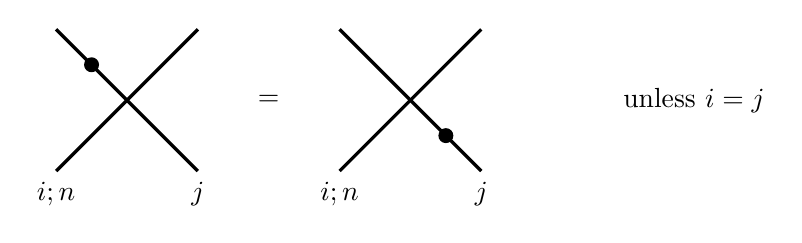
\begin{tikzpicture}[scale=.9,baseline]
      \draw[very thick](-4,0) +(-1,-1) -- +(1,1) node[below,at start]
      {$i;n$}; \draw[very thick](-4,0) +(1,-1) -- +(-1,1) node[below,at
      start] {$j$}; \fill (-4.5,.5) circle (3pt);
      % \draw[very thick] (0,0) +(0,-1) -- +(0,1) node[below, at
      % start]{$i$}; \fill (0,0) circle (5pt);
      \node at (-2,0){=}; \draw[very thick](0,0) +(-1,-1) -- +(1,1)
      node[below,at start] {$i;n$}; \draw[very thick](0,0) +(1,-1) --
      +(-1,1) node[below,at start] {$j$}; \fill (.5,-.5) circle (3pt);
      \node at (4,0){unless $i=j$};
    \end{tikzpicture}
  \end{equation*}
\begin{equation*}\subeqn\label{b-second-QH}
    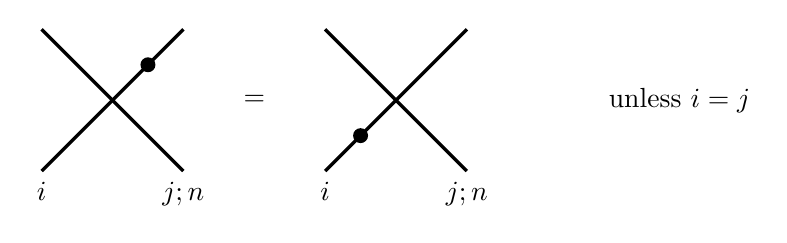
\begin{tikzpicture}[scale=.9,baseline]
      \draw[very thick](-4,0) +(-1,-1) -- +(1,1) node[below,at start]
      {$i$}; \draw[very thick](-4,0) +(1,-1) -- +(-1,1) node[below,at
      start] {$j;n$}; \fill (-3.5,.5) circle (3pt);
      % \draw[very thick] (0,0) +(0,-1) -- +(0,1) node[below, at
      % start]{$i$}; \fill (0,0) circle (5pt);
      \node at (-2,0){=}; \draw[very thick](0,0) +(-1,-1) -- +(1,1)
      node[below,at start] {$i$}; \draw[very thick](0,0) +(1,-1) --
      +(-1,1) node[below,at start] {$j;n$}; \fill (-.5,-.5) circle (3pt);
      \node at (4,0){unless $i=j$};
    \end{tikzpicture}
  \end{equation*}
  \begin{equation*}\subeqn\label{b-third-QH}
    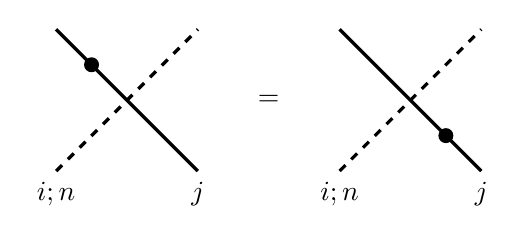
\begin{tikzpicture}[scale=.9,baseline]
      \draw[very thick,dashed](-4,0) +(-1,-1) -- +(1,1) node[below,at start]
      {$i;n$}; \draw[very thick](-4,0) +(1,-1) -- +(-1,1) node[below,at
      start] {$j$}; \fill (-4.5,.5) circle (3pt);
      % \draw[very thick] (0,0) +(0,-1) -- +(0,1) node[below, at
      % start]{$i$}; \fill (0,0) circle (5pt);
      \node at (-2,0){=}; \draw[very thick,dashed](0,0) +(-1,-1) -- +(1,1)
      node[below,at start] {$i;n$}; \draw[very thick](0,0) +(1,-1) --
      +(-1,1) node[below,at start] {$j$}; \fill (.5,-.5) circle (3pt);
    \end{tikzpicture}\qquad \qquad
    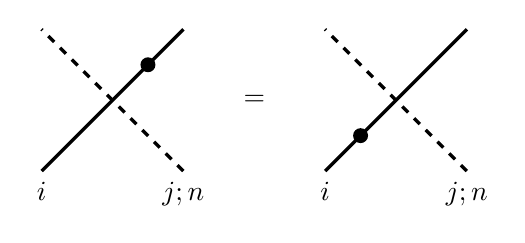
\begin{tikzpicture}[scale=.9,baseline]
      \draw[very thick](-4,0) +(-1,-1) -- +(1,1) node[below,at start]
      {$i$}; \draw[very thick,dashed](-4,0) +(1,-1) -- +(-1,1) node[below,at
      start] {$j;n$}; \fill (-3.5,.5) circle (3pt);
      % \draw[very thick] (0,0) +(0,-1) -- +(0,1) node[below, at
      % start]{$i$}; \fill (0,0) circle (5pt);
      \node at (-2,0){=}; \draw[very thick](0,0) +(-1,-1) -- +(1,1)
      node[below,at start] {$i$}; \draw[very thick,dashed](0,0) +(1,-1) --
      +(-1,1) node[below,at start] {$j;n$}; \fill (-.5,-.5) circle (3pt);
    \end{tikzpicture}
  \end{equation*}
The flavor $\phi$ acts by automorphisms of the $\gls{G}$-representation on $V$,
and thus is induced by a cocharacter into $\prod_iGL(\C^{\glslink{Bw}{w_i}})
\times\prod_{(i,j)\in {\vertex}^2} GL(\C^{\chi_{i,j}})$.  We can
assume that this cocharacter lands in the usual torus of diagonal
matrices; let $c_{i,1},\dots, c_{i,\glslink{Bw}{w_i}}$ be the weights
of its components into
$GL(\C^{\glslink{Bw}{w_i}})$ and $b_e$ for each edge $e$ the weights
of its components into $GL(\C^{\chi_{i,j}})$.
  Let
  \begin{align*}
\subeqn   \label{eq:p-def} p_{i}(u)&=\prod_{k=1}^{\glslink{Bw}{w_i}}(u-c_{i,k}-\frac{h}{2})\\
\subeqn   \label{eq:q-def} q_{ij}(u)&=\prod_{e\colon  j\to i} (u+b_e+\frac{h}{2})\cdot \prod_{e\colon
      i\to j}  (-u+b_e+\frac{h}{2}).
  \end{align*}


  This is the point where we must incorporate that our path is shifted
  by $\phi$.  Thus, when we use the relation 
  (\ref{eq:wall-cross1}) implies to switch the order of
  crossings on disjoint strands, we have:
   \begin{equation*}\subeqn\label{x-cost-1}
  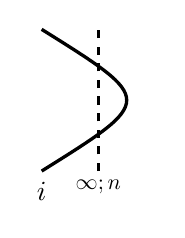
\begin{tikzpicture}[very thick,baseline,scale=.9]
    \draw (-2.8,0)  +(0,-1) .. controls (-1.2,0) ..  +(0,1) node[below,at start]{$i$};
       \draw[dashed] (-2,0)  +(0,-1)--node[below,at start,scale=.8]{$\infty;n$}  +(0,1);
  \end{tikzpicture}
=   p_{i}\Bigg(
  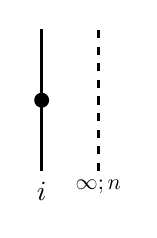
\begin{tikzpicture}[very thick,baseline,scale=.9]
 \draw[dashed] (2.3,0)  +(0,-1) -- node[below,at start,scale=.8]{$\infty;n$} +(0,1);
       \draw (1.5,0)  +(0,-1) -- +(0,1) node[below,at start]{$i$};
       \fill (1.5,0) circle (3pt);
\end{tikzpicture}-nh 
  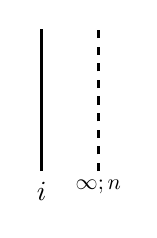
\begin{tikzpicture}[very thick,baseline,scale=.9] \draw[dashed] (2.3,0)  +(0,-1) -- node[below,at start,scale=.8]{$\infty;n$} +(0,1);
       \draw (1.5,0)  +(0,-1) -- +(0,1) node[below,at start]{$i$};
\end{tikzpicture}\Bigg)
\end{equation*}\begin{equation*}
    \subeqn\label{x-cost-2}
  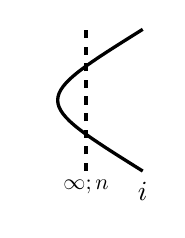
\begin{tikzpicture}[very thick,baseline,scale=.9]
          \draw[dashed] (-2,0)  +(0,-1)-- node[below,at start,scale=.8]{$\infty;n$} +(0,1);
  \draw (-1.2,0)  +(0,-1) .. controls (-2.8,0) ..  +(0,1) node[below,at start]{$i$};\end{tikzpicture}
           =p_{i}\Bigg(
  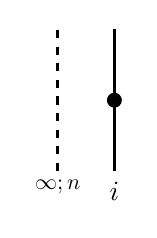
\begin{tikzpicture}[very thick,baseline,scale=.9]
    \draw (2.5,0)  +(0,-1) -- +(0,1) node[below,at start]{$i$};
       \draw[dashed] (1.7,0)  +(0,-1) -- node[below,at start,scale=.8]{$\infty;n$} +(0,1) ;
       \fill (2.5,0) circle (3pt);\end{tikzpicture}- nh  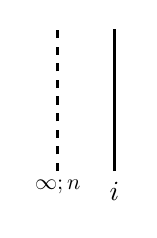
\begin{tikzpicture}[very thick,baseline,scale=.9]
    \draw (2.5,0)  +(0,-1) -- +(0,1) node[below,at start]{$i$};
       \draw[dashed] (1.7,0)  +(0,-1) -- node[below,at start,scale=.8]{$\infty;n$} +(0,1) ;
      \end{tikzpicture} \Bigg)
    \end{equation*}
   \begin{equation*}\subeqn\label{b-black-bigon1}
      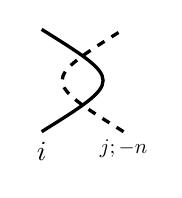
\begin{tikzpicture}[very thick,scale=.65,baseline]
      \draw(-2.8,0) +(0,-1) .. controls (-1.2,0) ..  +(0,1)
      node[below,at start]{$i$}; \draw[dashed] (-1.2,0) +(0,-1) .. controls
(-2.8,0) ..  +(0,1) node[below,at start,scale=.75]{$j;-n$};
\end{tikzpicture}\quad   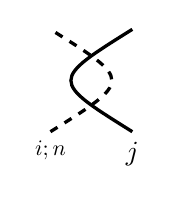
\begin{tikzpicture}[very thick,scale=.65,baseline]
      \draw[dashed] (-2.8,0) +(0,-1) .. controls (-1.2,0) ..  +(0,1)
      node[below,at start,scale=.8]{$i;n$}; \draw (-1.2,0) +(0,-1) .. controls
(-2.8,0) ..  +(0,1) node[below,at start]{$j$};
\end{tikzpicture}
=q_{ij}\Bigg(    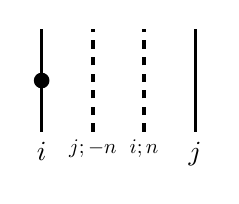
\begin{tikzpicture}[very thick,scale=.65,baseline]
      \draw(-2.8,0) +(0,-1) -- node[midway,fill=black, inner sep=2pt, circle]{} +(0,1)
      node[below,at start]{$i$}; \draw[dashed] (-1.8,0) +(0,-1) -- +(0,1) node[below,at start,scale=.75]{$j;-n$};
      \draw[dashed] (-.8,0) +(0,-1)-- +(0,1)
      node[below,at start,scale=.75]{$i;n$}; \draw (.2,0) +(0,-1) --+(0,1) node[below,at start]{$j$};
\end{tikzpicture}-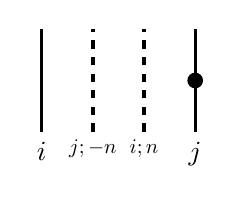
\begin{tikzpicture}[very thick,scale=.65,baseline]
      \draw(-2.8,0) +(0,-1) -- +(0,1)
      node[below,at start]{$i$}; \draw[dashed] (-1.8,0) +(0,-1) -- +(0,1) node[below,at start,scale=.75]{$j;-n$};
      \draw[dashed] (-.8,0) +(0,-1)-- +(0,1)
      node[below,at start,scale=.75]{$i;n$}; \draw (.2,0) +(0,-1) --node[midway,fill=black, inner sep=2pt, circle]{}+(0,1) node[below,at start]{$j$};
\end{tikzpicture}-nh  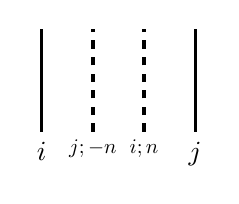
\begin{tikzpicture}[very thick,scale=.65,baseline]
      \draw(-2.8,0) +(0,-1) -- +(0,1)
      node[below,at start]{$i$}; \draw[dashed] (-1.8,0) +(0,-1) -- +(0,1) node[below,at start,scale=.75]{$j;-n$};
      \draw[dashed] (-.8,0) +(0,-1)-- +(0,1)
      node[below,at start,scale=.75]{$i;n$}; \draw (.2,0) +(0,-1) --+(0,1) node[below,at start]{$j$};
\end{tikzpicture}\Bigg)
\end{equation*}
   \begin{equation*}\subeqn\label{b-black-bigon2}
      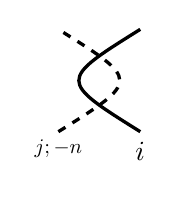
\begin{tikzpicture}[very thick,scale=.65,baseline]
      \draw (-1.2,0) +(0,-1) .. controls
(-2.8,0) ..  +(0,1) node[below,at start]{$i$};
\draw[dashed] (-2.8,0) +(0,-1) .. controls (-1.2,0) ..  +(0,1) node[below,at start,scale=.75]{$j;-n$};
\end{tikzpicture}\quad   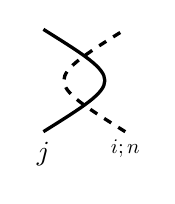
\begin{tikzpicture}[very thick,scale=.65,baseline]
      \draw[dashed] (-1.2,0) +(0,-1) .. controls
(-2.8,0) ..  +(0,1) 
      node[below,at start,scale=.75]{$i;n$}; \draw (-2.8,0) +(0,-1) .. controls (-1.2,0) ..  +(0,1) node[below,at start]{$j$};
\end{tikzpicture}
=q_{ij}\Bigg(    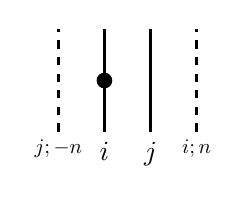
\begin{tikzpicture}[very thick,scale=.65,baseline,xscale=.9]
      \draw(-1.8,0) +(0,-1) -- node[midway,fill=black, inner sep=2pt, circle]{} +(0,1)
      node[below,at start]{$i$}; \draw[dashed] (-2.8,0) +(0,-1) -- +(0,1) node[below,at start,scale=.75]{$j;-n$};
      \draw[dashed] (.2,0) +(0,-1)-- +(0,1)
      node[below,at start,scale=.75]{$i;n$}; \draw (-.8,0) +(0,-1) --+(0,1) node[below,at start]{$j$};
\end{tikzpicture}-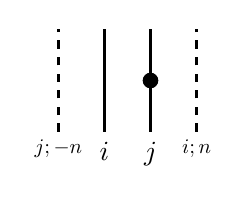
\begin{tikzpicture}[very thick,scale=.65,baseline,xscale=.9]
      \draw(-1.8,0) +(0,-1) -- +(0,1)
      node[below,at start]{$i$}; \draw[dashed] (-2.8,0) +(0,-1) -- +(0,1) node[below,at start,scale=.75]{$j;-n$};
      \draw[dashed](.2,0) +(0,-1)-- +(0,1)
      node[below,at start,scale=.75]{$i;n$}; \draw  (-.8,0)+(0,-1) --node[midway,fill=black, inner sep=2pt, circle]{}+(0,1) node[below,at start]{$j$};
\end{tikzpicture}-n h 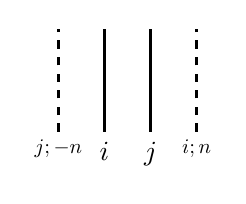
\begin{tikzpicture}[very thick,scale=.65,baseline,xscale=.9]
      \draw(-1.8,0) +(0,-1) -- +(0,1)
      node[below,at start]{$i$}; \draw[dashed] (-2.8,0) +(0,-1) -- +(0,1) node[below,at start,scale=.75]{$j;-n$};
      \draw[dashed] (.2,0) +(0,-1)-- +(0,1)
      node[below,at start,scale=.75]{$i;n$}; \draw  (-.8,0) +(0,-1) --+(0,1) node[below,at start]{$j$};
\end{tikzpicture}\Bigg)
  \end{equation*}
Note that the equations above are written assuming that $n>0$ (and
implicitly $n\in \Z-\frac{1}{2}$), but they are equally valid if $n<0$,
with the requisite reordering of strands.
The relation 
(\ref{eq:psi2}) implies that:
  \begin{equation*}\subeqn\label{b-psi2}
    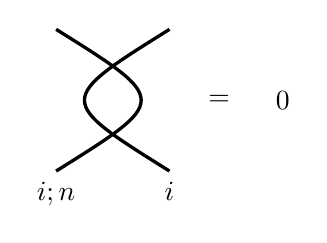
\begin{tikzpicture}[very thick,scale=.9,baseline]
      \draw (-2.8,0) +(0,-1) .. controls (-1.2,0) ..  +(0,1)
      node[below,at start]{$i;n$}; \draw (-1.2,0) +(0,-1) .. controls
      (-2.8,0) ..  +(0,1) node[below,at start]{$i$}; \node at (-.5,0)
      {=}; \node at (0.4,0) {$0$};
    \end{tikzpicture}\qquad \qquad    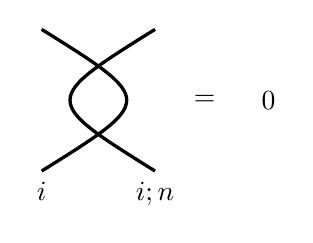
\begin{tikzpicture}[very thick,scale=.9,baseline]
      \draw (-2.8,0) +(0,-1) .. controls (-1.2,0) ..  +(0,1)
      node[below,at start]{$i$}; \draw(-1.2,0) +(0,-1) .. controls
      (-2.8,0) ..  +(0,1) node[below,at start]{$i;n$}; \node at (-.5,0)
      {=}; \node at (0.4,0) {$0$};
    \end{tikzpicture}
      \end{equation*}
The relation 
(\ref{eq:psipoly}) is equivalent to isotopy and  \begin{equation*}\subeqn\label{b-nilHecke-1}
    \begin{tikzpicture}[scale=.9,baseline]
      \draw[very thick](-4,0) +(-1,-1) -- +(1,1) node[below,at start,scale=.8]
      {$i;n$}; \draw[very thick](-4,0) +(1,-1) -- +(-1,1) node[below,at
      start] {$i$}; \fill (-4.5,.5) circle (3pt);
      % \draw[very thick] (0,0) +(0,-1) -- +(0,1) node[below, at
      % start]{$i$}; \fill (0,0) circle (5pt);
      \node at (-2,0){$-$}; \draw[very thick](0,0) +(-1,-1) -- +(1,1)
      node[below,at start,scale=.8]
      {$i;n$}; \draw[very thick](0,0) +(1,-1) --
      +(-1,1) node[below,at start] {$i$}; \fill (.5,-.5) circle (3pt);
     \node at (2,0){$=$};  \draw[very thick](4,0) +(-1,-1) -- +(-1,1)
      node[below,at start,scale=.8]
      {$i;n$}; \draw[very thick](4,0) +(0,-1) --
      +(0,1) node[below,at start] {$i$};
      \draw[weyl] (4,0) +(.5,0) -- +(-1.5,0) node[at start, right,green!50!black]{$s$} ;
    \end{tikzpicture}
  \end{equation*}
 \begin{equation*}\subeqn\label{b-nilHecke-2}
    \begin{tikzpicture}[scale=.9,baseline]
      \draw[very thick](-4,0) +(-1,-1) -- +(1,1) node[below,at
      start] {$i$}; \draw[very thick](-4,0) +(1,-1) -- +(-1,1) node[below,at start,scale=.8]
      {$i;n$}; \fill (-4.5,-.5) circle (3pt);
      % \draw[very thick] (0,0) +(0,-1) -- +(0,1) node[below, at
      % start]{$i$}; \fill (0,0) circle (5pt);
      \node at (-2,0){$-$}; \draw[very thick](0,0) +(-1,-1) -- +(1,1)
      node[below,at
      start] {$i$}; \draw[very thick](0,0) +(1,-1) --
      +(-1,1) node[below,at start,scale=.8]
      {$i;n$}; \fill (.5,.5) circle (3pt);
      \node at (2,0){$=$};  \draw[very thick](4,0) +(-1,-1) -- +(-1,1)
      node[below,at
      start] {$i$}; \draw[very thick](4,0) +(0,-1) --
      +(0,1) node[below,at start,scale=.8]
      {$i;n$}; 
      \draw[weyl] (4,0) +(.5,0) -- +(-1.5,0) node[at start, right,green!50!black]{$s$} ;
    \end{tikzpicture}
  \end{equation*}
  with $s$ denoting the unique reflection in the affine Weyl group
  switching the top and bottom labels of the diagram.

  Finally, the codimension 2 relations show how to relate the two
resolutions of a triple point. The correct relation depends on the
number of partners with the same label going through the triple
point: if all three, then we use (\ref{eq:psi}), if two we use
(\ref{eq:triple}) and if there is no such pair, then
(\ref{eq:wall-cross1}).  \excise{ Any triple point involving only partners
  \begin{equation*}\subeqn\label{b-triple-coxeter}
      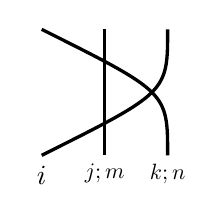
\begin{tikzpicture}[very thick,scale=.8,baseline]  \draw (1,0) +(1,-1) .. controls
      (2,0) .. +(-1,1)
      node[below,at start,scale=.8]{$k;n$}; \draw (1,0) +(-1,-1) .. controls
      (2,0) .. +(1,1)
      node[below,at start]{$i$}; \draw (1,0) +(0,-1) -- node[below, at start,scale=.8]{$j;m$}+(0,1); 
    \end{tikzpicture} =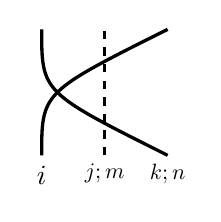
\begin{tikzpicture}[very thick,scale=.8,baseline]
      \draw (-3,0) +(1,-1) .. controls (-4,0) .. +(-1,1) node[below,at start,scale=.8]{$k;n$}; \draw
      (-3,0) +(-1,-1) .. controls (-4,0) .. +(1,1) node[below,at start]{$i$}; \draw[dashed]
      (-3,0) +(0,-1)--  node[below, at start,scale=.8]{$j;m$}+(0,1);
       \end{tikzpicture} 
  \end{equation*}
 
  Finally, the codimension 2 relation
 (\ref{eq:triple}) implies a number of different relations relating the
 two different ways of resolving a triple point
 for all 
 ghosts, we have the equation below and its reflection through a
 vertical line:
  \begin{equation*}\subeqn\label{b-triple-extra-dumb}
    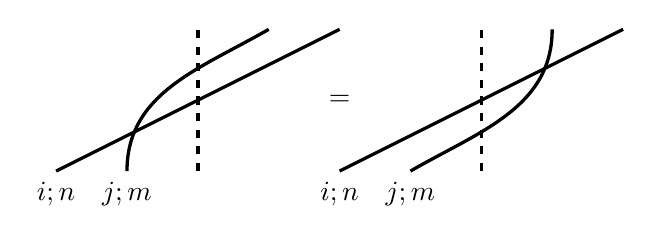
\begin{tikzpicture}[very thick,scale=.9,baseline]
      \draw (-3,0) +(-1,-1) to[out=90,in=-150] node[below,at start]{$j;m$} +(1,1) ; \draw
      (-3,0) +(-2,-1) -- +(2,1) node[below,at start]{$i;n$}; \draw[dashed]
      (-3,0) +(0,-1)--  +(0,1); \node at (-1,0) {=}; \draw (1,0) +(-1,-1) to [out=30,in=-90] node[below,at start]{$j;m$} +(1,1)
      ; \draw
      (1,0) +(-2,-1) -- +(2,1) node[below,at start]{$i;n$}; \draw[dashed] (1,0) +(0,-1) -- +(0,1); 
    \end{tikzpicture}
  \end{equation*}}
These imply we can isotope through any triple point unless it involves
exactly two partners with the label $i\in {\gls{vertex}}$.  In order to
cover this last case, let
  \begin{align*}
\partial_{m }p(u_1,u_2)&=\frac{p(u_1-mh)-p(u_2-mh)}{u_1-u_2}\\ \partial_{n,m}q(u_1,v,u_2)&=\frac{q(u_1-v+mh)-q(u_2-v+mh)}{u_1-u_2}
  \end{align*}

  \begin{equation*}\subeqn\label{b-frame-triple-smart}
      \begin{tikzpicture}[very thick,scale=.8,baseline]  \draw (1,0) +(1,-1) .. controls
      (2,0) .. +(-1,1)
      node[below,at start,scale=.8]{$i;n$}; \draw (1,0) +(-1,-1) .. controls
      (2,0) .. +(1,1)
      node[below,at start]{$i$}; \draw[dashed] (1,0) +(0,-1) -- node[above, at end,scale=.8]{$\infty;m$}+(0,1);  \draw[weyl] (1,.7) +(1.5,0) -- +(-1.5,0) node[at start, right]{$s$} ;
    \end{tikzpicture} - \begin{tikzpicture}[very thick,scale=.8,baseline]
      \draw (-3,0) +(1,-1) .. controls (-4,0) .. +(-1,1) node[below,at start,scale=.8]{$i;n$}; \draw
      (-3,0) +(-1,-1) .. controls (-4,0) .. +(1,1) node[below,at start]{$i$}; \draw[dashed]
      (-3,0) +(0,-1)--  node[above, at end,scale=.8]{$\infty;m$}+(0,1);  \draw[weyl] (-3,.7) +(1.5,0) -- +(-1.5,0) node[at start, right]{$s$} ;
       \end{tikzpicture} 
  =\partial_{n}p_i\Bigg(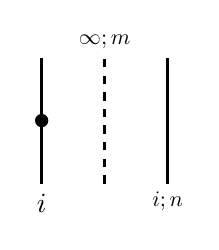
\begin{tikzpicture}[very thick,scale=.8,baseline]       \draw (0,0)
      +(1,-1) -- +(1,1) node[below,at start,scale=.8]{$i;n$};  \fill (-1,0) circle (3pt);\draw (0,0)
      +(-1,-1) -- +(-1,1) node[below,at start]{$i$}; \draw[dashed] (0,0)
      +(0,-1) -- node[above, at end,scale=.8]{$\infty;m$}+(0,1); 
    \end{tikzpicture}, 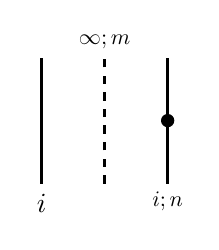
\begin{tikzpicture}[very thick,scale=.8,baseline]       \draw (0,0)
      +(1,-1) -- +(1,1) node[below,at start,scale=.8]{$i;n$};  \fill (1,0) circle (3pt);\draw (0,0)
      +(-1,-1) -- +(-1,1) node[below,at start]{$i$}; \draw[dashed] (0,0)
      +(0,-1) -- node[above, at end,scale=.8]{$\infty;m$}+(0,1);
    \end{tikzpicture}\Bigg)
  \end{equation*}
   \begin{equation*}
       \subeqn\label{b-triple-smart}
      \begin{tikzpicture}[very thick,scale=.7,baseline,xscale=.9]  \draw (1,0) +(1,-1) .. controls
      (2,0) .. +(-1,1)
      node[below,at start,scale=.8]{$i;n$}; \draw (1,0) +(-1,-1) .. controls
      (2,0) .. +(1,1)
      node[below,at start]{$i$}; \draw[dashed] (1,0) +(0,-1) -- node[above, at end,scale=.8]{$j;m$}+(0,1);  \draw[dashed] (5,0) +(1,-1) .. controls
      (6,0) .. +(-1,1)
      node[above,at end,scale=.8]{$i;\!-m$}; \draw[dashed] (5,0) +(-1,-1) .. controls
      (6,0) .. +(1,1)
      node[above,at end,scale=.8]{$i;n\!-\!m$}; \draw (5,0) +(0,-1) -- node[below, at start]{$j$}+(0,1);  \draw[weyl] (5,.4) +(1.5,0) -- +(-5.5,0) node[at start, right]{$s$} ;
    \end{tikzpicture}  
    %\begin{tikzpicture}[very thick,scale=.7,baseline,xscale=.9]  \draw (1,0) +(1,-1) .. controls
    %  (2,0) .. +(-1,1)
    %  node[below,at start]{$i$}; \draw (1,0) +(-1,-1) .. controls
    %  (2,0) .. +(1,1)
    %  node[below,at start,scale=.8]{$i;\!-n$}; \draw[dashed] (1,0) +(0,-1) -- node[above, at end,scale=.8]{$j;m\!-\!n$}+(0,1); 
    %\end{tikzpicture}   
    - \begin{tikzpicture}[very thick,scale=.7,baseline,xscale=.9]
      \draw (-3,0) +(1,-1) .. controls (-4,0) .. +(-1,1) node[below,at start,scale=.8]{$i;n$}; \draw
      (-3,0) +(-1,-1) .. controls (-4,0) .. +(1,1) node[below,at start]{$i$}; \draw[dashed]
      (-3,0) +(0,-1)--  node[above, at end,scale=.8]{$j;m$}+(0,1);  
      \draw[dashed] (1,0) +(1,-1) .. controls (0,0) .. +(-1,1) node[above,at end,scale=.8]{$i;\!-m$}; \draw[dashed]
      (1,0) +(-1,-1) .. controls (0,0) .. +(1,1) node[above,at end,scale=.8]{$i;n\!-\!m$}; \draw
      (1,0) +(0,-1)--  node[below, at start]{$j$}+(0,1);  \draw[weyl] (-1,.4) +(3.5,0) -- +(-3.5,0) node[at start, right]{$s$} ;
       \end{tikzpicture} 
       %\begin{tikzpicture}[very thick,scale=.7,baseline,xscale=.9]
      %\draw (-3,0) +(1,-1) .. controls (-4,0) .. +(-1,1) %node[below,at start,scale=.8]{$i;n$}; \draw
      %(-3,0) +(-1,-1) .. controls (-4,0) .. +(1,1) node[below,at %start,scale=.8]{$i;\!-n$}; \draw[dashed]
      %(-3,0) +(0,-1)--  node[above, at %end,scale=.8]{$j;m\!-\!n$}+(0,1);
       %\end{tikzpicture} 
  =\partial_{n,m}q_{ij}(\gamma_1, \gamma_2, \gamma_3)
\end{equation*}
\begin{equation*}
 \gamma_1=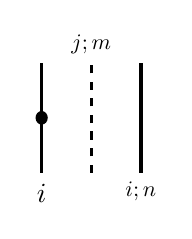
\begin{tikzpicture}[very thick,scale=.7,baseline,xscale=.9]       \draw (0,0)
      +(1,-1) -- +(1,1) node[below,at start,scale=.8]{$i;n$};  \fill (-1,0) circle (3.5pt);\draw (0,0)
      +(-1,-1) -- +(-1,1) node[below,at start]{$i$}; \draw[dashed] (0,0)
      +(0,-1) -- node[above, at end,scale=.8]{$j;m$}+(0,1); 
    \end{tikzpicture} 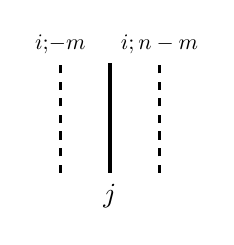
\begin{tikzpicture}[very
      thick,scale=.7,baseline,xscale=.9]  \draw[dashed] (1,0) +(1,-1) -- +(1,1)
      node[above,at end,scale=.8]{$i;n-m$}; \draw[dashed] (1,0) +(-1,-1) --+(-1,1)
      node[above,at end,scale=.8]{$i;\!-m$}; \draw (1,0) +(0,-1) -- node[below, at start]{$j$}+(0,1); 
    \end{tikzpicture}
    %\begin{tikzpicture}[very thick,scale=.7,baseline,xscale=.9]    %   \draw (0,0)
    %  +(1,-1) -- +(1,1) node[below,at start]{$i$}; \draw (0,0)
%      +(-1,-1) -- +(-1,1) node[below,at start,scale=.8]{$i;\!-n$}; \draw[dashed] (0,0)
 %     +(0,-1) -- node[above, at end,scale=.8]{$j;m\!-\!n$}+(0,1); 
    %\end{tikzpicture}  
    \quad  \gamma_2= \begin{tikzpicture}[very thick,scale=.7,baseline,xscale=.9]       \draw (0,0)
      +(1,-1) -- +(1,1) node[below,at start,scale=.8]{$i;n$};  \draw (0,0)
      +(-1,-1) -- +(-1,1) node[below,at start]{$i$}; \draw[dashed] (0,0)
      +(0,-1) -- node[above, at end,scale=.8]{$j;m$}+(0,1); 
    \end{tikzpicture}\begin{tikzpicture}[very
      thick,scale=.7,baseline,xscale=.9]  \draw[dashed] (1,0) +(1,-1) -- +(1,1)
      node[above,at end,scale=.8]{$i;n-m$}; \draw[dashed] (1,0) +(-1,-1) --+(-1,1)
      node[above,at end,scale=.8]{$i;\!-m$}; \draw (1,0) +(0,-1) -- node[below, at start]{$j$}+(0,1); \fill (1,0) circle (3.5pt);
    \end{tikzpicture}
   % \begin{tikzpicture}[very thick,scale=.7,baseline,xscale=.9]     %  \draw (0,0)
    %  +(1,-1) -- +(1,1) node[below,at start]{$i$}; \draw (0,0)
    %  +(-1,-1) -- +(-1,1) node[below,at start,scale=.8]{$i;\!-n$}; %\draw[dashed] (0,0)
    %  +(0,-1) -- node[above, at end,scale=.8]{$j;m\!-\!n$}+(0,1); 
%    \end{tikzpicture} 
  %  \end{equation*}
%\begin{equation*} 
\quad
\gamma_3= \begin{tikzpicture}[very thick,scale=.7,baseline,xscale=.9]       \draw (0,0)
      +(1,-1) -- +(1,1) node[below,at start,scale=.8]{$i;n$};  \draw (0,0)
      +(-1,-1) -- +(-1,1) node[below,at start]{$i$}; \draw[dashed] (0,0)
      +(0,-1) -- node[above, at end,scale=.8]{$j;m$}+(0,1);       \fill (1,0) circle (3.5pt);
    \end{tikzpicture}\begin{tikzpicture}[very
      thick,scale=.7,baseline,xscale=.9]  \draw[dashed] (1,0) +(1,-1) -- +(1,1)
      node[above,at end,scale=.8]{$i;n-m$}; \draw[dashed] (1,0) +(-1,-1) --+(-1,1)
      node[above,at end,scale=.8]{$i;\!-m$}; \draw (1,0) +(0,-1) -- node[below, at start]{$j$}+(0,1); 
    \end{tikzpicture}
    %\begin{tikzpicture}[very thick,scale=.7,baseline,xscale=.9]       \draw (0,0)
    %  +(1,-1) -- +(1,1) node[below,at start]{$i$}; \draw (0,0)
    %  +(-1,-1) -- +(-1,1) node[below,at start,scale=.8]{$i;\!-n$}; %\draw[dashed] (0,0)
    %  +(0,-1) -- node[above, at end,scale=.8]{$j;m\!-\!n$}+(0,1); 
%    \end{tikzpicture} 
  \end{equation*}
  with $s$ denoting the unique reflection in the affine Weyl group
  making the top and bottom match.  As before, using $p$ and $q$
  accounts for our shift by $\gls{flav}$.

  Given this reinterpretation of our relations in terms of diagrams, this allows us to interpret the relations (\ref{eq:dot-migration}--\ref{b-triple-smart}) as relations on unrolled diagrams, by setting $\sum a_iD_i=0$ if we have that $\sum a_i\mathbbm{r}_{D_i}=0$.
  In this case, we have that:
  \begin{lemma}\label{lem:unrolled-B}
    Given $\eta,\eta'\in \ft_{\second}$, the Hom space
    $\Hom_{\gls{scrB}}(\eta,\eta')$ is spanned by the morphisms
    $\mathbbm{r}_D$ for unrolled diagrams $D$ with top $\eta'$ and
    bottom $\eta$, modulo the local relations (\ref{eq:dot-migration}--\ref{b-triple-smart}).
  \end{lemma}
  \begin{proof}
    We have justified in each individual case why the relations
    (\ref{eq:dot-migration}--\ref{b-triple-smart}) hold.  Thus, we have a
    map from the formal span of unrolled diagrams modulo these
    relations to $\Hom_{\mathscr{B}}(\eta,\eta')$.  This is surjective
    because the generating morphisms of the category $\mathscr{B}$ are
    given by the basic unrolled diagrams in
    \eqref{eq:unrolled-possible}.  On the other hand, the relations
    (\ref{eq:dot-migration}--\ref{b-triple-smart}) suffice to write any
     $\mathbbm{r}_D$ as a sum of diagrams corresponding to a reduced word in
    $\widehat{W}$ with all dots and green lines at the bottom, and to
    relate any two reduced words for $w\in \widehat{W}$ modulo the
    diagrams for shorter elements of $\widehat{W}$.  Thus, we find
    that the unrolled diagrams corresponding to the basis of
    \cite[Cor. 3.12]{WebSD} are a spanning set of this quotient.  This
    is only possible if the map is injective as well.
  \end{proof}
  
\subsection{Antipodal diagrams}
\label{sec:antipodal-diagrams}

  The reader may have noticed that these diagrams are actually quite
  difficult to draw and interpret, but there is a symmetry that we
  have not exploited, the action of the extended affine Weyl group.
  The quotient of $\prod_i\R^{\glslink{Bv}{v_i}}$ by the extended Weyl group is
  given by the space $\prod_i (\R/\Z)^{v_i}/S_{v_i}$, which we can
  interpret as the moduli space of multisubsets of the circle $\R/\Z$
  labeled with elements of ${\gls{vertex}}$, such that $v_i$ elements have label $i\in {\vertex}$.
  Thus the path $[0,1]\to \prod_i\R^{v_i}$ composed
  with the projection $\prod_i\R^{v_i}\to \prod_i
  (\R/\Z)^{v_i}/S_{v_i}$ can be thought of as a path in 
  this moduli space.

  We draw this by considering our diagrams in $\R\times [0,1]$, and
  considering the quotient of this plane by $\Z$ acting by addition to
  the $x$-coordinate.  Note that this sends all the partners to
  a single curve in  $\R/\Z\times [0,1]$, and all  ghosts
  to a single curve $\frac{1}{2}$ units in either direction (since we
  are on a circle).  We can describe the
  resulting diagrams as follows:

 \begin{definition}\label{def:cyl-BFN}
  An {\bf antipodal diagram} is a collection of finitely many
  oriented curves in $\R/\Z\times [0,1]$ of the form
  $\{(\bar{\pi}(t),t)\mid t\in [0,1]\}$ for some path $\bar{\pi}\colon
  [0,1]\to \R/\Z$.
  Each curve is labeled with an element $i\in {\gls{vertex}}$ and decorated with
  finitely many dots.  For each curve, we draw a ``ghost'' curve at
  $\{(\bar{\pi}(t)-\frac{1}{2},t)\mid t\in [0,1]\}$, as well as one at
  $\{(-\frac{1}{2},t)\mid t\in [0,1]\}$. 
  We draw these as dashed.

  The diagram must be locally of the
  form given in \eqref{eq:unrolled-possible}.
That is, there are no tangencies, triple crossings or dots on
crossings.  The curves (including ghosts) must
meet the circles at
$y=0$ and $y=1$ at distinct points. We consider these
diagrams 
up to isotopy preserving the conditions above.  
\end{definition}

We call a subset of $\R/\Z$ {\bf generic} if the distance between no pair of elements is $\frac{1}{2}$.  Our conditions above guarantee that for a fixed $t$, the elements $\bar{\pi}(t)$ for the different strands are distinct and form a generic subset if and only if no pair of strands or strand and ghost cross at height $t$.

Every antipodal diagram has a unique lift to a path $[0,1]\to \ft_{\tau}$ which starts in the fundamental region of $\widehat{W}$ where the coordinates $z_{i,k}$ satisfy
\begin{equation}
    -\frac{1}{2}< z_{i,1}<z_{i,2}<\cdots < z_{i,\glslink{Bv}{v_i}}<\frac{1}{2}.  
\end{equation}
That is, by the path lifting property of the universal cover, each of the curves $\bar{\pi}\colon [0,1]\to \R/\Z$ has a unique lift $\pi$ with $-\frac{1}{2}<\pi(0)<\frac{1}{2}$, and we can number these so that \begin{equation}
    -\frac{1}{2}<\pi_{i,1}(0)<\cdots <\pi_{i,v_i}(0)<\frac{1}{2}.
\end{equation} 
\begin{definition}\label{def:antipodal-r}
 Given an antipodal diagram $D$ with no dots, let $\mathbbm{r}_D$ be the morphism defined by the lifted path starting in the fundamental region, followed by the unique element of $\widehat{W}$ sending us back to the fundamental region.    
 
 If the diagram does contain dots, then place these in the lifted diagram on the unique partner preimage which has $x$-value in $(-\frac{1}{2}, \frac{1}{2} )$.
\end{definition}
We have to be careful about lifting antipodal diagrams with dots,
because if we do so in the most naive way, the result will not be
compatible with composition, which the definition above is.  We could accomplish the same effect if instead of 
applying a Weyl group element at the end, we  applied one
immediately whenever we left the fundamental region to move back into
it.  

We can also modify the relations
(\ref{eq:dot-migration}--\ref{b-triple-smart}) to work as relations on
antipodal diagrams, as before following the rule that $\sum a_iD_i=0$
if we have that $\sum a_i\mathbbm{r}_{D_i}=0$.  Some of these can
interpreted locally exactly as they read above:
(\ref{b-first-QH}--\ref{b-second-QH}) and
(\ref{b-psi2}--\ref{b-nilHecke-2}) are of this type. On the other, if
a dot on an antipodal diagram is slid over the half-integer ghost with
label $\infty$, then it goes between lifting to the ghost just right
of $x=-\frac{1}{2}$ to that just left of $x=\frac{1}{2}$.  The effect
of (\ref{eq:dot-migration})  is thus the following relation on antipodal diagrams: \newseq
    \begin{equation*}\subeqn\label{a-dot-slide}
    \begin{tikzpicture}[very thick,baseline,scale=.7]
  \draw(-3,0) +(-1,-1) -- +(1,1);
  \draw[dashed](-3,0) +(0,-1) -- node[below,at start]{$\infty$}  +(0,1);
\fill (-3.5,-.5) circle (3pt); \end{tikzpicture}
=
 \begin{tikzpicture}[very thick,baseline,scale=.7] \draw(1,0) +(-1,-1) -- +(1,1);
  \draw[dashed](1,0) +(0,-1) -- node[below,at start]{$\infty$}  +(0,1);
\fill (1.5,.5) circle (3pt);
    \end{tikzpicture} +h  \begin{tikzpicture}[very thick,baseline,scale=.7] \draw(1,0) +(-1,-1) -- +(1,1);
  \draw[dashed](1,0) +(0,-1) -- node[below,at start]{$\infty$}  +(0,1);
    \end{tikzpicture}
\qquad \qquad     \begin{tikzpicture}[very thick,baseline,scale=.7]
  \draw(-3,0) +(1,-1) -- +(-1,1);
  \draw[dashed](-3,0) +(0,-1) -- node[below,at start]{$\infty$}  +(0,1);
\fill (-2.5,-.5) circle (3pt); \end{tikzpicture}
=
 \begin{tikzpicture}[very thick,baseline,scale=.7] \draw(1,0) +(1,-1) -- +(-1,1);
  \draw[dashed](1,0) +(0,-1) -- node[below,at start]{$\infty$}  +(0,1);
\fill (.5,.5) circle (3pt);
    \end{tikzpicture} -h  \begin{tikzpicture}[very thick,baseline,scale=.7] \draw(1,0) +(1,-1) -- +(-1,1);
  \draw[dashed](1,0) +(0,-1) --node[below,at start]{$\infty$}   +(0,1);
    \end{tikzpicture}
  \end{equation*}
The other relations need to interpreted carefully to be compatible with lifting. For example, the relations (\ref{x-cost-1}--\ref{x-cost-2}) become
  \begin{equation*}\subeqn\label{a-cost-1}
  \begin{tikzpicture}[very thick,baseline,scale=.9]
    \draw (-2.8,0)  +(0,-1) .. controls (-1.2,0) ..  +(0,1) node[below,at start]{$i$};
       \draw[dashed] (-2,0)  +(0,-1)--node[below,at start]{$\infty$}  +(0,1);
  \end{tikzpicture}
=   p_{i}\Bigg(
  \begin{tikzpicture}[very thick,baseline,scale=.9]
 \draw[dashed] (2.3,0)  +(0,-1) -- node[below,at start]{$\infty$} +(0,1);
       \draw (1.5,0)  +(0,-1) -- +(0,1) node[below,at start]{$i$};
       \fill (1.5,0) circle (3pt);
\end{tikzpicture}-\frac{1}{2}h 
  \begin{tikzpicture}[very thick,baseline,scale=.9] \draw[dashed] (2.3,0)  +(0,-1) -- node[below,at start]{$\infty$} +(0,1);
       \draw (1.5,0)  +(0,-1) -- +(0,1) node[below,at start]{$i$};
\end{tikzpicture}\Bigg)
\end{equation*}\begin{equation*}
    \subeqn\label{a-cost-2}
  \begin{tikzpicture}[very thick,baseline,scale=.9]
          \draw[dashed] (-2,0)  +(0,-1)-- node[below,at start]{$\infty$} +(0,1);
  \draw (-1.2,0)  +(0,-1) .. controls (-2.8,0) ..  +(0,1) node[below,at start]{$i$};\end{tikzpicture}
           =p_{i}\Bigg(
  \begin{tikzpicture}[very thick,baseline,scale=.9]
    \draw (2.5,0)  +(0,-1) -- +(0,1) node[below,at start]{$i$};
       \draw[dashed] (1.7,0)  +(0,-1) -- node[below,at start]{$\infty$} +(0,1) ;
       \fill (2.5,0) circle (3pt);\end{tikzpicture}+ \frac{1}{2}h  \begin{tikzpicture}[very thick,baseline,scale=.9]
    \draw (2.5,0)  +(0,-1) -- +(0,1) node[below,at start]{$i$};
       \draw[dashed] (1.7,0)  +(0,-1) -- node[below,at start]{$\infty$} +(0,1) ;
      \end{tikzpicture} \Bigg)
    \end{equation*}
Similarly, the relations (\ref{b-black-bigon1}--\ref{b-black-bigon1}) depend on the cyclic order of the strands $i,j$ and the point $x=-\frac{1}{2}$ on the circle.  Assuming these are cyclically ordered, we have:
  \begin{equation*}\subeqn\label{a-black-bigon1}
      \begin{tikzpicture}[very thick,scale=.65,baseline]
      \draw(-2.8,0) +(0,-1) .. controls (-1.2,0) ..  +(0,1)
      node[below,at start]{$i$}; \draw[dashed] (-1.2,0) +(0,-1) .. controls
(-2.8,0) ..  +(0,1) node[below,at start]{$j$};
\end{tikzpicture}\quad   \begin{tikzpicture}[very thick,scale=.65,baseline]
      \draw[dashed] (-2.8,0) +(0,-1) .. controls (-1.2,0) ..  +(0,1)
      node[below,at start]{$i$}; \draw (-1.2,0) +(0,-1) .. controls
(-2.8,0) ..  +(0,1) node[below,at start]{$j$};
\end{tikzpicture}
=q_{ij}\Bigg(    \begin{tikzpicture}[very thick,scale=.65,baseline]
      \draw(-2.8,0) +(0,-1) -- node[midway,fill=black, inner sep=2pt, circle]{} +(0,1)
      node[below,at start]{$i$}; \draw[dashed] (-1.8,0) +(0,-1) -- +(0,1) node[below,at start]{$j$};
      \draw[dashed] (-.8,0) +(0,-1)-- +(0,1)
      node[below,at start]{$i$}; \draw (.2,0) +(0,-1) --+(0,1) node[below,at start]{$j$};
\end{tikzpicture}-\begin{tikzpicture}[very thick,scale=.65,baseline]
      \draw(-2.8,0) +(0,-1) -- +(0,1)
      node[below,at start]{$i$}; \draw[dashed] (-1.8,0) +(0,-1) -- +(0,1) node[below,at start]{$j$};
      \draw[dashed] (-.8,0) +(0,-1)-- +(0,1)
      node[below,at start]{$i$}; \draw (.2,0) +(0,-1) --node[midway,fill=black, inner sep=2pt, circle]{}+(0,1) node[below,at start]{$j$};
\end{tikzpicture}-\frac{1}{2}h  \begin{tikzpicture}[very thick,scale=.65,baseline]
      \draw(-2.8,0) +(0,-1) -- +(0,1)
      node[below,at start]{$i$}; \draw[dashed] (-1.8,0) +(0,-1) -- +(0,1) node[below,at start]{$j$};
      \draw[dashed] (-.8,0) +(0,-1)-- +(0,1)
      node[below,at start]{$i$}; \draw (.2,0) +(0,-1) --+(0,1) node[below,at start]{$j$};
\end{tikzpicture}\Bigg)
\end{equation*}
   \begin{equation*}\subeqn\label{a-black-bigon2}
      \begin{tikzpicture}[very thick,scale=.65,baseline]
      \draw (-1.2,0) +(0,-1) .. controls
(-2.8,0) ..  +(0,1) node[below,at start]{$i$};
\draw[dashed] (-2.8,0) +(0,-1) .. controls (-1.2,0) ..  +(0,1) node[below,at start]{$j$};
\end{tikzpicture}\quad   \begin{tikzpicture}[very thick,scale=.65,baseline]
      \draw[dashed] (-1.2,0) +(0,-1) .. controls
(-2.8,0) ..  +(0,1) 
      node[below,at start]{$i$}; \draw (-2.8,0) +(0,-1) .. controls (-1.2,0) ..  +(0,1) node[below,at start]{$j$};
\end{tikzpicture}
=q_{ij}\Bigg(    \begin{tikzpicture}[very thick,scale=.65,baseline,xscale=.9]
      \draw(-1.8,0) +(0,-1) -- node[midway,fill=black, inner sep=2pt, circle]{} +(0,1)
      node[below,at start]{$i$}; \draw[dashed] (-2.8,0) +(0,-1) -- +(0,1) node[below,at start]{$j$};
      \draw[dashed] (.2,0) +(0,-1)-- +(0,1)
      node[below,at start]{$i$}; \draw (-.8,0) +(0,-1) --+(0,1) node[below,at start]{$j$};
\end{tikzpicture}-\begin{tikzpicture}[very thick,scale=.65,baseline,xscale=.9]
      \draw(-1.8,0) +(0,-1) -- +(0,1)
      node[below,at start]{$i$}; \draw[dashed] (-2.8,0) +(0,-1) -- +(0,1) node[below,at start]{$j$};
      \draw[dashed](.2,0) +(0,-1)-- +(0,1)
      node[below,at start]{$i$}; \draw  (-.8,0)+(0,-1) --node[midway,fill=black, inner sep=2pt, circle]{}+(0,1) node[below,at start]{$j$};
\end{tikzpicture}-\frac{1}{2} h \begin{tikzpicture}[very thick,scale=.65,baseline,xscale=.9]
      \draw(-1.8,0) +(0,-1) -- +(0,1)
      node[below,at start]{$i$}; \draw[dashed] (-2.8,0) +(0,-1) -- +(0,1) node[below,at start]{$j$};
      \draw[dashed] (.2,0) +(0,-1)-- +(0,1)
      node[below,at start]{$i$}; \draw  (-.8,0) +(0,-1) --+(0,1) node[below,at start]{$j$};
\end{tikzpicture}\Bigg)
  \end{equation*}
Since we can switch $i$ and $j$ without loss of generality, we do not need a second version of these relations.  
\begin{definition}  The {\bf antipodal KLR category}  is the category whose \begin{itemize}
    \item objects are generic subsets  of $\R/\Z$, labeled with elements of ${\gls{vertex}}$, with $\glslink{Bv}{v_i}$ having label $i$.
    \item morphisms are the quotient of the formal span of antipodal diagrams
  over $\K[c_{*,*},b_*]$  modulo the relations induced by (\ref{eq:dot-migration}--\ref{b-triple-smart}), in particular  by (\ref{a-dot-slide}--\ref{a-black-bigon2}).  
\end{itemize}  
% We let the {\bf cylindrical BFN category} be the category whose objects are subsets of $(\R/\Z)\setminus \{0\}$, with each element of the subset labeled with $i\in \gls{quiver}$, and whose morphisms are cylindrical KLR diagrams with the source at bottom and target at top.  
\end{definition}
Some might prefer to think about the antipodal KLR algebra, which is
the endomorphisms of the formal sum of all objects in this category.
Lemma \ref{lem:unrolled-B} can thus be rephrased as:
\begin{proposition}\label{prop:KLR-B}
The antipodal KLR category is equivalent to the category $\gls{scrB}$. 
\end{proposition}
Note, this construction is closely related to the flag Yangian introduced in \cite[Def. 4.12]{KTWWY2}.  In that paper, we assumed that $\gls{quiver} $ was bipartite (with the sets of nodes called {\bf even} and {\bf odd}), 
that if $i\to j$ then $i$ is even and $j$ odd.  Furthermore, the
definition depended on a polynomial $p_i$.  If 
$h=2$, $b_e=0$ and the scalars $c_{i,k}$ are the roots (with
multiplicity) of $p_i(2u-1)$, then the antipodal KLR category is
closely related to the flag Yangian category,
via the transformation  of diagrams sending all odd strands to their
antipodal ghosts.  Since there are some minor differences between
these categories, we will not make a precise statement about the
relationship between them.  


Let us give a simple example. Consider  $\gls{G}=GL(2)$ and $\gls{V}\cong \C^2\oplus \mathfrak{gl}_2$.  We have a natural isomorphism $\ft_{\R}\cong \R^2$ with the coordinates given by $z_{1},z_{2}$.  The unrolled matter hyperplanes are $z_1,z_2,z_1-z_2\in \Z-\frac{1}{2}$ and the unrolled root hyperplanes are $\alpha= z_1-z_2\in \Z$.  

With these conventions, we match morphisms of the extended category with antipodal diagrams.  We'll draw these on a cylinder sliced open at $x=\frac{1}{2}$.  
\begin{equation*} 
       \tikz[very thick,scale=.8,baseline]{
\draw (1.2,2.5)-- (1.2,-2.5) node[at start,above,scale=.8]{$z_1=\frac{1}{2}$}; \draw (-1.2,2.5)--
(-1.2,-2.5) node[at start,above,scale=.8]{$z_1=-\frac{1}{2}$};
\draw (2.5,1.2)-- (-2.5,1.2) node[at start,right,scale=.8]{$z_2=\frac{1}{2}$}; \draw (2.5,-1.2)--
(-2.5,-1.2) node[at start,right,scale=.8]{$z_2=-\frac{1}{2}$}; 
 \draw[dotted] (-2.5,-2.5) -- node[above right,at
        end,scale=.8]{$\alpha=0$}(2.5,2.5); 
        \draw(-2.5,-1.3) -- node[left,at
        start,scale=.8]{$\alpha=\frac{1}{2}$}(1.3,2.5); 
         \draw (-1.3,-2.5) -- node[left,at
        start,scale=.8]{$\alpha=-\frac{1}{2}$}(2.5,1.3); 
 \draw[dotted] (-2.5,-.1) -- node[left ,at
        start,scale=.8]{$\alpha=-1$}(.1,2.5); 
 \draw[dotted] (-.1,-2.5) -- node[right,at
        end,scale=.8]{$\alpha=1$}(2.5,.1); 
\draw[->,dashed] (-.8,.8) to (.3,-.3);
}\qquad \leftrightarrow \qquad
       \tikz[very thick,xscale=1.5,baseline]{
          \draw[fringe] (-1,-1)-- (-1,1);
          \draw[fringe] (1,1)-- (1,-1);
           \draw (.8 ,-1) to (-.3,1);
        \draw (-.8 ,-1) to (.3,1);
        \draw[dashed] (-.2,-1) -- (-1,0.45454545454);
        \draw[dashed] (.2,-1) -- (1,0.45454545454);
        \draw[dashed] (-.7,1) -- (-1,0.45454545454);
        \draw[dashed] (.7,1) -- (1,0.45454545454);
        }
\end{equation*}
\begin{equation*} 
       \tikz[very thick,scale=.8,baseline]{
\draw (1.2,2.5)-- (1.2,-2.5) node[at start,above,scale=.8]{$z_1=\frac{1}{2}$}; \draw (-1.2,2.5)--
(-1.2,-2.5) node[at start,above,scale=.8]{$z_1=-\frac{1}{2}$};
\draw (2.5,1.2)-- (-2.5,1.2) node[at start,right,scale=.8]{$z_2=\frac{1}{2}$}; \draw (2.5,-1.2)--
(-2.5,-1.2) node[at start,right,scale=.8]{$z_2=-\frac{1}{2}$}; 
 \draw[dotted] (-2.5,-2.5) -- node[above right,at
        end,scale=.8]{$\alpha=0$}(2.5,2.5); 
                \draw (-2.5,-1.3) -- node[left,at
        start,scale=.8]{$\alpha=\frac{1}{2}$}(1.3,2.5); 
         \draw (-1.3,-2.5) -- node[left,at
        start,scale=.8]{$\alpha=-\frac{1}{2}$}(2.5,1.3); 
 \draw[dotted] (-2.5,-.1) -- node[left ,at
        start,scale=.8]{$\alpha=-1$}(.1,2.5); 
 \draw[dotted] (-.1,-2.5) -- node[right,at
        end,scale=.8]{$\alpha=1$}(2.5,.1); 
\draw[->,dashed] (-.7,0) to (-.1,1.8);
}\qquad \leftrightarrow \qquad
       \tikz[very thick,xscale=1.5,baseline]{
          \draw[fringe] (-1,-1)-- (-1,1);
          \draw[fringe] (1,1)-- (1,-1);
           \draw[dashed] (-1 ,-1) to(.8,1);
        \draw (-.7 ,-1) to (-.1,1);
        \draw[dashed] (.3 ,-1) to (.9,1);     
        \draw (0 ,-1) to (1,0.1111111111);
            \draw (-1 ,0.1111111111) to (-.2,1);
        \draw[dashed] (.3 ,-1) to (.9,1); }
\end{equation*}


\subsection{Representations}

We can also naturally study the weight modules over the extended category in
this framework.  

By Proposition \ref{prop:B-equiv} and Theorem \ref{thm:pStein-equiv}, we can use this description to understand the category of $\EuScript{A}$-modules.  
We will assume again for simplicity that $\K=\mathbb{F}_p$.  Thus, all roots and weights are relevant.  

Now, we consider how our diagrams change under taking \gls{pthroot} conventions (as in Definition \ref{def:pth-root}). The structure of our diagrams will depend on the flavor parameters $b_e,c_{i,k}\in \Z.$  In particular, in our usual parameters, 
the unrolled root hyperplanes are unchanged and thus are the same as \eqref{eq:unroll-root} and the unrolled
matter hyperplanes become:
\begin{align*}\subeqn\label{eq:unroll-matter3}
z_{j,k}-z_{i,m}&=n-\frac{b_e}{p}-\frac{1}{2p}\qquad \text{ for all edges } e\colon i\to j,
  k\in [1,\glslink{Bv}{v_j}], m\in [1,\glslink{Bv}{v_i}], n\in \Z\\
\subeqn z_{i,m}&=n-\frac{c_{i,k}}{p}-\frac{1}{2p}\qquad \text{ for all } i\in {\vertex}, m\in [1,\glslink{Bv}{v_i}], k\in [1,\glslink{Bw}{w_i}], n\in \Z\label{eq:unroll-matter4}
\end{align*}


\begin{definition}
 A {\bf weighted antipodal} diagram is a collection 
 of finitely many
  oriented curves in $\R/\Z\times [0,1]$ of the form
  $\{(\bar{\pi}(t),t)\mid t\in [0,1]\}$ for some path $\bar{\pi}\colon
  [0,1]\to \R/\Z$.
  Just as before, each curve is labeled with an element $i\in {\gls{vertex}}$ and decorated with
  finitely many dots.  For each curve with label $i$, and each edge $i\to j$, we draw a ``ghost'' curve at
  $\{(\bar{\pi}(t)-\frac{b_e}{p}-\frac{1}{2p},t)\mid t\in [0,1]\}$, which we
  draw as dashed. We also draw the ghosts of infinity at
  $x=-\frac{c_{i,k}}{p}-\frac{1}{2p}$ as red.  These should satisfy the 
  same genericity conditions as antipodal diagrams, in particular, the
  local possibilities all appear below:
  \begin{equation*}
    \begin{tikzpicture}[scale=.8]
        \draw[very thick] (-12,0) +(-1,-1) -- +(1,1);
 
  \draw[very thick, dashed](-12,0) +(1,-1) -- +(-1,1);
 


  \draw[very thick, dashed] (-8,0) +(-1,-1) -- +(1,1);
 
  \draw[very thick](-8,0) +(1,-1) -- +(-1,1);
  \draw[very thick] (-4,0) +(-1,-1) -- +(1,1);
   % node[below,at start] {$i$};
  \draw[very thick](-4,0) +(1,-1) -- +(-1,1);
  %  node[below,at start] {$j$};

%\draw[very thick] (0,0) +(0,-1) -- +(0,1)
%node[below, at start]{$i$};
%\fill (0,0) circle (5pt);


  \draw[very thick](-1,0) +(0,-1) --  node
  [midway,circle,fill=black,inner sep=2pt]{}
  +(0,1);
  
  \draw[very thick] (2,0) +(-1,-1) -- +(1,1);
   % node[below,at start] {$i$};
  \draw[very thick,wei](2,0) +(0,-1) -- +(0,1);
  
  \draw[very thick] (5,0) +(1,-1) -- +(-1,1);
   % node[below,at start] {$i$};
  \draw[very thick,wei](5,0) +(0,-1) -- +(0,1);
\end{tikzpicture}
\end{equation*}

As in \cite{WebwKLR}, we let a {\bf cylindrical loading} be a map to ${\gls{vertex}}$ from
a finite subset of $\R/\Z$ which avoids
    $x=-\frac{c_{i,k}}{p}-\frac{1}{2p}$ and such that if there is an edge
    $e\colon i\to j$, then there is no pair of
    elements $x$ and $y$ mapping to $i$ and $j$ with
    $x-y=\frac{b_e}{p}+\frac{1}{2p}$. Note that  the top and bottom of each weighted
    antipodal diagram gives a cylindrical loading.
\end{definition}
Note the similarity of these diagrams to {\bf weighted KLR diagrams}
as defined in \cite{WebwKLR}.  Just as antipodal diagrams define morphisms in \gls{scrB}, weighted antipodal diagrams define morphisms in \gls{sfB}.  The relations of $\gls{sfB}$ thus induce an appropriate
modification of the relations
(\ref{eq:dot-migration}--\ref{b-triple-smart}), where we set $h=0$ (which
greatly simplifies them) and change of flavor means that we separate the contributions in
(\ref{a-cost-1}--\ref{a-black-bigon2}) into the different ghost
strands.  That is, assuming that all $b_e$ and $c_{i,k}$'s are different mod $p$, we
have relations of the form: \newseq\begin{equation*}\subeqn\label{w-cost-1}
  \begin{tikzpicture}[very thick,baseline,scale=.9]
    \draw (-2.8,0)  +(0,-1) .. controls (-1.2,0) ..  +(0,1) node[below,at start]{$i$};
       \draw[wei] (-2,0)  +(0,-1)--node[below,at start,scale=.8]{$i,k$}  +(0,1);
  \end{tikzpicture}
= 
  \begin{tikzpicture}[very thick,baseline,scale=.9]
 \draw[wei] (2.3,0)  +(0,-1) -- node[below,at start,scale=.8]{$i;k$} +(0,1);
       \draw (1.5,0)  +(0,-1) -- +(0,1) node[below,at start]{$i$};
       \fill (1.5,0) circle (3pt);
\end{tikzpicture}\qquad  \qquad  \begin{tikzpicture}[very thick,baseline,scale=.9]
    \draw (-2.8,0)  +(0,-1) .. controls (-1.2,0) ..  +(0,1) node[below,at start]{$j$};
       \draw[wei] (-2,0)  +(0,-1)--node[below,at start,scale=.8]{$i,k$}  +(0,1);
  \end{tikzpicture}
= 
  \begin{tikzpicture}[very thick,baseline,scale=.9]
 \draw[wei] (2.3,0)  +(0,-1) -- node[below,at start,scale=.8]{$i;k$} +(0,1);
       \draw (1.5,0)  +(0,-1) -- +(0,1) node[below,at start]{$j$};
\end{tikzpicture}
\end{equation*}\begin{equation*}
    \subeqn\label{w-cost-2}
  \begin{tikzpicture}[very thick,baseline,scale=.9]
          \draw[wei] (-2,0)  +(0,-1)-- node[below,at start,scale=.8]{$i,k$} +(0,1);
  \draw (-1.2,0)  +(0,-1) .. controls (-2.8,0) ..  +(0,1)
  node[below,at start]{$i$};\end{tikzpicture}
=
  \begin{tikzpicture}[very thick,baseline,scale=.9]
    \draw (2.5,0)  +(0,-1) -- +(0,1) node[below,at start]{$i$};
       \draw[wei] (1.7,0)  +(0,-1) -- node[below,at start,scale=.8]{$i,k$} +(0,1) ;
       \fill (2.5,0) circle (3pt);\end{tikzpicture}\qquad  \qquad  \begin{tikzpicture}[very thick,baseline,scale=.9]
          \draw[wei] (-2,0)  +(0,-1)-- node[below,at start,scale=.8]{$i,k$} +(0,1);
  \draw (-1.2,0)  +(0,-1) .. controls (-2.8,0) ..  +(0,1)
  node[below,at start]{$j$};\end{tikzpicture}
=
  \begin{tikzpicture}[very thick,baseline,scale=.9]
    \draw (2.5,0)  +(0,-1) -- +(0,1) node[below,at start]{$j$};
       \draw[wei] (1.7,0)  +(0,-1) -- node[below,at start,scale=.8]{$i,k$} +(0,1) ;
       \end{tikzpicture}
     \end{equation*}
     Given an edge $i\to j$, we have that:
   \begin{equation*}\subeqn\label{w-black-bigon1}
      \begin{tikzpicture}[very thick,scale=.65,baseline]
      \draw(-2.8,0) +(0,-1) .. controls (-1.2,0) ..  +(0,1)
      node[below,at start]{$i$}; 
\end{tikzpicture}\quad   \begin{tikzpicture}[very thick,scale=.65,baseline]
      \draw[dashed] (-2.8,0) +(0,-1) .. controls (-1.2,0) ..  +(0,1)
      node[below,at start]{$e$}; \draw (-1.2,0) +(0,-1) .. controls
(-2.8,0) ..  +(0,1) node[below,at start]{$j$};
\end{tikzpicture}
=\begin{tikzpicture}[very thick,scale=.65,baseline]
      \draw(-2.8,0) +(0,-1) -- +(0,1)
      node[below,at start]{$i$}; 
      \draw[dashed] (-.8,0) +(0,-1)-- +(0,1)
      node[below,at start]{$e$}; \draw (.2,0) +(0,-1) --node[midway,fill=black, inner sep=2pt, circle]{}+(0,1) node[below,at start]{$j$};
\end{tikzpicture}-\begin{tikzpicture}[very thick,scale=.65,baseline]
      \draw(-2.8,0) +(0,-1) -- node[midway,fill=black, inner sep=2pt, circle]{} +(0,1)
      node[below,at start]{$i$}; 
      \draw[dashed] (-.8,0) +(0,-1)-- +(0,1)
      node[below,at start]{$e$}; \draw (.2,0) +(0,-1) --+(0,1) node[below,at start]{$j$};
\end{tikzpicture}
\end{equation*}
   \begin{equation*}\subeqn\label{w-black-bigon2}
      \begin{tikzpicture}[very thick,scale=.65,baseline]
      \draw (-1.2,0) +(0,-1) .. controls
(-2.8,0) ..  +(0,1) node[below,at start]{$i$};
\end{tikzpicture}\quad   \begin{tikzpicture}[very thick,scale=.65,baseline]
      \draw[dashed] (-1.2,0) +(0,-1) .. controls
(-2.8,0) ..  +(0,1) 
      node[below,at start]{$e$}; \draw (-2.8,0) +(0,-1) .. controls (-1.2,0) ..  +(0,1) node[below,at start]{$j$};
\end{tikzpicture}
= \begin{tikzpicture}[very thick,scale=.65,baseline,xscale=.9]
      \draw(-1.8,0) +(0,-1) -- +(0,1)
      node[below,at start]{$i$};
      \draw[dashed](.2,0) +(0,-1)-- +(0,1)
      node[below,at start]{$e$}; \draw  (-.8,0)+(0,-1) --node[midway,fill=black, inner sep=2pt, circle]{}+(0,1) node[below,at start]{$j$};
\end{tikzpicture}-\begin{tikzpicture}[very thick,scale=.65,baseline,xscale=.9]
      \draw(-1.8,0) +(0,-1) -- node[midway,fill=black, inner sep=2pt, circle]{} +(0,1)
      node[below,at start]{$i$}; 
      \draw[dashed] (.2,0) +(0,-1)-- +(0,1)
      node[below,at start]{$e$}; \draw (-.8,0) +(0,-1) --+(0,1) node[below,at start]{$j$};
\end{tikzpicture}
\end{equation*}
  \begin{equation*}\subeqn
    \begin{tikzpicture}[very thick,baseline]\label{red-triple-correction}
      \draw (-3,0)  +(1,-1) -- +(-1,1) node[at start,below]{$i$};
      \draw (-3,0) +(-1,-1) -- +(1,1)node [at start,below]{$i$};
      \draw[wei] (-3,0)  +(0,-1) .. controls (-4,0) .. node[below, at start,scale=.8]{$i,k$}  +(0,1);
      \node at (-1,0) {=};
      \draw (1,0)  +(1,-1) -- +(-1,1) node[at start,below]{$i$};
      \draw (1,0) +(-1,-1) -- +(1,1) node [at start,below]{$i$};
      \draw[wei] (1,0) +(0,-1) .. controls (2,0) ..  node[below, at start,scale=.8]{$i,k$} +(0,1);   
\node at (2.6,0) {$+ $};
      \draw (4.5,0)  +(1,-1) -- +(1,1) node[at start,below]{$i$};
      \draw (4.5,0) +(-1,-1) -- +(-1,1) node [at start,below]{$i$};
      \draw[wei] (4.5,0) +(0,-1) -- node[below, at start,scale=.8]{$i,k$} +(0,1);
 \end{tikzpicture}
  \end{equation*}
\begin{equation*}\subeqn\label{w-triple-point}
    \begin{tikzpicture}[very thick,xscale=1.7,baseline]
      \draw[dashed] (-2.5,0) +(.4,-1) -- +(-.4,1) node[below,at start]{$e$};
 \draw[dashed]      (-2.5,0) +(-.4,-1) -- +(.4,1) node[below,at start]{$e$}; 
    \draw (-1.5,0) +(.4,-1) -- +(-.4,1) node[below,at start]{$j$}; \draw
      (-1.5,0) +(-.4,-1) -- +(.4,1) node[below,at start]{$j$}; 
 \draw (-2.5,0) +(0,-1) .. controls (-3,0) ..  +(0,1) node[below,at
      start]{$i$};\node at (-.75,0) {=};  \draw[dashed] (0,0) +(.4,-1) -- +(-.4,1) node[below,at start]{$e$}; ;
 \draw[dashed]      (0,0) +(-.4,-1) -- +(.4,1) node[below,at start]{$e$}; 
    \draw (1,0) +(.4,-1) -- +(-.4,1) node[below,at start]{$j$}; \draw
      (1,0) +(-.4,-1) -- +(.4,1) node[below,at start]{$j$}; 
 \draw (0,0) +(0,-1) .. controls (.5,0) ..  +(0,1) node[below,at
      start]{$i$};
\node at (2,0) {$+$};
     \draw (4,0)
      +(.4,-1) -- +(.4,1) node[below,at start]{$j$}; \draw (4,0)
      +(-.4,-1) -- +(-.4,1) node[below,at start]{$j$}; 
 \draw[dashed] (3,0)
      +(.4,-1) -- +(.4,1) node[below,at start]{$e$}; \draw[dashed] (3,0)
      +(-.4,-1) -- +(-.4,1) node[below,at start]{$e$}; 
\draw (3,0)
      +(0,-1) -- +(0,1) node[below,at start]{$i$};
%\node[inner ysep=8pt,inner xsep=5pt,fill=white,draw,scale=.8] at (6.2,0){$\displaystyle \frac{Q_{ij}(y_3,y_2)-Q_{ij}(y_1,y_2)}{y_3-y_1}$};
    \end{tikzpicture}
  \end{equation*}
\begin{equation*}\subeqn\label{w-triple-point2}
    \begin{tikzpicture}[very thick,xscale=1.6,yscale=.8,baseline]
\draw[dashed] (-2.5,0) +(0,-1) .. controls (-3,0) ..  +(0,1) node
[below, at start]{$e$};  
  \draw (-2.5,0) +(.4,-1) -- +(-.4,1) node[below,at start]{$i$}; \draw
      (-2.5,0) +(-.4,-1) -- +(.4,1) node[below,at start]{$i$}; 
 \draw (-1.5,0) +(0,-1) .. controls (-1.5,0) ..  +(0,1) node[below,at
      start]{$j$};\node at (-.75,0) {=};  
    \draw (0,0) +(.4,-1) -- +(-.4,1) node[below,at start]{$i$}; \draw
      (0,0) +(-.4,-1) -- +(.4,1) node[below,at start]{$i$}; 
 \draw[dashed] (0,0) +(0,-1) .. controls (.5,0) ..  +(0,1) node[below,at start]{$e$};
 \draw (1.5,0) +(0,-1) .. controls (2,0) ..  +(0,1) node[below,at
      start]{$j$};
\node at (2.25,0)
      {$-$};   
     \draw (3,0)
      +(.4,-1) -- +(.4,1) node[below,at start]{$i$}; \draw (3,0)
      +(-.4,-1) -- +(-.4,1) node[below,at start]{$i$}; 
\draw[dashed] (3,0)
      +(0,-1) -- +(0,1) node[below,at start]{$e$};\draw (4.5,0)
      +(0,-1) -- +(0,1) node[below,at start]{$j$};
%\node[inner ysep=8pt,inner xsep=5pt,fill=white,draw,scale=.8] at (6.2,0){$\displaystyle \frac{Q_{ij}(y_3,y_2)-Q_{ij}(y_1,y_2)}{y_3-y_1}$};
    \end{tikzpicture}.
  \end{equation*}
As before, we'll draw these on the page in the rectangle $[0,1]\times
[0,1]$ with seams on the left and right side of the diagram where we
should glue to obtain the cylindrical diagram.  \excise{An example of such a diagram is \begin{equation*} 
       \tikz[very thick,xscale=1.5]{
          \draw[fringe] (-1,-1)-- (-1,1);
          \draw[fringe] (1,1)-- (1,-1);
          \draw[wei] (-.8,-1)--node[below, at start ]{$\la$} (-.8,1);
          \draw[wei] (.4 ,-1)--node[below, at start ]{$\mu$} (.4,1);
\draw (-1,.2) to[out=30,in=-90] node[above, at end]{$i$} (.2,1);
           \draw (.6 ,-1) to[out=90,in=-150] node[below, at start ]{$i$}(1,.2);
           \draw (-1,-.2) to[out=-30,in=90]node[below, at end ]{$k$} (-.5,-1);
           \draw (-.2 ,1) to[out=-90,in=150] node[midway,circle,fill=black,inner sep=2pt]{} node[above, at start ]{$k$}(1,-.2);
           \draw (-.2,-1) to[out=90,in=-90] node[below, at start ]{$i$} node[above, at end]{$i$} (-.5,1);
        }
\end{equation*}
We can multiply these in the usual manner, stacking the diagrams and using an isotopy to match the top of one diagram with the bottom of the other. }

\begin{definition}  The {\bf cylindrical wKLR algebra} $\mathring{R}$ attached to
  these data is the quotient of the formal span of weighted antipodal
  diagrams by the local relations
  (\ref{eq:dot-migration}--\ref{b-third-QH})
 and  (\ref{b-psi2}--\ref{b-nilHecke-2}) with $n=0$  and the relations
 (\ref{w-cost-1}--\ref{w-triple-point2}) above.

 We let the {\bf cylindrical wKLR category} be the category whose
  \begin{itemize}
  \item objects are cylindrical loadings,
  \item   morphisms are weighted antipodal diagrams with the source at
    bottom and target at top, modulo the relations already discussed.
  \end{itemize}
The algebra $\mathring{R}$ is the endomorphisms of the sum of all objects in this category (considered up to isotopy).
\end{definition}
Applying Definition \ref{def:antipodal-r} with \gls{pthroot} data, we
can associate a morphism in the category $\gls{sfB}$ for the
corresponding quiver gauge theory to any weighted antipodal
diagram, compatibly with composition and the relations of the cylindrical wKLR category.
We find immediately that:
\begin{theorem}\label{thm:KLR-B}
 This map defines an equivalence between the cylindrical wKLR category
 and $\gls{sfB}$.
\end{theorem}

\begin{remark}
Note that in many earlier works, such as \cite{Webmerged,WebRou}, we
had an additional non-local relation setting a diagram to 0 if it had
a black strand at far left of the diagram; we will not impose this relation since it corresponds to passing category $\cO$, and here we consider all weight modules.  It's not even clear how one could interpret this relation on the circle, which matches with the fact that category $\cO$ doesn't make sense in characteristic $p$.  
\end{remark}

Given two objects in this category, we can describe the different
morphisms joining them explicitly.  Given a cylindrical loading with
$\glslink{Bv}{v_i}$ elements mapping to $i\in {\vertex}$, we have a unique way of lifting to
real numbers $z_{i,1}, \dots, z_{i,v_i}$ in the fundamental region
(that is, satisfying $  -\frac{1}{2}< z_{i,1}<\cdots < z_{i,v_i}<\frac{1}{2}
$), and the extended affine Weyl group $\widehat{W}$ acts freely
transitively on the set of possible lifts.  Having fixed two
cylindrical loadings $S$ and $T$, there is an unrolled diagram with a
minimal number of crossings with 
the bottom given by this lift of $S$ and the image of this  lift of
$T$ under $w\in \widehat{W}$; this diagram is not unique, but as usual, any
two choices differ by the diagram for a shorter permutation by the
relations (\ref{red-triple-correction}--\ref{w-triple-point2}).  The
image of this diagram $D_w$ on the cylinder $\R/\Z\times [0,1]$ gives a
weighted antipodal diagram.  

From \cite[Cor. 3.12]{WebSD}, we find that: 
\begin{lemma}\label{lem:cyl-basis}
The Hom space between two objects in the cylindrical wKLR category is a
free module for the left action of polynomials in the dots, with 
basis $D_w$ for $w\in \widehat{W}$.
\end{lemma}






\begin{example}\label{example:NZ}
Consider the case where $\gls{G}=\C^*$ acting on $\C^2$ by scalars.  In this case, the Coulomb branch is $T^*\mathbb{P}^1$.  The corresponding cylindrical wKLR algebra has two red strands, and one black strand, all with the same label. 
There are two idempotents in this algebra, corresponding to the two
cyclic orders of the 3 strands.  Since the corresponding quiver has no
edges, the black strand has no ghosts.
\begin{equation*}
        \tikz[xscale=.9]{
      \node[label=below:{$ x$}] at (-4.5,0){ 
       \tikz[very thick,xscale=1]{
          \draw[fringe] (-.7,-.5)-- (-.7,.5);
          \draw[fringe] (1.7,.5)-- (1.7,-.5);
          \draw[wei] (.3,-.5)-- (.3,.5);
          \draw[wei] (1.5 ,-.5)-- (1.5,.5);
\draw (-.7,0) to[out=0,in=-90] (-.2,.5);
           \draw (.9 ,-.5) to[out=90,in=180] (1.7,0);
        }
      };
      \node[label=below:{$ x^*$}] at (0,0){ 
       \tikz[very thick,xscale=1, yscale=-1]{          
       \draw[fringe] (-.7,.5)-- (-.7,-.5);
          \draw[fringe] (1.7,-.5)-- (1.7,.5);
          \draw[wei] (.3,-.5)-- (.3,.5);
          \draw[wei] (1.5 ,-.5)-- (1.5,.5);
\draw (-.7,0) to[out=0,in=-90] (-.2,.5);
           \draw (.9 ,-.5) to[out=90,in=180] (1.7,0);
        }
      };
       \node[label=below:{$ y $}] at (4.5,0){ 
        \tikz[very thick,xscale=1]{
          \draw[fringe] (-.7,-.5)-- (-.7,.5);
          \draw[fringe] (1.7,.5)-- (1.7,-.5);
          \draw[wei] (.3,-.5)-- (.3,.5);
          \draw[wei] (1.5 ,-.5)-- (1.5,.5);
\draw (.9 ,-.5)  to[out=90,in=-90] (-.2,.5);
       }
      };
      \node[label=below:{$ y^* $}] at (9,0){ 
        \tikz[very thick,xscale=1, yscale=-1]{
           \draw[fringe] (-.7,.5)-- (-.7,-.5);
          \draw[fringe] (1.7,-.5)-- (1.7,.5);
          \draw[wei] (.3,-.5)-- (.3,.5);
          \draw[wei] (1.5 ,-.5)-- (1.5,.5);
\draw (.9 ,-.5)  to[out=90,in=-90] (-.2,.5);
       }
      };
      }
\end{equation*}

These satisfy the quadratic relations 
\begin{equation}
    xx^*=yy^*\qquad x^*x=y^*y,
\end{equation}
and it's easy to check that these are a complete set of relations.  This algebra is Koszul and its Koszul/quadratic dual is easily seen to be defined by
\begin{equation}
    xx^*=-yy^*\qquad x^*x=-y^*y\qquad y^*x=x^*y=yx^*=xy^*=0.
\end{equation}
This latter set of relations defines an 8-dimensional algebra studied by Nandakumar and Zhao in \cite{NaZh}, which appears as the endomorphisms of a projective generator for exotic sheaves on $T^*\mathbb{P}^1$.  
\end{example}



We have defined this category so it would most directly reflect our
general prescription, which makes it appear as though this category depends on $p$ in a complicated way. In
fact, its behavior is piecewise constant in the parameters
$\frac{b_e}{p}+\frac{1}{2p}$ and $\frac{c_{i,k}}{p}+\frac{1}{2p}$.   One can
easily deduce by thinking about chambers of hyperplane arrangements
that as long as the arrangement given by
\eqref{eq:unroll-matter3}--\eqref{eq:unroll-matter4} is simple (i.e. any non-empty intersection of a subset of the hyperplanes is transverse),
there will a neighborhood in the space of parameters around
$\frac{b_e}{p}+\frac{1}{2p}$ and $\frac{c_{i,k}}{p}+\frac{1}{2p}$ where the
category $\gls{sfB}$ is unchanged.

In particular, for any given real numbers $\beta_e, \gamma_{i,k}$, if
the arrangement \begin{align*}%\subeqn\label{eq:unroll-matter3}
z_{j,k}-z_{i,m}&=n-\beta_e\qquad \text{ for all edges } e\colon i\to j,
  k\in [1,\glslink{Bv}{v_j}], m\in [1,\glslink{Bv}{v_i}], n\in \Z\\
z_{i,m}&=n-\gamma_{i,k}\qquad \text{ for all }
                 i\in {\gls{vertex}}, m\in [1,\glslink{Bv}{v_i}], k\in [1,\glslink{Bw}{w_i}], n\in \Z
               %  \label{eq:unroll-matter4}\subeqn
\end{align*} is simple, then there is a real number $\epsilon$ such
that the category $\mathsf{B}$ is independent of the choice of $b_e$
and $c_{i,k}$ as long as 
\[|\beta_e-\frac{b_e}{p}-\frac{1}{2p}|<\epsilon\qquad
  |\gamma_{i,k}-\frac{c_{i,k}}{p}+\frac{1}{2p}|<\epsilon.\]  This allows us
to make the simplifying assumption that if $b_e=0$ then $\beta_e=0$.
If $\gls{quiver}$ is a tree, then we can assume this without loss of
generality. 
\begin{example}
The most important example of a case where weighting is useful is case
of $\Sym^n(\C^2)$; in this case we have only a single node in our
quiver, which carries a loop, equipped with the weight
$\beta_e=\vartheta$, and a single red strand (of course, labeled with
this node). This describes $\mathsf{B}$ when
$\frac{b_e}{p}+\frac{1}{2p}\approx \theta$.  

The objects in the cylindrical wKLR category are thus $n$-tuples of distinct points in $(0,1)$, where each point has a ghost $\vartheta$ units to its right, which the other points avoid.  This information can be recorded by listing the order in which one encounters dots and ghosts; the set of possible configurations for a given $\vartheta$ corresponds to the set $\bar \Lambda$ discussed earlier.  

Note that the set of possible configurations is locally constant, and
will only change at values of $\theta$ where one has a non-simple
hyperplane arrangment this can only be the case if there is a loop of equations 
\begin{align*}
    z_1-z_2&\equiv\vartheta\pmod \Z\\
    z_2-z_3&\equiv\vartheta\pmod \Z\\
    \vdots&\\
    z_k-z_1&\equiv\vartheta\pmod \Z
\end{align*}
for $k\leq n$.  This implies that $k\vartheta\in \Z$, i.e. that $\vartheta$ is rational with denominator $\leq n$.  Of course, this same set of values has shown up in the structure of Hilbert schemes and Cherednik algebras in other contexts. 
\end{example}
 

\subsection{Change of flavor}
\label{sec:change-flavor}

Let $\nu$ be a cocharacter of the flavor torus $\gls{T}_{\gls{F}}$.
Consider choices of flavor $\phi,\phi'$ which differ by this
cocharacter $\phi'=\nu+\phi$.  Associated to $\phi$ we have a twisting bimodule  ${}_{\phi+\nu}\gls{scrT}{}_{\phi}$  over the categories
$\glslink{scrB}{\mathscr{B}_{\phi+\nu}}$ and $\glslink{scrB}{\mathscr{B}_{\phi}}$, discussed in Section \ref{sec:extended}. The elements of these bimodules are morphisms in the
BFN category $\gls{scrBTo}$ attached to the larger group
$\gls{To}$ acting on $V$.
Thus, applying  Proposition \ref{prop:B-equiv} to 
$\mathscr{B}_{\phi+\nu}, \mathscr{B}_{\phi}$ and $\gls{scrBTo}$,
we obtain that the twisting bimodule
${}_{\phi+\nu}\gls{scrT}{}_{\phi}$  is intertwined with the
corresponding a similar bimodule  ${}_{\phi'_{1/p}}\mathsf{T}_{\phi_{1/p}}$
with \gls{pthroot} conventions.  Since $\frac{1}{p}\nu$ might not be
intergral, we cannot apply the definition of
${}_{\phi+\nu}\gls{scrT}{}_{\phi}$ directly, and we take the
description above to be the definition, but let us say a few words
about why the fact that $h=0$
allows us to extend this definition to arbitrary cocharacters of $\ft_{F}$.

We will spare the reader the blizzard of notation required to say this
carefully, but in brief $\gls{sfB}_{\phi_{1/p}}$ and
$\gls{sfB}_{\phi'_{1/p}}$ can be realized as subcategories of $\glslink{sfB}{\mathsf{B}
^{\To}}$ modulo the action of polynomial morphisms $\ft_F^*$; note that
this quotient is only well-defined because $h=0$.  We identify their
object sets with orbits of $\ft$ in $\gls{ft1}_{1;\To}$ which differ
by $\frac{1}{p}\nu$, and note that morphisms in $\mathsf{B}_{\phi_{1/p}}$ and
$\mathsf{B}_{\phi'_{1/p}}$ are precisely those in the larger category
generated by paths, polynomials, and $u_{\al}$ and the extended affine
Weyl group of $\gls{G}$ (as opposed to the affine Weyl group of $\To$, which
has more translations).  We can define
${}_{\phi'_{1/p}}\mathsf{T}_{\phi_{1/p}}$ as the space of morphisms in $\mathsf{B}
^{\To}/(\ft_F^*)$ generated by paths, polynomials, and $u_{\al}$ and the extended affine
Weyl group of $G$ which begin in one coset and end in the other.  

In the quiver case, we can also recover the twisting bimodules
${}_{\phi+\nu}\gls{scrT}{}_{\phi}$  and  ${}_{\phi'_{1/p}}\mathsf{T}_{\phi_{1/p}}$ through
the formalism discussed in this section. 
When we consider the matter hyperplanes for $Q$, we change the equations
(\ref{eq:unroll-matter1}--\ref{eq:unroll-matter2   }) to the
hyperplanes\begin{align*}
             %\label{eq:unroll-matter1T}
z_{j,k}-z_{i,m}+\vartheta_{e}&=n-\frac{1}{2}\qquad \text{ for all edges }
                               e\colon i\to j,
  \text{ for all } k\in [1,\glslink{Bv}{v_j}], m\in [1,\glslink{Bv}{v_i}], n\in \Z\\
z_{i,m}+\vartheta_{i,k}&=n-\frac{1}{2}\qquad \text{ for all } i\in
                                 {\gls{vertex}}, m\in [1,\glslink{Bv}{v_i}], k\in [1,\glslink{Bw}{w_i}], n\in \Z%\label{eq:unroll-matter2T}
\end{align*} where $\vartheta_e,\vartheta_{i,k}$ are the weights of
$Q$ on the corresponding edge $e$ or basis vector in $\C^{\glslink{Bw}{w_i}}$.   Since each element can be represented as a path in $\ft_{\To}$, the functions $\vartheta_e$ and 
$\vartheta_{i,k}$ will vary with $t$.  The fact that we have fixed $\nu$
means that for elements of ${}_{\phi+\nu}\gls{scrT}{}_{\phi}$, we have that $\vartheta_e(0)=\vartheta_{i,k}(0)=0$ and
$\vartheta_e(1), \vartheta_{i,k}(1)\in \Z$ are the weights by which $\nu$ acts on the corresponding edge or basis vector in $W_i$.

If
we incorporate this change into unrolled and
antipodal diagrams corresponding to morphisms in $\mathscr{B}^{\To}$,
then we must ``subdivide'' the ghosts we drew before into
contributions from individual edges and basis vectors in $\C^{\glslink{Bw}{w_i}}$
and make the distance between strands and ghosts 
the non-constant functions  depending on $\vartheta_e(t)$ or
$\vartheta_{i,k}(t)$.  
We refer to such diagrams as {\bf $\nu$-twisted.}
More precisely, fix smooth functions
  $\vartheta_e \colon [0,1]\to \R,\vartheta_{i,k}\colon [0,1]\to \R$
  for each edge $e$ and $k\in [1, \glslink{Bw}{w_i}]$   with $\vartheta_e(1)-\vartheta_e(0)$ and 
$\vartheta_{i,k}(1)-\vartheta_{i,k}(0)$ corresponding to $\nu$ as
above.
\begin{definition}
  A {\bf $\nu$-twisted unrolled diagram} for $\vartheta_*$ is a collection of curves as
  before, but now given a strand with label $i$,  for each edge $i\to j$, we draw a ``ghost'' curve at
  $\{(\bar{\pi}(t)+n-\vartheta_e(t),t)\mid t\in [0,1]\}$  for $n\in
  \Z+\frac{1}{2}$ and
  for each $k\in [1,\glslink{Bw}{w_i}]$ we draw one at at
  $\{(n-\vartheta_{i,k}(t),t)\mid t\in [0,1]\}$, both of which
  we still draw as dashed.  The genericity conditions are unchanged.  
\end{definition}

\begin{equation*}
  \begin{tikzpicture}[scale=2]
    \draw[very thick] (-.58,-1)-- (-1.18,1);
    \draw[very thick] (1.40,-1)-- (0.82,1);
    \draw[very thick] (-.75,-1)-- (.58,1);
    \draw[very thick] (-1.08,-1)-- (-.48,1); 
    \draw[very thick] (.92,-1)-- (1.52,1);
    
    \draw[very thick,dashed] (.53,-1)-- (-1.97,1);
    \draw[very thick,dashed] (2.53,-1)-- (.03,1);
    \draw[very thick,dashed] (.36,-1)-- (-.31,1);
    \draw[very thick,dashed] (.03,-1)-- (-1.47,1); 
    \draw[very thick,dashed] (2.03,-1)-- (.53,1);
    \fill[white](-1,-1) -- (-1,1)-- (-2,1)-- (-2,-1)--cycle;
    \fill[white](1,-1) -- (1,1)-- (2.54,1)-- (2.54,-1)--cycle;
    \draw[fringe] (-1,-1) -- (-1,1);
    \draw[fringe] (1,1) -- (1,-1);
  \end{tikzpicture}
  \begin{tikzpicture}[MyPersp,font=\large]
	% the base circle is the unit circle in plane Oxy
	\def\h{1.5}% Heigth of the ellipse center (on the axis of the cylinder)
	
        % back fill
		\fill[blue,fill opacity=.05]  
		 (1,0,{\h})--(1,0,0)
		\foreach \t in {0,-2,-4,...,-180}
			{--({cos(\t)},{sin(\t)},0)}
-- (-1,0,0)--(-1,0,{\h})
		\foreach \t in {180,178,...,0}
			{--({cos(\t)},{sin(\t)},{\h})}--cycle;
		% bottom circle (back half)
		\draw[gray,   very thick] (1,0,0)
		\foreach \t in {0,2,4,...,180}
			{--({cos(\t)},{sin(\t)},0)};
	%bottom segment of green strand 1		
	\draw[dashed, very thick] ({cos(50)},{sin(50)},0) 
		\foreach \t in {0,2,...,45}
		{--({cos((3*\t+50))} ,{sin((3*\t+50))},{.01*\t})};
    %top segment of green strand 1
	\draw[dashed, very thick] ({cos((3*101+50))} ,{sin((3*101+50))},{.01*101}) 
				\foreach \t in {101,103,...,150}
		{--({cos((3*\t+50))} ,{sin((3*\t+50))},{.01*\t})};
    %bottom segment of green strand 3 		
	\draw[dashed, very thick] ({cos(140)},{sin(140)},0) 		\foreach \t in {0,2,...,16}
		{--({cos((1.8*\t+140))} ,{sin((1.8*\t+140))},{.01*\t})};
	%top segment of green strand 3 		
	\draw[dashed, very thick] ({cos((1.8*124+140))} ,{sin((1.8*124+140))},{.01*124}) 
		\foreach \t in {124,126,...,150}
		{--({cos((1.8*\t+140))} ,{sin((1.8*\t+140))},{.01*\t})};
    %bottom segment of green strand 2
	\draw[dashed, very thick] ({cos(80)},{sin(80)},0) 
		\foreach \t in {0,2,...,120}
		{--({cos((.8*\t+80))} ,{sin((.8*\t+80))},{.01*\t})};
	%top segment of black strand 2
		\draw[ very thick] ({cos((-1.6*60-80))} ,{sin((-1.6*60-80))},{.01*60}) 
		\foreach \t in {60,62,...,150}
		{--({cos((-1.6*\t-80))} ,{sin((-1.6*\t-80))},{.01*\t})};
	%front of the cylinder	
		\fill[blue!20!white,fill opacity=.5]
		 (1,0,{\h})--(1,0,0)
		\foreach \t in {0,-2,-4,...,-180}
			{--({cos(\t)},{sin(\t)},0)}
-- (-1,0,0)--(-1,0,{\h})
		\foreach \t in {-180,-178,...,0}
			{--({cos(\t)},{sin(\t)},{\h})}--cycle;
        %middle segment of green strand 1
			\draw[dashed, very thick] ({cos((3*45+50))} ,{sin((3*45+50))},{.01*45}) 
		\foreach \t in {45,47,...,101}
		{--({cos((3*\t+50))} ,{sin((3*\t+50))},{.01*\t})};
        %black strand 1 
			\draw[ very thick] ({cos(-110)},{sin(-110)},0) 
		\foreach \t in {0,2,...,150}
		{--({cos((.6*\t-110))} ,{sin((.6*\t-110))},{.01*\t})};
		%middle segment of green strand 3
		\draw[dashed, very thick] ({cos((1.8*16+140))} ,{sin((1.8*16+140))},{.01*16}) 
		\foreach \t in {16,18,...,124}
		{--({cos((1.8*\t+140))} ,{sin((1.8*\t+140))},{.01*\t})};
        %black strand 3
			\draw[ very thick] ({cos(-20)},{sin(-20)},0) 
		\foreach \t in {0,2,...,150}
		{--({cos((-.6*\t-20))} ,{sin((-.6*\t-20))},{.01*\t})};
        %red strand	
		\draw[dashed, very thick] ({cos(-35)},{sin(-35)},0)--({cos(-35)},{sin(-35)},\h);
		%top segment of green strand 2
		\draw[dashed, very thick] ({cos((.8*120+80))},{sin((.8*120+80))},{.01*120}) 
		\foreach \t in {120,122,...,150}
		{--({cos((.8*\t+80))} ,{sin((.8*\t+80))},{.01*\t})};
        %bottom segment of black strand 2
		\draw[ very thick] ({cos(-80)},{sin(-80)},0) 
		\foreach \t in {0,2,...,60}
		{--({cos((-1.6*\t-80))} ,{sin((-1.6*\t-80))},{.01*\t})};
%sides of the cylinder
\draw[gray] (1,0,0)--(1,0,{\h});
\draw[gray] (-1,0,0)--(-1,0,{\h});
% bottom circle (front half)
	\draw[gray, very thick] (1,0,0) 
		\foreach \t in {0,-2,-4,...,-180}
			{--({cos(\t)},{sin(\t)},0)};
			% upper circle
	\draw[gray, very thick] (1,0,\h) 
		\foreach \t in {2,4,...,360}
			{--({cos(\t)},{sin(\t)},{\h})}--cycle;
                      \end{tikzpicture}
                      \qquad
                     \qquad
\end{equation*}
We can still describe the relations of $\mathscr{B}^{\To}$ graphically
as before, but several caveats are necessary; the first is the
labelling of ghosts.  When looking at a ghost with label $i;n$, this
means that at $t=0$, its $x$-value is $n$.  Accordingly, its $x$-value
at $t=1$ is $n-\vartheta_*(1)$, where $*$ is corresponding edge or
basis vector.  In our conventions, $b_e$ and $c_{i,k}$ are the
parameters corresponding to $\phi$, and $b'_e=b_e+\vartheta_e,
c_{i,k}'=c_{i,k}+\vartheta_{i,k}$ are the
parameters for $\phi'$.

The 
relations
(\ref{eq:dot-migration}--\ref{b-third-QH},
\ref{b-psi2}--\ref{b-nilHecke-2}) should be
applied as written.  However, if we consider the relations 
(\ref{eq:wall-cross1}) and (\ref{eq:triple}) for $\mathscr{B}^{\To}$, 
we must make a small modification of
(\ref{x-cost-1}--\ref{b-black-bigon2}) and
(\ref{b-frame-triple-smart}--\ref{b-triple-smart}) along the lines of
(\ref{w-cost-1}--\ref{w-black-bigon2}): when we apply these equations
with a ghost that only represents one edge $e\colon i\to j$, we replace the polynomials
$q_{ij}$ in these equations with the single factor
$q_{ij}^{(e)}(u)=-u+b_e+\frac{h}{2}$ in the product (\ref{eq:q-def}).
%and similarly replace $p_i$ by a single factor
%$p_i^{(k)}(u)=u-c_{i,k}-\frac{h}{2}$.

Note that these relations also be used to relate diagrams with
different choices of $\vartheta_*$, as long as $\vartheta_*(1)$ stays
fixed.  It's not hard to show that a diagram for arbitrary
$\vartheta_*(t)$ can be written as sum of diagrams with
$\vartheta_{*}$ linear (i.e. $\vartheta_*(t)=t \vartheta_*(1)$), but
it can be useful to allow other choices. 

There may seem to be peculiar privileging of $\phi$ over $\phi'$ in
these conventions, but
in fact we have done this twice in ways that cancel.  If we instead
decided to use $\vartheta_*'(t)=\vartheta_*(t)-\vartheta_*(1)$ and that we would use the
parameters $b'_e,c_{i,k}'$, then we would leave the position of ghosts
unchanged but change their labels to match the $x$-value at $t=1$
instead of $t=0$, which cancels with the change of parameters.

It is possible to do this same operation with antipodal diagrams, but
it is a bit complicated, since in order to stay consistent with
(\ref{a-dot-slide}), we have to actually change the parameters $b_*$ and
$c_{*}$ as the distance between strands and ghosts change.  

It is simpler to apply the same principle to weighted antipodal diagrams:
\begin{definition}
  A {\bf $\nu$-twisted weighted antipodal diagram} for $\vartheta_*$ is a collection of curves as
  before, but now given a strand with label $i$,  for each edge $i\to j$, we draw a ``ghost'' curve at
  \[\left\{\Big(\bar{\pi}(t)-\frac{1}{2p}-\frac{b_e+\vartheta_e(t)}{p},t\Big)\mid t\in [0,1]\right\}\] and
  for each $k\in [1,\glslink{Bw}{w_i}]$ we draw one at at
\[\left\{\Big(-\frac{1}{2p}-\frac{c_{i,k}+\vartheta_{i,k}(t)}{p},t\Big)\mid t\in [0,1]\}\right\},\] both of which
  we still draw as dashed.  The genericity conditions are unchanged.  
\end{definition}
No change is needed in the local relations for the weighted antipodal
KLR category.   
Applying
Propositions \ref{prop:B-equiv} and  \ref{prop:KLR-B} to the theory with gauge group $Q$, we
see that:
\begin{lemma}
   The equivalence of Proposition \ref{prop:KLR-B} sends
   ${}_{\phi+\nu}\gls{scrT}{}_{\phi}$ to the bimodule over the
   antipodal KLR category spanned by $\nu$-twisted antipodal KLR
   diagrams  for all modulo   the local relations induced by
   (\ref{eq:dot-migration}--\ref{b-triple-smart}) with (\ref{x-cost-1}--\ref{b-black-bigon2}) and
(\ref{b-frame-triple-smart}--\ref{b-triple-smart}) modified to account
to separation of ghosts, in particular
   (\ref{a-dot-slide}) and the appropriate modification of
   (\ref{a-cost-1}--\ref{a-black-bigon2}).  

  Applied with $p$th root conventions, we obtain an isomorphism of
  ${}_{\phi'_{1/p}}\mathsf{T}_{\phi_{1/p}}$ to the space of
  $\nu$-twisted antipodal KLR diagrams modulo the relations (\ref{eq:dot-migration}--\ref{b-third-QH}) and
  (\ref{b-psi2}--\ref{b-nilHecke-2}) with $n=0$ and the relations
  (\ref{w-cost-1}--\ref{w-triple-point2}).

  In both cases, the left and right actions of $\glslink{scrB}{\mathscr{B}_{\phi'}}$
  and $\mathscr{B}_{\phi}$ or $\glslink{sfB}{\mathsf{B}_{\phi'_{1/p}}}$
  and $\mathsf{B}_{\phi_{1/p}}$ correspond to attaching diagrams at
  the top or bottom respectively, in the usual style of KLR algebras.
\end{lemma}
We should emphasize that in the definition above, we are not fixing
$\vartheta_{*}$ other than having fixed $ \vartheta_*(1)$.  In
particular, the action of morphisms in the categories
$\mathscr{B}_{\phi'},\mathscr{B}_{\phi},\mathsf{B}_{\phi'_{1/p}},\mathsf{B}_{\phi_{1/p}}$
will change the functions $\vartheta_{*}$.

%In the Dynkin case, the parameters $b_e$ can be taken to be trivial,
%so the parameters $c_{i,k}\in \Z$ are the only relevant information.   

%%% Local Variables:
%%% mode: latex
%%% TeX-master: "coherent-coulombII"
%%% End:
 
\section{Relation to geometry}
\label{sec:geometry}
Now, we turn to relating this approach to the study of coherent
sheaves on resolved Coulomb branches.   Throughout this section, we'll
take the convention that $\widehat{\mathscr{A}}_*$
and $\EuScript{A}_*$ with $*\in \{h,0,1\}$ denote the category $\glslink{scrAhatup}{\mathscr{A}_\phi}$ or algebra
$\glslink{efA}{\EuScript{A}_\phi}$ with $\phi$ left implicit, and $h$ left as a formal variable, or specialized to
be $0$ or $1$ (depending on the subscript).  

\subsection{Frobenius constant quantization}

Recall that a quantization $R_h$ of a $\K$-algebra $R_0$ is called {\bf Frobenius
  constant} if there is a multiplicative map $\sigma\colon
R_0\to R_h$ congruent to the Frobenius map
modulo $h^{p-1}$.  

In the case of the quantum Coulomb branch, the Frobenius constancy of the quantization was recently proven by Lonergan.
\begin{theorem}[\mbox{\cite[Thm. 1.1]{Lon}}]
  There is a ring homomorphism $\sigma\colon \glslink{Asph}{\EuScript{A}_0^{\operatorname{sph}}}\to  \glslink{Asph}{\EuScript{A}_h^{\operatorname{sph}}}$
  making $\EuScript{A}_h^{\operatorname{sph}}$ into a FCQ for $\EuScript{A}_0^{\operatorname{sph}}$.
\end{theorem}
Since Lonergan's construction is quite technical, it's worth reviewing the actual map that results.    If $\gls{G}$ is abelian, then we can write this morphism very explicitly:  in this case, we consider $\EuScript{A}_h^{\operatorname{sph}}$ as $\End_{\mathscr{B}}(\gls{second})$, and this space is spanned over $S_h$ by the elements $r_\nu=y_{\nu}r(-\nu,0)$ and \cite[\S 3.15(3)]{Lon} shows that
  it is induced by 
\begin{align}
    \vp &\mapsto \AS(\vp)=\vp^p-h^{p-1}\vp\\
     r_\nu&\mapsto r_{p\nu}
\end{align} 
We can rewrite the action of the polynomial
$\Phi(\acham+p\gamma,\acham)$ for $\gamma\in \ft_{\Z}$ using this map:
this is a product of consecutive factors $\vp_i^+-kh$ for $k\in \Fp$,
and must range over a number of these factors divisible by $p$.
Furthermore, the number of such factors is $\vp_i(\gamma)p$ if
$\vp_i(\gamma)\geq 0$ and $0$ otherwise.  That
is,
\[\Phi(\acham+p\gamma,\acham)=\prod_{i=1}^d
\AS(\vp^+_i)^{\operatorname{max}(\vp_i(\gamma),0)}\]
Having noted this, it is a
straightforward calculation that this is a ring homomorphism.

If $\gls{G}$ is non-abelian, then this homomorphism is induced by the
inclusion of $\EuScript{A}_0^{\operatorname{sph}}$ and $\EuScript{A}_h^{\operatorname{sph}}$ into the
localization of the Coulomb branch algebras for the maximal torus $\gls{T}$ by inverting $\al$ for all affine
roots $\al$, since Steenrod operations commute with pushforward from the $T$-fixed locus, as discussed in \cite[\S 3.15(4)]{Lon}.

%\subsection{Frobenius splitting}
%\label{sec:frobenius-splitting}


A natural property to consider for varieties in characteristic $p$ is whether they are Frobenius split.  For the abelian case, it's easy to construct a splitting.  Let $\kappa_0\colon S_0\to S_0$ be any homogeneous Frobenius splitting.
\begin{proposition}\label{prop:abelian-splitting}
  The map
  \[\kappa(f\cdot r_\la)=
    \begin{cases}
      \kappa_0(f) r_{\la/p} & \la/p\in \ft_\Z\\
      0 & \la/p\notin \ft_\Z
    \end{cases}\]
  is a Frobenius splitting for the ring $\K[\fM]$ when $G$ is abelian.
\end{proposition}
\begin{proof}
  This map is obviously a homomorphism of abelian groups sending 1 to 1, so we need only show that $\kappa(a^pb)=a\kappa(b)$ in the case where $a$ and $b$ are both of the form $a=f\cdot r_\la$ and $b=g\cdot r_\mu$.  This is easy to see, since $r_\la^p=r_{p\la}$ and 
  \[\kappa(f^p r_{p\la}\cdot g r_\mu )=\kappa(f^pg \Phi(-p\la-\mu,-\mu,0)\cdot r_{p\la+\mu})\]
  If $\mu$ is not $p$-divisible, then this expression is 0, as is $fr_\la\kappa(gr_\mu)=0$, so the result holds.  On the other hand, if $\mu/p\in \ft_\Z$, then
  \[\kappa(f^pg \Phi(-p\la-\mu,-\mu,0)\cdot r_{p\la+\mu})=f\kappa_0(g) \Phi(-\la-\frac{\mu}{p},\frac{\mu}{p},0)r_{\la+\frac{\mu}{p}}=fr_{\la}\kappa(g r_\mu )\] as desired.  
\end{proof}

Now, assume that $G$ is non-abelian and that the map $\kappa_0$ is equivariant for the group $\gls{W}$; as usual this is possible because the average of the $W$-conjugates of a Frobenius splitting is again a splitting.  Recall from \cite[Def. 3.11]{WebSD} that we have an element $\mathbbm{r}_\pi$ for any path $\pi$; let us write $\mathbbm{r}(\acham,\acham')$ for the straight line path from $\acham'$ to $\acham$.

By \cite[Prop. 3.14]{WebSD}, the algebra  $\glslink{Asph}{\EuScript{A}_0^{\operatorname{sph}}}$ has a basis given by the dressed monopole operators: the elements \[\mathbbm{m}_{\la}(f)=y_{\la}\tilde{\mathbbm{r}}(-\la, -\la\epsilon) f \tilde{\mathbbm{r}}(-\la \epsilon,0)\] for $\epsilon>0$ a very small real number, $\la$ running over dominant coweights of $G$ and $f$ over a basis of $S_0^{W_\la}$;
we only need dominant coweights because \[\mathbbm{m}_{\la}(f) =y_{w\la}\tilde{\mathbbm{r}}(-w\la,-w\la \epsilon) f^w \tilde{\mathbbm{r}}(-w\la \epsilon,0)\] for any $w\in \gls{W}$.

\begin{proposition}\label{prop:nonabelian-splitting}
  There is a Frobenius splitting $\kappa\colon \K[\fM]\to \K[\fM]$ such that
  \begin{equation}
    \kappa(\mathbbm{m}_{\la}(f))=
    \begin{cases}
      \mathbbm{m}_{\la/p}(\kappa_0(f)) & \la/p\in \ft_\Z\\
      0 & \la/p\notin \ft_\Z
    \end{cases}\label{eq:nonabelian-splitting}
  \end{equation}
\end{proposition}
\begin{proof}
  Consider the usual inclusion $\K[\fM]\to \K[\fM_{\operatorname{ab}}^0]^W$ where $\fM_{\operatorname{ab}}^0$ is the open subset of $\fM_{\operatorname{ab}}$ where the root functions are non-vanishing.    The former is Frobenius split by Proposition \ref{prop:abelian-splitting}, and the restriction of the splitting map to $\K[\fM]$ acts by \eqref{eq:nonabelian-splitting}.  In particular, it preserves the subring $\K[\fM]$ and thus gives a Frobenius splitting.

  In order to do this calculation, it is useful to note that $(\mathbbm{m}_{\la}(1))^p=\mathbbm{m}_{p\la}(1)$, so this shows the result when $f=1$.  There are elements $h_w\in  \K[\fM_{\operatorname{ab}}^0]^W$ such that
  \[\mathbbm{m}_{\la}(f)=\sum_w h_w (w\cdot f)\qquad \mathbbm{m}_{p\la}(f)=\sum_w h_w^p(w\cdot f) .\]  Thus, we have that \[\kappa(\mathbbm{m}_{p\la}(f))=\sum_w h_w \kappa_0(w\cdot f)=\mathbbm{m}_{\la/p}(\kappa_0(f)).\qedhere \]
\end{proof}
If $G$ has non-trivial $\pi_1$, then this splitting is obviously equivariant for the induced action of the Pontryagin dual of $\pi_1$, and thus descends to the GIT quotient.  Since any (partial) BFN resolution is a GIT quotient of this form, we thus also have that:
\begin{corollary}\label{cor:BFN-split}
  Any partial BFN resolution is Frobenius split.  
\end{corollary}
%\subsection{Localization}
%\label{sec:localization}



There are two natural ways to view $\EuScript{A}_h^{\operatorname{sph}}$ as a sheaf of algebras on $\fM=\Spec \EuScript{A}_0^{\operatorname{sph}}$:
\begin{enumerate}
\item The first is the usual microlocalization $\salg$ of
  $\EuScript{A}_h^{\operatorname{sph}}$. The sections $\salg(U_f)$ on the
  open set $U_f$ where $f$ is non-vanishing are given by
  $\EuScript{A}_h^{\operatorname{sph}}$ with every element congruent
  to $f$ mod $h$ inverted.  This construction is discussed, for example, in \cite[\S 4.1]{BLPWquant}.  This is a quantization in the usual sense
  of \cite{BKpos}, and thus {\it not} a coherent sheaf.

\item On the other hand, we can use $\sigma$ to view  $\EuScript{A}_h^{\operatorname{sph}}$ as a finite $\EuScript{A}_0^{\operatorname{sph}}[h]$-algebra, by the finiteness of the Frobenius map.  We'll typically consider the specialization at
$h=1$, which realizes $\EuScript{A}_1^{\operatorname{sph}}$ as a finitely generated $\EuScript{A}_0^{\operatorname{sph}}$-module.  Let $\gls{psalg}$ be the corresponding coherent sheaf on $\gls{Coulomb}=\Spec \EuScript{A}_0^{\operatorname{sph}}$.  This is essentially the 
pushforward of the usual microlocalization by the
Frobenius map, specialized at $h=1$.
\end{enumerate}


The sheaf of algebras $\psalg$ is an Azumaya
algebra on the smooth locus of $\fM$  of degree $p^{\operatorname{rank}(G)}$ by \cite[Lemma 3.2]{BKpos}.  We can also localize the algebra $\EuScript{A}_1$ using the map $\sigma$, and obtain an algebra $\gls{Isalg}$ which on the smooth locus is Azumaya of degree $p^{\operatorname{rank}(G)}\cdot \#W$; the spherical idempotent in $\EuScript{A}_1$ induces a Morita equivalence between the Azumaya algebras $\psalg$ and $\Isalg$.

Note that up to this point we have only obtained coherent sheaves on the affine variety $\fM$, but we will be more interested in considering the resolution $\gls{tM}$.  By assumption, this resolution is the Hamiltonian reduction of the  Coulomb branch $\gls{MQ}$ of $\gls{To}$ by $\gls{K}=T_F^\vee$.  This Hamiltonian action of $\gK$ is quantized by a non-commutative moment map $U(\gk)\to \EuScript{A}_{1,\To}^{\operatorname{sph}}$.  Let \[\gls{Qh}=\EuScript{A}_{h,\To}^{\operatorname{sph}}/\gk \cdot (\EuScript{A}_{h,\To}^{\operatorname{sph}});\] by \cite[3(vii)(d)]{BFN} and \cite[Lem. 3.15]{WebSD}, we then have that
\begin{equation}
\EuScript{A}_{h}^{\operatorname{sph}}=\End_{\EuScript{A}_{h,\To}^{\operatorname{sph}} }(\EuScript{Q}_h)^K\cong \EuScript{Q}_h^K.\label{eq:qham}
\end{equation}
Thus, we can follow the usual yoga for constructing quantizations of Hamiltonian reductions (see \cite[4.3]{Stadnik} for a discussion of doing this reduction for a torus in characteristic $p$, and \cite[\S 2.5]{KR07} for a more general discussion in characteristic $0$)  to obtain a Frobenius constant quantization of the
resolved Coulomb branch $\gls{tM}$.  We'll give an alternate construction of this quantization below using $\Z$-algebras.

Pushing forward by the
Frobenius map and specializing $h=1$ as above, we obtain a coherent
sheaf of algebras, also denoted by $\psalg$ which is Azumaya on the smooth locus of
$\tilde{\fM}$.  We can perform the analogous operation with $\EuScript{A}_h ^{\operatorname{sph}}$ replaced by  $\EuScript{A}_h$.  As before, we denote this by $\Isalg$.
In particular: \begin{lemma}
  If $\gls{tM}$ is smooth, then $\gls{psalg}$ is an Azumaya algebra of degree $p^{\operatorname{rank}(G)}$ and $\gls{Isalg}$ is Azumaya of degree $p^{\operatorname{rank}(G)}\cdot \#W$.  
\end{lemma}



\subsection{Homogeneous coordinate rings}  
While this discussion is quite abstract, we can make it much more concrete by thinking about $\gls{tM}$ in terms of its homogeneous coordinate ring.

The variety $\tilde{\fM}$ is a GIT quotient of the moment map level $\mu^{-1}(0)$ with respect to some character $\chi\colon \gls{K}\to \mathbb{G}_m$. Note that in our notation, we have that 
  \begin{align*}
    \Fp[\gls{MQ}]&=\EuScript{A}_{0,\To}^{\operatorname{sph}}\\
    \Fp[\mu^{-1}(0)]&=\glslink{Qh}{\EuScript{Q}_0}=\EuScript{A}_{0,\To}^{\operatorname{sph}}/\Big(\mu^*(\gk)\cdot(\EuScript{A}_{0,\To}^{\operatorname{sph}})\Big)\\
    \Fp[\fM]&=\EuScript{Q}_0^K= (\EuScript{A}_{0,\To}^{\operatorname{sph}})^K/\Big(\mu^*(\gk)\cdot(\EuScript{A}_{0,\To}^{\operatorname{sph}})^K\Big)
  \end{align*}
  where $\gk$ is thought of as the space of linear functions on $\gk^*$, and $\mu^*$ is pullback by the moment map.    
  By definition, we have that the section space of powers of the canonical ample bundle on the GIT quotient is given by the semi-invariants for $\chi^n$:
  \begin{equation*}
    \Gamma(\tilde{\fM};\cO(n))\cong \EuScript{Q}_0^{\chi^n} =\{q\in \glslink{Qh}{\EuScript{Q}_0}\mid a^*( q)=\chi^n(k)q \} 
  \end{equation*}
  for $a\colon K\times \mu^{-1}(0)\to \mu^{-1}(0) $ the action map. Since we are working in characteristic $p$, we need to phrase semi-invariance in terms of pullback of functions; it is necessary but not sufficient to check that $k\cdot q=\chi^n(k)q$ for points of the group $K$.  Of course, we have, by definition, that
  \begin{equation}
T\cong \bigoplus_{m\geq 0}\Gamma(\tilde{\fM};\cO(m))\cong \bigoplus_{m\geq 0}\EuScript{Q}_0^{\chi^m}\qquad \tilde{\fM}=\operatorname{Proj}(T).\label{eq:proj-coord}
\end{equation}

  Let us describe the quantum version of this structure.  It is tempting to simply change $h=0$ in \eqref{eq:proj-coord} to $h=1$; unfortunately, this doesn't result in an algebra
  or a module over the projective coordinate ring.  Instead, $\EuScript{Q}_1^{\chi^m}=\glslink{Twist}{{}_{\phi+m\nu}T^{\:\operatorname{sph}}_\phi}$ is the twisting bimodule associated to the derivative $\nu=d\chi\in \mathfrak{k}_\Z^*\cong \ft_\Z$.   With a bit more care, we could modify this structure to a $\Z$-algebra as discussed in \cite[\S 5.5]{BLPWquant}.

However, being in characteristic $p$ and having a Frobenius map gives us a second option.  The quantum Frobenius map $\sigma$ sends $\chi$-semi-invariants to $\chi^p$-semi-invariants, and thus induces a graded $T$-module structure on the graded algebra \[\EuScript{T}^{\operatorname{sph}}:=\bigoplus_{m\geq 0}\EuScript{Q}_1^{\chi^{pm}}=\bigoplus_{m\geq 0}\glslink{Twist}{{}_{\phi+pm\nu}T^{\:\operatorname{sph}}_\phi}.\]
It's easy to see that the associated graded of this non-commutative algebra is \[\bigoplus_{m\geq 0}\Gamma(\tilde{\fM};\cO(pm)),\] with $T$ acting by the Frobenius. In particular, $\EuScript{T}^{\operatorname{sph}}$ is finitely generated over $T$ by the finiteness of the Frobenius map.
This allows us to give our more ``hands-on'' definition of $\gls{psalg}$.
\begin{definition}
 Let $\gls{psalg}$ be the coherent sheaf of algebras on $\gls{tM}$ induced by $\EuScript{T}^{\operatorname{sph}}$.  That is, $\psalg=\glslink{Qh}{\EuScript{Q}_1^{\chi^{pN}}}\otimes_{\EuScript{A}_0^{\operatorname{sph}}}\mathcal{O}(-N)$ for $N\gg 0$.  
\end{definition}
This sheaf stabilizes for $N$ sufficiently large because of the finite generation of $\EuScript{T}^{\operatorname{sph}}$; thus multiplication is induced by the graded multiplication on $\EuScript{T}^{\operatorname{sph}}$ and on $T$.   It follows immediately from standard results on projective coordinate rings that:
\begin{corollary}
  The functor $\mathcal{F}\mapsto \bigoplus_{m\geq 0}\Gamma(\tilde{\fM},\mathcal{F}(m))$ induces an equivalence between the category of coherent $\psalg$-modules and the category of graded finitely generated $\EuScript{T}^{\operatorname{sph}}$-modules modulo those of bounded degree.
\end{corollary}
As with the other structures we have considered, we can remove the superscripts of $\operatorname{sph}$.  This can be done from first principles, reconstructing all the objects defined above, but we ultimately know that the result will be Morita equivalent to the spherical version, so we can more define it quickly.  Consider the tensor product $\EuScript{T}^{\operatorname{sph}}\otimes_{\EuScript{A}_1^{\operatorname{sph}}}e_{\operatorname{sph}}\EuScript{A}_1$, which is just a free module of rank $\#\gls{W}$, and let $\EuScript{T}$ be the endomorphism algebra of this module.  We let $\gls{Isalg}$ be the corresponding algebra of coherent sheaves.  



\subsection{Infinitesimal splittings}

Assume now that $\gls{tM}$ is smooth and a resolution of $\fM$. Recall that we have a map $\tilde{\fM}\to \ft/\gls{W}$ induced by the inclusion of $S_0^W$ into
$\EuScript{A}_0^{\operatorname{sph}}$.
\begin{definition}
  We let $\gls{hatM}$ be the formal neighborhood of the fiber over the origin in $\ft/W$.
  % , and $\doublehat{\fM}$ be formal neighborhood of the vanishing locus of all functions of positive $\bS$-degree (the latter is a projective subvariety).

  Let $\glslink{hatpsalg}{\hat{\psalg}_\phi}$ % and $\doublehat{\psalg}_\phi$
  be the corresponding pullback of $ \glslink{psalg}{\psalg_\phi}$, let $\glslink{hatIsalg}{\hat{\Isalg}_\phi}$
  % and $\doublehat{\Isalg}_\phi$
  be the corresponding pullback of $ \glslink{Isalg}{\Isalg_\phi}$ and similarly, $\hat{\EuScript{A}}_\phi$ %and $\doublehat{\EuScript{A}}_\phi$ '
  the corresponding completion of $ \EuScript{A}_{\phi}$.
\end{definition}




The algebra $\hat{\Isalg}_\phi$ can be written as the inverse limit
\[\glslink{hatIsalg}{\hat{\Isalg}_\phi}=\varprojlim {\Isalg}_\phi/{\Isalg}_\phi\mathfrak{m}^N\] for
$\mathfrak{m}\subset S_0^W$ the maximal ideal corresponding to the
origin.  Of course, $\hat{\Isalg}_\phi$ contains the larger commutative
subalgebra $\hat{S}_1=\varprojlim {S}_1/{S}_1\mathfrak{m}^N$ so we can consider how this profinite-dimensional algebra acts on
${\Isalg}_\phi/{\Isalg}_\phi\mathfrak{m}^N$.

As is well-known, an element $a\in \K$ satisfies $a^p-a=0$ if and only if $a\in \mathbb{F}_p$.
This extends to show that in 
$S_1$, the ideal $\mathfrak{m}S_1$ has radical given by the intersection of the maximal ideals $\mathfrak{m}_{\mu}$ defined by the points in $\mu \in \gls{ft1}_{1,\Fp}$.  Thus, $\hat{S}_1$ breaks up as the sum of the completions at these individual maximal ideals.  For a given $\mu\in \ft_{1,\Fp}$ let $e_{\mu}$ be the idempotent that acts by 1 in the formal neighborhood of $\mu$ and vanishes everywhere else.  Thus, $e_{\mu}\hat{\Isalg}_\phi =\varprojlim \Isalg_\phi/  \Isalg_\phi \mathfrak{m}_{\mu}^N$.  Standard calculations show:
\begin{equation}\label{eq:summand-hom}
  \Hom_{\hat{\Isalg}_\phi}(e_{\mu}\hat{\Isalg}_\phi, e_{\mu'}\hat{\Isalg}_\phi)\cong \Gamma(\tilde{\fM}, e_{\mu'}\hat{\Isalg}_\phi e_{\mu}).  
\end{equation}

Of course, the reader should recognize this analysis as almost precisely the analysis of the functors of taking weight spaces discussed in Section \ref{sec:reps} and in particular that of the category $\widehat{\mathscr{A}}$ defined in that section.  We wish to consider the subcategory $\widehat{\mathscr{A}}_{\mathbb{F}_p}$ of objects of the form $(\zero, \mu)$ with $\mu \in \ft_{1,\Fp}$; for simplicity, we'll just denote this object by $\mu$.  In the notation introduced in that section, this subcategory would be $\widehat{\mathscr{A}}_0$, but we think that too likely to generate confusion with our convention of using this denote objects with $h=0$.
\begin{lemma}\label{lem:A-H}
There is a fully faithful functor from  $\widehat{\mathscr{A}}_{\mathbb{F}_p}$ to the category of right $ \glslink{hatIsalg}{\hat{\Isalg}_\phi}$ modules sending  $\mu\mapsto e_{\mu}\hat{\Isalg}_\phi $.  
\end{lemma}
\begin{proof}
  Note that the isomorphism $\EuScript{A}_1\cong \Gamma(\tilde{\fM},{\Isalg}_\phi)$ induces a map
  \[ \EuScript{A}_1/(\mathfrak{m}_{\mu}^N
 \EuScript{A}_1+\EuScript{A}_1\mathfrak{m}_{\mu'}^N) \to \Gamma(\tilde{\fM}, {\Isalg}_\phi/(\mathfrak{m}_{\mu}^N
 {\Isalg}_\phi+{\Isalg}_\phi\mathfrak{m}_{\mu'}^N)  )\]
It's not clear if this map is an isomorphism since sections are not right exact as a functor, but the theorem on formal functions \cite[\href{https://stacks.math.columbia.edu/tag/02OC}{Theorem 02OC}]{stacks-project} shows that after completion, we obtain an isomorphism
  \[ \varprojlim
 \EuScript{A}_1/(\mathfrak{m}_{\mu}^N
 \EuScript{A}_1+\EuScript{A}_1\mathfrak{m}_{\mu'}^N)\to \Gamma(\tilde{\fM}, e_{\mu'}\hat{\Isalg}_\phi e_{\mu})\]
  By \eqref{eq:summand-hom}, this shows that we have the desired fully-faithful functor.
\end{proof}

In particular, this means that in the case of $\mu=\gls{second}$, this weight space has an additional action of the nilHecke algebra of $W$, so $e_{\second}$ is the sum of $\#W$ isomorphic idempotents which are primitive in this subalgebra. We let $e_{0,\second}$ be such an idempotent; since we assume  $p$ does not divide the order of $\# W$, we can assume that this is the symmetrizing idempotent for the $W$-action on the weight space.   


\begin{lemma}
  For each $\mu$, the algebra $e_\mu\glslink{hatIsalg}{\hat{\Isalg}_\phi} e_\mu$ is Azumaya of degree $\#\gls{W}$ over $\fM$, and split by the natural action on the vector bundle $\glslink{hcQ}{\mathcal{\hat Q}_\mu}:=e_\mu\hat{\Isalg}_\phi e_{0,\second}$.
\end{lemma}
Note that \cite[Prop. 1.24]{BKpos} implies that these algebras must be split, but it is at least more satisfying to have a concrete splitting bundle. 
\begin{proof}
 Note first that for any idempotent $e$ in an Azumaya algebra $A$, the centralizer $eAe$ is again Azumaya.  Thus, these algebras must all be Azumaya.

 If $\tilde{\fM}$ is smooth, then  $\mathcal{\hat Q}_\mu$ is a vector bundle since it is a summand of an Azumaya algebra.  By Lemma \ref{lem:Q-rank}, it is thus of rank $\#W$.
  
  Since these algebras are Azumaya, this shows that their degree is no more than $\# W$, and if this bound is achieved, then they split. Since $e_\mu$ give $p^{\operatorname{rank}(G)}$ idempotents summing to the identity, and the total degree is $\# W\cdot p^{\operatorname{rank}(G)}$, this is only possible if the degree of each algebra is $\#W$. This shows the desired splitting.
\end{proof}

\begin{corollary}\label{cor:Q-splitting}
  The vector bundle $\hat{\mathcal{Q}}\cong \bigoplus\glslink{hcQ}{ \hat{\mathcal{Q}}_\mu}$ is a splitting bundle for the Azumaya algebra $\glslink{hatIsalg}{\hat{\Isalg}_\phi}$.

There is a fully faithful functor from  $\widehat{\mathscr{A}}_{\mathbb{F}_p}$ to the category of $\Coh^{\ell \!f}(\hat{\fM})$ of locally free coherent sheaves on $\hat{\fM}$ sending  $\mu\mapsto \hat{\mathcal{Q}}_\mu$.  
\end{corollary}

Note that the bundle $e_{\operatorname{sph}}\hat{\mathcal{Q}}$ consequently is a splitting bundle for $\hat{\psalg} _\phi$; this summand can also be realized 
as the invariants of a $W$-action on $\hat{\mathcal{Q}}$.   If $W$ acts freely on the orbit of $\mu$, then $\hat{\mathcal{Q}}_\mu$ is a summand of this bundle, but otherwise, we only obtain the invariants of the stabilizer of $\mu$ in $W$ acting on this bundle.  However, since $e_{\operatorname{sph}}$ induces a Morita equivalence, these bundles satisfy $\hat{\mathcal{Q}}\cong (e_{\operatorname{sph}}\hat{\mathcal{Q}})^{\oplus \# W}$.  


\subsection{Lifting to characteristic 0}


Recall from Theorem \ref{thm:pStein-equiv} that we have an equivalence $\widehat{\mathscr{A}}_{\Fp}\cong \widehat{\gls{sfB}}(\Fp)$. Given $\mu\in \gls{ft1}_{1,\Fp}$, let $\tilde{\mu}\in \ft_{1,\Z}$ be a lift. Combining this with Corollary \ref{cor:Q-splitting}, we that that:
\begin{lemma}\label{lem:Gamma-iso}
There is a fully-faithful functor $\mathsf{Q}\colon \gls{sfB}\to  \Coh^{\ell \!f}(\hat{\fM})$ sending $- \tilde{\mu}_{1/p}+\zero\mapsto \glslink{hcQ}{\mathcal{\hat Q}_\mu}$.  \end{lemma}
Note that since $\zero$ is isomorphic to the direct sum of $\# \gls{W}$ copies of the object $\gls{second}$ in $\mathsf{B}$, we thus have that this functor sends $\second=\second_{1/p}\mapsto \mathcal{O}_{\hat{\fM}}=e_{0,\second}\glslink{hatIsalg}{\hat{\Isalg}_\phi} e_{0,\second}$. This means that:
\begin{lemma}\label{lem:Frob-or-B}
  The functor $\mathsf{Q}$ when combined with quantum Frobenius $\sigma$ or the functor $\gamma\colon \gls{sfBhat}\to \gls{scrBhat}$ induce two different isomorphisms \[\End_{\widehat{\mathscr{B}}}((\second, \second),(\second, \second))\cong \EuScript{A}^{\operatorname{sph}}_0.\]

The resulting module structures on $\Hom_{\widehat{\mathscr{B}}}( (\second,\second),(\acham,\mu))$ are isomorphic.  
\end{lemma}
\begin{proof}
  Using the action of $\widehat{W}$, we can assume that $\mu=\second$.
  The module $\Hom_{\widehat{\mathscr{B}}}( (\second,\second),(\acham,\second))$ is spanned as a module over the dots by a basis consisting of the elements $y_w\mathbbm{r}_{\pi}$for $w\in \widehat{W}$ such that $w\cdot \second=\second$ and  a minimal length path $\second$ to $w\cdot \acham$.  The same is true of $\Hom_{\widehat{\mathsf{B}}}(\second,\acham_{1/p})$.

  We define an isomorphism \[\ell\colon \Hom_{\widehat{\mathsf{B}}}(\second,\acham_{1/p})\to \Hom_{\widehat{\mathscr{B}}}( (\second,\second),(\acham,\second)) \]
by the formulas
\[ \ell(\la)=\la^p-\la \qquad \ell(w)=w_p\qquad\ell(u_{\al})=\frac{u_{\al^{(p)}}}{(\al^{(p)})^{p-1}-1}\]
\[\ell(r(\eta,\eta')) =r(\eta_{p},\eta'_{p}).\]
This defines an isomorphism since the polynomials $\hat \Phi_0(\acham,\acham',\second)$ and $\al^{p-1}-1$ are invertible.  It's important to note that this does not define an equivalence of categories, but only of $\EuScript{A}^{\operatorname{sph}}_0$-modules.
\end{proof}

We wish to extend this result to the coherent sheaves $\glslink{hcQ}{\mathcal{\hat Q}_\mu}$.  In order to do this, it's useful to  consider the completed category $\glslink{scrBTo}{\widehat{\mathscr{B}}^{\To}}$ attached to the gauge group $\gls{To}$.  We have a functor from this category to $\Coh^K(\hat{\fM}_{\To})$, the category of $\gls{K}$-equivariant coherent sheaves on the corresponding completion of the Coulomb branch $\fM _{\To}$.  This functor is given by considering $\Hom_{\widehat{\mathscr{B}}^{\To}}( (\second,\second),(\acham,\mu))$ as a module over $\EuScript{A}^{\To}_0=\End_{\widehat{\mathscr{B}}^{\To}}((\second, \second),(\second, \second))$, where the isomorphism is via the quantum Frobenius.

This inherits a $K$-action from the category $\glslink{scrBTo}{\widehat{\mathscr{B}}^{\To}}$ itself.  If we change $\acham\mapsto \acham+p\nu$ for $\nu \in \ft_{\To,\Z}$, this has the effect of twisting the equivariant structure by the corresponding character of $K$ induced by exponentiating $\gamma$. In particular, as an equivariant sheaf, this only depends on the image of $\nu$ in $\ft_{F,\Z}$, so if $\gamma\in \ft_{\Z}$, the resulting sheaf is $K$-equivariantly isomorphic.

By definition, the module $\mathcal{\hat Q}_\mu$ is the reduction of the coherent sheaf \[\mathcal{\hat R}_\mu=\Hom_{\widehat{\mathscr{B}}^{\To}}( (\second,\second),(\zero,\mu)),\] thought of as a $\EuScript{A}^{\To;\operatorname{sph}}_0$-module via the quantum Frobenius $\sigma$.  

Of course, we can apply the functor of Proposition \ref{prop:B-equiv} with the gauge group $\To$;  this gives us an identification of $\mathcal{\hat R}_\mu$ with $\mathsf{\hat R}_\mu=\Hom_{\widehat{\mathsf{B}}^{\To}}( \second,-\tilde{\mu}_{1/p}+\zero)$.  This is a module over $\EuScript{A}^{\To;\operatorname{sph}}_0\cong \Hom_{\widehat{\mathsf{B}}^{\To}}( \second,\second)$, and the two possible module structures are isomorphic  by Lemma \ref{lem:Gamma-iso}.

Note that using this presentation has enormous advantages: we can consider the induced module $\mathsf{ R}_\mu=\Hom_{{\mathsf{B}}^{\To}}( \second,\mu_{1/p})$ in the uncompleted category ${\mathsf{B}}^{\To}$; localizing, this gives a $K\times \mathbb{G}_m$-equivariant module on $\gls{MQ}$. Furthermore, whereas all of the geometry discussed earlier in this category required us to consider $\fM$ over a base field of  characteristic $p$, the category $ {\mathsf{B}}^{\To}(\K)$ is well-defined over $\Z$ and thus over any commutative base ring $\K$ .  
\begin{definition}
Let $\glslink{cQ}{\mathcal{Q}_\mu^{\K}}$ be the $\mathbb{G}_m$-equivariant coherent sheaf on $\tilde{\fM}$ given by Hamiltonian reduction of $ \mathsf{ R}_\mu(\K)=\Hom_{{\mathscr{B}}^{\To}(\K)}( \second,-\tilde{\mu}_{1/p}+\zero)$.
\end{definition}
%Note, this definition makes it easy to describe the action of wall-crossing functors on the sheaves $\mathcal{Q}_\mu^{\K}$.  





\subsection{Derived localization}

%\subsection{Derived localization}
%We can extend this to a derived equivalence to $\EuScript{A}_{\phi}$
%for ``most'' $\phi$.  
%We'll show later in Corollary
%\ref{cor:cohomology-vanishing} that the higher cohomology of $\cO$,
%and thus of $\salg_\phi$ vanishes by \cite{MR1156382}.  
For now, let us specialize back to the case where $\K=\mathbb{F}_p$.  By  Grauert and Riemenschneider for Frobenius split varieties (\cite{MR1156382}) and the splitting of Proposition \ref{prop:nonabelian-splitting}, we have that:
\begin{corollary}\label{cor:cohomology-vanishing}
For any prime $p$, we have the higher cohomology vanishing $H^i(\gls{tM};\cO)=0$ for all $i>0$.
\end{corollary}
As discussed in \cite{KalDEQ}, this means that the
derived functor of localization $\LLoc$ is right inverse to the
functor  $\Rsecs$ of derived sections for modules over $\glslink{psalg}{\psalg_\phi}$.  
Recall that we have chosen $\chi$ such that  $\tilde{\fM}$ is smooth. We can conclude from \cite[Thm. 4.2]{KalDEQ} that:

\begin{lemma}\label{lem:upper-bound}
  There is an integer $N$, such that for any $p$, and any line parallel to $\chi$ in $\gls{ft1}_{1,\Fp}$, there are at most $N$ values of $\phi$ for which $\LLoc$ and $\Rsecs$ are {\em not} inverse equivalences.  
\end{lemma}
\begin{remark}
It seems likely that this result also holds when $\tilde{\fM}$ is not smooth, at least for the quantizations we have constructed, but let us leave this point unresolved for the time being.
\end{remark}
%Kaledin approaches this result by studying the $\bS$-equivariant sheaf $\mathcal{K}$ that represents the cone of the natural transformation $\LLoc\Rsecs\to \id$.  This sheaf is thus trivial if and only if derived localization holds. 

\begin{lemma}\label{lem:tiling-localization}
The vector bundle $\mathcal{Q}^{\Fp}=\bigoplus_{\mu}\glslink{cQ}{\mathcal{Q}_\mu^{\Fp}}$ is a tilting generator for $\Coh(\fM)$ if and only if derived localization holds for $\glslink{hatpsalg}{\hat{\psalg}_\phi}$.  
\end{lemma}
\begin{proof}
First note that  by semi-continuity, it's enough to show this for $\mathcal{\hat Q}^{\Fp}$ on $\hat{\fM}$.  We know that on $\hat{\fM}$, we have an isomorphism $\hat{\psalg}\cong \sHom_{\cO_{\hat{\fM}}}(\mathcal{\hat Q}^{\Fp},\mathcal{\hat Q}^{\Fp})$.  Since the higher cohomology of $\hat{\psalg}$ vanishes, this shows that $\mathcal{\hat Q}^{\Fp}$ is a tilting bundle.  

The $\hat{\psalg}$-modules are precisely the sheaves of the form $\sHom_{\cO_{\hat{\fM}}}(\mathcal{\hat Q}^{\Fp},\mathcal{F})$ for a coherent sheaf $\mathcal{F}$. Since $\mathcal{\hat Q}^{\Fp}$ is a vector bundle, we have that \[H^i(\fM;\sHom_{\cO_{\hat{\fM}}}(\mathcal{\hat Q}^{\Fp},\mathcal{F}))\cong \Ext^i_{\cO_{\hat{\fM}}}(\mathcal{\hat Q}^{\Fp},\mathcal{F}).\] Thus, $\mathcal{Q}^{\Fp}$ is a generator if and only if no module over $\hat{\psalg}$ has all cohomology groups trivial.   
\end{proof}

\begin{corollary} 
If derived localization holds at $\phi$, then the fully faithful functor  $\mathsf{Q}\colon \gls{sfB}(\Fp)\to \Coh(\tilde{\fM})$  induces an equivalence of derived categories $D^b(\mathsf{B}(\Fp)\mmod)\cong D^b(\Coh(\tilde{\fM}))$.
\end{corollary}
\begin{proof}
  If derived localization holds at $\phi$, then the induced derived functor is essentially surjective, since $\mathcal{Q}$ is a generator of the derived category.  Thus, this derived functor is an equivalence. 
\end{proof}

Let $\gls{Lambda},\gls{barLambda}$ be as defined in Definition \ref{def:Lambda}.  As noted before, the set $\bar{\Lambda}$ is finite.
\begin{definition}
 We call a choice of $\psi=\phi_{1/p}$ {\bf generic} if the number of elements of $ \gls{barLambda}$ is maximal amongst all choices of $\psi\in \ft_{1,F,\R}$.  
\end{definition}
Note that for a given $p$, there may be no generic choices of $\psi$ in $\ft_{1,F,\frac{1}{p}\Z}$, but since real numbers can be arbitrarily well approximated by fractions with prime denominators, there are generic $\psi$ with $\phi\in \ft_{1,F,\Z}$ for all sufficiently large $p$.   In fact, we can divide $\ft_{1,F,\R}$ up into regions $R_{\bar{\Lambda}'}$ according to  what the set $\bar \Lambda'$ attached to $\psi$ is.  Having a maximal number of such non-empty chambers is a open dense property (it is the complement of the integral translates of finitely many hyperplanes).  Simple geometry shows that:
\begin{lemma}\label{lem:segment}
For a fixed $\gls{barLambda}$ with $R_{\bar{\Lambda}}$ open and non-empty and a fixed integer $N$, there is a constant $M$ such that if $p>M$ then there is a choice $\phi\in \ft_{1,\Z}$ such that $\phi,\phi+\chi,\phi+2\chi,\dots, \phi+N\chi$ are generic and \[R_{\bar{\Lambda}}\supset \left\{(\phi+k\chi)_{1/p}\,\big| \,k\in \R, 0\leq k\leq N\right\}.\]
\end{lemma}
Recall that as we mentioned earlier that there is a constant $N$ such that for a fixed $\phi$, localization can only fail at $N$ values of the form $\phi+k\chi$ for $k\in \Z/p\Z$.  Fix $\bar{\Lambda}$ with $R_{\bar{\Lambda}}$ open and non-empty and let $M$ be the associated constant in Lemma \ref{lem:segment}.
\begin{theorem}\label{thm:asymptotic-derived}
  If $\phi$ is a generic parameter with $\gls{barLambda}$ as fixed above, and $p>M$, then derived localization holds for $\phi$, and so the associated $\glslink{cQ}{\mathcal{Q}^{\Fp}}$ is a tilting generator.  
\end{theorem}
\begin{proof}
  First note that it is enough to replace $\phi$ by any other generic parameter with the same set $\bar{\Lambda}$. In this case,  tensor product with the bimodule ${}_{\phi}T_{\phi'}$  sends any object in $\AC_{\Ba}$ in the preimage of $\phi$ to one in $\AC_{\Ba}$ in the preimage of $\phi'$ (see \eqref{eq:aff-cham} for the definition of $\AC_{\Ba}$).  Thus the categories $\gls{sfA}(\Fp)$ are naturally equivalent via tensor product with bimodule ${}_{\phi}T_{\phi'}$ connecting them. 
  
  Thus, we can assume that $\phi$ is as in Lemma \ref{lem:segment}.  If derived localization fails at $\phi$, then it also fails at $\phi+\chi,\phi+2\chi,\dots, \phi+N\chi$.  This is impossible by our upper bound on the number of points where it fails from Lemma \ref{lem:upper-bound}.
\end{proof}

This is certainly too crude to give a sharp characterization of when derived localization holds.  We expect that we will instead find that:
\begin{conjecture}
If $\phi$ is a generic parameter, then derived localization holds for $\phi$.  Equivalently, if $\phi$ and $\phi'$ are generic, then derived tensor product with ${}_{\phi}T_{\phi'}$ is an equivalence between $D^b(\EuScript{A}_\phi\mmod)$ and $D^b(\EuScript{A}_{\phi'}\mmod)$.
\end{conjecture}

These results have consequences for the case where $\K$ is an arbitrary commutative ring.
Note that by construction $\mathsf{B}$, and thus $\mathcal{Q}^{\K}$, depends on a choice of
$\phi$ and ultimately a prime $p$, but for fixed $\K$, this dependence is very
weak.
\begin{lemma}\label{lem:doesnt-depend2}
  The vector bundle
   $\glslink{cQ}{\mathcal{Q}_\mu^{\K}}$ only
  depends on which element of $\gls{barLambda}$ corresponds to the
  chamber $\gls{rACp}_{\Ba}$ containing $\mu$. Consequently, the vector bundles that appear this way for a fixed $\gls{flav}$ only depends on the set $\gls{barLambda}$.
\end{lemma}
\begin{proof} If
  $\mu_1$ and $\mu_2$ both lie in $\rACp_{\Ba}$ then we obtain an
  isomorphism $\mathcal{Q}_{\mu_1}^{\K}\cong \mathcal{Q}_{\mu_2}^{\K}$.
\end{proof}
As we change $\gls{flav}$ and $p$ while keeping $\bar \Lambda$ fixed, the
number of integral points in each chamber $\rACp_{\Ba}$  will increase and decrease, so the vector
bundle $\mathcal{Q}^{\K}$ will change, but only by changing the
number of times different summands appear; that is, the vector bundles $\mathcal{Q}^{\K}$ for different $\phi$ are {\bf equiconstituted}.  Which summands appear at
least once will only change when we change $\bar \Lambda$.  
%Note, this shows that:
%\begin{proposition} The sheaf $\mathcal{Q}_\mu^{\K}$ .
%\end{proposition}
%\begin{proof}
%  It is enough to prove this for $\K=\Z$, since all other cases will follow by base extension.  By Lemma \ref{lem:Q-rank}, the coherent sheaf $\mathcal{Q}_\mu^{\Z}$ has rank $\# W$ at the generic point of $\tfM_\Z$. On the other hand, it's reduction mod $p$ for all $p$ is a vector bundle of rank $\#W$.  Semi-continuity shows it is a vector bundle, and 
%\end{proof}


We obtain the cleanest statement if we pass to $\Q$, which as we mentioned before is essentially the case of $p$ is infinitely large.  In this case, it is convenient to fix a parameter $\psi\in \ft_{1,\gls{F},\R}$, defining a real flavor, and consider the set $\gls{LambdaR}$ of vectors with $\rACp_{\Ba}$ non-empty and $\bar{\Lambda}^{\R}$ its quotient by $\gls{What}$; as before, we call $\psi$ generic if the set $\bar{\Lambda}^{\R}$ has maximal size.  We let $\glslink{cQQ}{\cQ^{\Q}_\phi}$ be the sum of the vector bundles under $\glslink{cQ}{\cQ^\Q_\mu}$ for representatives $\mu$ of chamber in $\bar{\Lambda}^{\R}$.  This analogous to the construction of the category $\glslink{BLam}{\mathsf{B}^{\bar{\Lambda}^{\R}}(\Q)}$ discussed in Definition \ref{def:BLam}. 
\begin{theorem}\label{th:Q-equiv}
  If $\psi$ is a generic parameter, the vector bundle $\glslink{cQQ}{\mathcal{Q}^{\mathbb{Q}}_\phi}$ on $\glslink{tM}{\tilde{\fM}_{\mathbb{Q}}}$ is a tilting generator and induces an equivalence $D^b(\glslink{BLam}{\mathsf{B}^{\bar{\Lambda}^{\R}}(\Q)})\cong D^b(\Coh(\tilde{\fM}_{\mathbb{Q}})).$
\end{theorem}
\begin{proof}
   Being a vector bundle and a tilting generator after base change to a point of $\Spec\,
   \Z$ is an open property, so if the set of primes where this holds
   is non-empty, it must be so over $\Q$ as well.  Thus, we need only
   show that $\mathcal{Q}^{\Fp}$ is a tilting generator for some
   prime $p$.  By Lemma \ref{lem:doesnt-depend2}, this fact only
   depends on the corresponding $\bar \Lambda$.  By Theorem
   \ref{thm:asymptotic-derived}, for $p\gg 0$, there is a $\phi$ which
   gives $\bar \Lambda$ as the set of chambers with integral points
   such that derived localization holds at $\phi$.  Thus, by Lemma
   \ref{lem:tiling-localization}, the associated sheaf
   $\mathcal{Q}^{\mathbb{F}_p}_\phi$ is a tilting generator, which
   establishes the result.
 \end{proof}

\subsection{Non-commutative crepant resolutions}
\label{sec:non-comm-crep}


Recall the notion of a {\bf non-commutative crepant resolution} of the affine variety $\gls{Coulomb}$, originally defined in \cite{vdB04}: this is an algebra $A=\End(M),$ for some reflexive coherent sheaf $M$ on $\fM$, such that $A$ is a Cohen-Macaulay as a coherent sheaf and the global dimension of $A$ is equal to $\dim \fM.$  A {\bf D-equivalence} between a commutative resolution $\gls{tM}$ and a non-commutative resolution $A$ is an equivalence of dg-categories $D^b(\Coh(\tilde{\fM}))\cong D^b(A\mmod)$.  

The following is a corollary of \cite[Lem. 3.2.9 \& Prop. 3.2.10]{van2004three}:
\begin{lemma}\label{lem:tilt-nccr}
Suppose $\mathcal{T}$ is a tilting generator on a resolution $\gls{tM}$ such that the structure sheaf $\mathcal{O}_{\tfM}$ is a summand of $\mathcal{T}$, and let $M=\Gamma(\tfM;\mathcal{T}).$ Then $A=\End_{\Coh(\tfM)}(\mathcal{T})\cong \End_R(M)$ is a non-commutative crepant resolution of singularities, canonically D-equivalent to $Y$.  
\end{lemma}

Assume that the flavor $\gls{flav}$ is chosen so that $\mathbf{0}\in \gls{LambdaR}$; this means that the structure sheaf $\mathscr{O}_{\tilde{\fM}}$ is a summand of $\glslink{cQQ}{\mathcal{Q}^{\mathbb{Q}}_\phi}$.  By the equivalence of Theorem \ref{th:Q-equiv} and the definition \eqref{eq:A-def}, we have an isomorphism \[\gls{A}=\End_{\Coh(\tfM)}( \mathcal{Q}^{\mathbb{Q}}_\phi),\] and we have an idempotent $e_0\in A$ projecting to the structure sheaf.     Then, applying Lemma \ref{lem:tilt-nccr}, we can see that:
\begin{corollary}\label{cor:A-nccr}
  The ring $\gls{A}$ is a non-commutative crepant resolution of the Coulomb branch $\fM$.  
\end{corollary}
As mentioned earlier, we can give very explicit computations of the algebras in question when $\fM$ is a quiver gauge theory, which we will discuss in much greater detail in \cite{WebcohII}.  This is also true in the hypertoric case, as discussed in \cite[Prop. 3.35]{McBW} and \cite[\S 4.1]{GMW}.


\subsection{Presentations}
\label{sec:presentations}

For the sanity of the reader, let us try to give a more explicit description of the resulting algebra $A$ which gives our non-commutative resolution of singularities.  For our gauge group $G$, consider the fundamental alcove $\nabla$ in the Cartan of $\fg$ mod the action of the group $\widehat{W}_0$ of length 0 elements in the extended affine Weyl group (which are by definition, the elements sending the fundamental alcove to itself). That is, $\nabla$ is the subset of positive Weyl chamber in $\ft$ which is not separated from the origin by the zeros of any affine root.   For fixed flavor $\gls{flav}$, every point in this space gives an object in the extended category $\gls{sfB}$, but there are only finitely many isomorphism types, given by the set $\gls{barLambda}$.  

First of all, we divide this fundamental alcove by considering the hyperplanes defined by $\varphi_i(\acham)\equiv -\phi_i/p\pmod \Z$ for $\phi_i$ the weight of the flavor $\phi$ on the weight space $V_i$; these are the unrolled matter hyperplanes.  Unrolled root hyperplanes only appear on the boundaries of the alcove and only ones corresponding to simple roots of the affinization of $G$ are relevant.  Also, note that the objects corresponding to the walls of the fundamental alcove are summands of the nearby generic objects, so up to isomorphism or inclusion of summands, we can take the algebra $A$ to be the endomorphisms of a sum of representatives of the chambers cut out by the unrolled hyperplanes.  By \cite[Cor. 3.13]{WebSD}, we have a basis of these endomorphisms which can visualize as straight (or small perturbation of straight) paths in $\ft$, folded using reflections to fit in the fundamental alcove.  Of course, having chosen representatives of each chamber, we can factor this path to pass through the representative of each chamber it passes through, and thus factor it into shorter segments that either:
\begin{enumerate}
	\item join chambers which are adjacent across an unrolled matter hyperplane
	\item ``bounce'' off a root hyperplane within a chamber bounding it.  
\end{enumerate}  
We can thus, we have that
\begin{proposition}\label{prop:presentation}
The algebra $\gls{A}$ is a quotient of the path algebra of the quiver where:
\begin{enumerate}
	\item  nodes are given by $\gls{barLambda}$, the chambers in this arrangement,
	\item  we add as endomorphisms to each node the semi-direct product of $S_h$ with the stabilizer of the corresponding chamber in $\widehat{W}_0$
	\item we add an opposing pair of edges for every pair of chambers adjacent across a matter hyperplane 
	\item we add a self-loop for each adjacency of a chamber to a root hyperplane.
\end{enumerate}
\end{proposition}
The relations that we need arise from (\ref{eq:dot-commute}--\ref{eq:triple}).   One simply takes the pictures \cite[(2.5a--c)]{WebSD}, replaces chambers with nodes in the quiver and hyperplanes with arrows, and interprets in the path as one in the quiver. These are a bit tedious to write out in full generality, so we leave this as an exercise to the reader.   
\begin{example}
	One valuable example to consider is when $\C^*$ acts on $\C^n$ with weight $1$.  In this case, the fundamental alcove is all of $\ft_\R$ and the extended affine Weyl group the coweight lattice, so the quotient is the maximal compact of the torus $T\subset G$.  The flavor $\phi$ has $n$ components $(\phi_1,\dots, \phi_n)$, and the unrolled matter hyperplane arrangement is given by removing the points $x=-\phi_i/p$ from the circle.  Thus, we have $n$ chambers arranged in a circle.  For simplicity, we draw each pair of arrows from a matter hyperplane as a double-headed arrow, so the structure we see is:
	\[\tikz[very thick,xscale=2]{\node[draw,circle ,outer sep=2pt] (A) at (0,-.5) {$\,$}; \node [draw,circle ,outer sep=2pt] (B) at (1,0) {$\,$}; \node [draw,circle,outer sep=2pt] (C) at (2, -.5) {$\,$}; \node[outer sep=2pt,inner sep=0pt] (D) at (-.7,-1.8) {$\iddots$}; \node[outer sep=2pt,inner sep=0pt] (E) at (2.7, -1.8) {$\ddots $};  \draw[<->] (A) to[out=45,in=180](B); \draw[<->] (B) to[out=0,in=135](C);  \draw [->]  (D) to[in=-135,out=60] (A); \draw [->](E) to[out=120,in=-45] (C);}\] 
	In fact, $A$ is the preprojective algebra of this quiver, which is well-known to give the desired non-commutative resolution. 
\end{example}
\begin{example}
In our usual running example, with $G=GL(2)$, the fundamental alcove is the region $\{(x,y)\in \mathbb{R}^2 \mid 0\leq x-y \leq 1$, and the length 0 elements of the affine Weyl group act by the integer powers of the glide reflection $(y+1, x)$.  The quotient is thus a M\"obius band, which we can identify with the configuration space of pairs of points on a circle.  

We take matter representation $V=\C^2\oplus \C^2$ and thus obtain a chamber structure in Figure \ref{fig:pthroot}.  That is, we have a geometry like
\[\tikz[very thick,scale=3]{\draw[dir] (0,0) -- (0,1); \draw[dir] (0,1) -- (1,1);  \draw (0,.4) -- (.4,.4); \draw (.4,.4) -- (.4,1); \draw[dashed] (0,0) -- (1,1);\node at (.12,.3){$A$}; \node at (.2,.7){$B$}; \node at (.6,.8){$C$};}\]	where the solid lines are matter hyperplanes, dashed lines are root hyperplanes, and the lines with arrows indicate gluing to obtain a M\"obius strip with dashed boundary.  Thus, we have between $A$ and $B$ two adjacencies and thus two {\it pairs} of arrows, and similarly with $B$ and $C$, with $A$ and $C$ both having self-loops corresponding to the adjacent root hyperplane. 
\[\tikz[very thick,xscale=2]{\node[draw,circle ,outer sep=2pt] (A) at (0,0) {$A$}; \node [draw,circle ,outer sep=2pt] (B) at (1,0) {$B$}; \node [draw,circle,outer sep=2pt] (C) at (2,0) {$C$}; \draw[->] (A.160) to[out=125,in=90] (-.5,0) to[out=-90,in=-125] (A.-160); \draw[->] (C.20) to[out=55,in=90] (2.5,0) to[out=-90,in=-55] (C.-20); \draw[<->] (A) to[out=45,in=135](B); \draw[<->] (A) to[out=-45,in=-135](B); \draw[<->] (B) to[out=45,in=135](C); \draw[<->] (B) to[out=-45,in=-135](C);}\] 
\end{example}

\section{Schobers and wall-crossing}
\label{sec:schob-wall-cross}

Our final section will concern the theory of {\bf twisting functors} (also called {\bf wall-crossing functors}), and in particular, their connection to the theory of Schobers.  These functors are discussed for general symplectic singularities in \cite[\S 2.5.1]{losev2017modular}.  Schobers constructed from categories of coherent sheaves and variation of GIT have already appeared in work of Donovan \cite{donovan2017perverse} and Halpern-Leistner and Shipman \cite{HLS}.  These works have mostly focused on a single wall-crossing, rather than a more complicated hyperplane arrangement, but the simplicity of Coulomb branches compared to other symplectic singularities gives us a tighter control over the structures appearing.  

We will first give some preliminary results on Morita contexts.  These are, of course, standard objects of study in non-commutative geometry and algebra, but their connections to spherical functors and thus to Schobers seem to have mostly escaped notice.  Then, we turn to the construction of a Schober and thus a $\pi_1$-action from the algebraic and geometric objects considered earlier in the paper.  We'll note here that essentially identical arguments will construct Schobers in many similar contexts where actions of fundamental groups have been constructed, in particular for the twisting and shuffling functors in characteristic 0 considered in \cite{BLPWquant,BLPWgco}.

We'll also note that it seems quite likely that this argument proceeds essentially identically for all symplectic resolutions of singularities.  However, both for reasons of notational convenience, and avoiding certain technical difficulties (in particular, proving the analogue of Lemma \ref{lem:just-hyperplanes}), we will restrict ourselves to the case of Coulomb branches. 

 \subsection{Morita contexts and spherical functors}
\label{sec:morita-cont-spher}

Recall that a {\bf Morita} context (called ``pre-equivalence data'' in \cite{BassK}) is a category with 2 objects $\{+,-\}$.  The endomorphism algebras of the two objects give two rings $R_+$ and $R_-$, and the Hom spaces give  $R_\pm$-$R_\mp$ bimodules ${}_{\pm}R_\mp$.  Let $I_\pm={}_\pm R_\mp\cdot {}_\mp R_\pm$ be the two-sided ideal of morphisms factoring through $\mp$, and $Q_\pm=R_{\pm}/I_{\pm}$.  For simplicity, we assume that $R_+$ and $R_-$ have finite global dimension. Modules over this category are the equivalent to modules over the ``matrix'' ring \[R=
\begin{bmatrix}
  R_+ & {}_+R_-\\
   {}_-R_+ & R_-
 \end{bmatrix}\]
Let $e_+,e_-$ be the identities on the 2-objects. For any context, we have quotient functors $q_{\pm}\colon R\mmod \to R_{\pm}\mmod$ with $q_{\pm}(M)=e_{\pm}M=e_{\pm}R\otimes_RM=\Hom_{R}(Re_{\pm},M)$.  This functor has left and right adjoints \[{}^*q_{\pm}(N)=Re_{\pm}\otimes_{R_{\pm}}N\qquad q_{\pm}^*(N)=\Hom_{R_{\pm}}(e_{\pm}R,N).\]  Of course, both of these functors are fully faithful.  The images of their derived functors thus give two copies of $\mathcal{E}_{\pm}:=D^b(R_{\pm}\mmod)$ in $\mathcal{E}_0 =D^b(R\mmod)$ which are the left and right perpendiculars of $\mathcal{F}_{\pm}$, the subcategory of the derived category of $D^b(R\mmod)$ which become acyclic after applying $e_{\pm}$.  This can be identified with modules over the dg-algebra $F_{\pm}=\Ext_R^\bullet(Q_{\mp},Q_{\mp})$.  The inclusion $\xi_{\pm}$ of this subcategory can then be identified with $Q_{\mp}\Lotimes_{F_{\pm}}-$.  Thus, left and right adjoints of this functor are given by \[{}^*\xi_{\pm}(M)=Q_{\mp}\Lotimes_{R}-\qquad \xi_{\pm}^*(M)=\RHom_{R}(Q_{\mp}, M).\]

The inclusions $j_{\pm}=q_{\pm}^*$ and $\xi_{\pm}$ thus fit in the setup of \cite[\S 3.C]{KSschobers}.  Consider the composition $S=q_{\pm}\circ \xi_{\mp}$.  This has left and right adjoints \[L={}^*\xi_{\mp}\circ {}^*q_{\pm} =Q_{\pm}\Lotimes_{R_{\pm}}- \qquad R=\xi_{\mp} ^*\circ q_{\pm}^*= \RHom_{R_{\pm}}(Q_{\pm}, -).  \]


Consider the functors \[{}^*j_{\pm}\circ j_{\mp}=q_{\pm}\circ q_{\mp}^*={}_{\pm}R_{\mp}\Lotimes_{R_{\mp}}-\colon  \mathcal{E}_{\mp}\to \mathcal{E}_{\pm} \]
\begin{lemma}\label{lem:equiv-sphere}
  If ${}^*j_{\pm}\circ j_{\mp}$ and ${}^*j_{\mp}\circ j_{\pm}$ are equivalences of derived categories, then the data above define a spherical pair in the sense of Kapranov and Schechtman \cite[\S 3.C]{KSschobers}, and the functor $S$ is spherical.
\end{lemma}
\begin{proof}
  In addition to our hypotheses, we need to prove that $\xi_{\mp}^*\circ \xi_{\pm}$ are equivalences of derived categories.  If ${}_{\mp}R_{\pm}\Lotimes_{R_{\pm}}-$ is an equivalence, then its inverse is its adjoint $\Hom_{R_{\mp}}({}_{\mp}R_{\pm},-)$.   Thus, $N'={}^{**}j_{\mp}( {}_{\mp}R_{\pm}\Lotimes_{R_{\pm}}N)$ is an $R$-module such that ${}^*j_{\pm}(N')\cong N$.  This shows we have a natural map $j_{\pm}(N)\to N'$, which is a quasi-isomorphism after applying $e_{\pm}$ (by the observation we just made) and a quasi-isomorphism after applying $e_{\mp}$, by the isomorphism of ${}^*j_{\mp}{}^{**}j_{\mp}$ to the identity.

  Thus, $j_{\pm}$ and ${}^{**}j_{\mp}$ have the same image.  Obviously, $\mathcal{F}_{\pm}$ is the left orthogonal to this image, and $\mathcal{F}_{\mp}$ its right orthogonal.  Thus, $\xi_{\mp}^*\circ \xi_{\pm}$ is the mutation with respect to these dual semi-orthogonal decompositions.  Note that this is a special case of \cite[Thm. 3.11]{HLS}, with the ambient dg-category being the derived category of $R$-modules, the category $\mathcal{A}$ being the image of $j_{\pm}$ and  ${}^{**}j_{\mp}$, and $\mathcal{A}'$ the image of $j_{\mp}$ and  ${}^{**}j_{\pm}$.
\end{proof}


\subsection{Wall-crossing functors}
\label{sec:wall-cross-funct}


For different choices of flavor $\gls{flav}$, we obtain different quantizations of
the structure sheaf of $\fM$.  Quantized line bundles give canonical
equivalences of categories between the categories of modules over
these sheaves, as in \cite{BLPWquant}.  Note that the isomorphism type
of the underlying sheaf only depends on $\phi$ considered modulo $p$,
but for different elements of the same coset, there is still a
non-trivial autoequivalence, induced by tensoring with the
quantizations of $p$th power line bundles.  Similarly, for each
element of the Weyl group $W_F$, there's an isomorphism between the
section algebras of $\EuScript{A}_{\phi}$ and $ \EuScript{A}_{w\cdot
  \phi}$; together, these give us such a morphism for every $w\in
\widehat{W}_F$, affine Weyl group of $F$.  We thus can consider the twisting bimodule
$\glslink{Twist}{{}_{w\phi'}T_{\phi}}$ discussed earlier, turned into a
$\EuScript{A}_{\phi'}\operatorname{-}\EuScript{A}_{\phi}$-bimodule
using the isomorphism above to twist the left action.

\begin{definition}
Given flavors $\gls{flav}$ and $\phi'$, and $w\in \widehat{W}_F$, we define the {\bf twisting} or {\bf wall-crossing functor} $\glslink{Wall}{\Phi_w^{\phi',\phi}}\colon D^b(\EuScript{A}_{\phi}\mmod) \to D^b(\EuScript{A}_{\phi'}\mmod)$ to be the derived tensor product with $\glslink{Twist}{{}_{w\phi'}T_{\phi}}$.
\end{definition}
One can think of this functor as measuring the different sets $\gls{Lambda},\Lambda'$ attached to the parameters $\phi',\phi$.  In particular:
\begin{lemma}\label{lem:Lam-same}
  If $\phi, \phi'$ are generic and $\gls{Lambda}=\Lambda'$, then ${}_{\phi'}T_{\phi}$ induces a Morita equivalence and $\Phi_1^{\phi',\phi}$ is an exact functor.
\end{lemma}
\begin{proof}
  Of course, we have natural maps ${}_{\phi'}T_{\phi}\otimes {}_{\phi}T_{\phi'}\to \EuScript{A}_{\phi'}$ and similarly with $\phi,\phi'$ reversed.  This gives a Morita context, as discussed above, and by \cite[II.3.4]{BassK}, we will obtain the desired Morita equivalence if we prove both of these maps are surjective.

  If this map is not surjective, then its image is a proper 2-sided ideal (sometimes called the trace of the Morita context).  Since $  \EuScript{A}_{\phi'}$ is finitely generated over its center, the quotient by this ideal has the same property, so it has at least one finite dimensional simple module $L$, which thus satisfies $ {}_{\phi}T_{\phi'}\otimes_{\EuScript{A}_{\phi'}}L=0$.  Thus, any chamber that appears in the support of $L$ must lie in $\Lambda'$ but not $\Lambda$, which is impossible since these sets coincide.  In fact, it's clear from Theorem \ref{thm:pStein-equiv} that $ {}_{\phi}T_{\phi'}\otimes_{\EuScript{A}_{\phi'}}-$ induces an equivalence on the category of finite dimensional representations.  Thus, we must have that ${}_{\phi'}T_{\phi}\otimes {}_{\phi}T_{\phi'}\to \EuScript{A}_{\phi'}$ is surjective, and similarly with $\phi, \phi'$ reversed.
\end{proof}

Recall that $\gls{tM}$ depends on a choice of $\chi\in \ft_{F,\Z}$.  This dependence is rather crude, though.  By the usual theory of variation of variation of GIT \cite{DHGIT}, the space $\ft_{F,\R}$ is cut into a finite number of convex cones, such that $\tilde{\fM}$ is smooth when $\chi$ lies in the interior of one of these cones, called ``chambers'' in \cite{DHGIT}. An element $\chi'$ will give an ample line bundle on $\tilde{\fM}$ if it is in the chamber as $\chi$ (since their stable loci coincide), or a semi-ample bundle if it lies in the boundary of the cone (since the semi-stable locus becomes strictly larger by the Hilbert-Mumford criterion).   Since by Corollary \ref{cor:BFN-split}, the variety $\fM$ is Frobenius split, \cite[Thm. 1.4.8]{BrionKumar} shows that the corresponding line bundle induced by $\chi'$ has vanishing cohomology for all $\chi'$ in the closure of the chamber containing $\chi$.
\begin{lemma}\label{lem:localize-twist}
If $\chi'=w\cdot \phi'-\phi$ lies in the closure of the chamber containing $\chi$, then we have a natural isomorphism \[\Phi_w^{\phi',\phi}(M)\cong\Rsecs({}_{w\phi'}\mathcal{L}_{\phi}\otimes \LLoc(M))\] where the action on the RHS is twisted by the isomorphism $\EuScript{A}_{\phi'}\cong \EuScript{A}_{w\cdot \phi'}$.  
\end{lemma}
\begin{proof}
It's enough to check this on the algebra $\EuScript{A}_{\phi}$ itself. Thus, we need to show that $H^i(\fM;{}_{w\phi'}\mathcal{L}_{\phi})=0$ for $i>0$.  This is clear since this is a quantization of the line bundle induced by $\chi'$, which has trivial cohomology as discussed above.
\end{proof}

\begin{corollary}
If derived localization holds at $\phi'$ and $\phi$, then the functor $\glslink{Wall}{\Phi_w^{\phi',\phi}}$ is an equivalence of categories. 
\end{corollary}

Corresponding to a flavor $\phi$, we have a set $\gls{LambdaR}$ as defined as the vectors in $\Z^d$ such that $\gls{rACp}_{\Ba}\neq 0$; this agrees with $\gls{Lambda}$ for $p$ sufficiently large.  The set $\Lambda^{\mathbb{R}}$ is locally constant, and only changes when $\psi=\phi_{1/p}$ lies on a hyperplanes in $\ft_{1,F,\R}$ defined by a circuit in the unrolled matter hyperplanes.  We can thus cut the set $\gls{ft1}_{1,F,\Z}$ into chambers according to what the set $\Lambda^\R$ is; these are chambers induced by the hyperplane arrangement defined by the circuits of the unrolled matter hyperplanes.  We will use repeatedly that by choosing $p$ sufficiently large, we make sure that any non-empty chamber in $\ft_{1,F,\R}$ contains a point of the form $\phi_{1/p}$ and in fact, any point in $\ft_{1,F,\R}$ can be approximated arbitrarily well by points satisfying this property.  
Combining Lemmata \ref{lem:Lam-same} and \ref{lem:localize-twist}, we see an important compatibility for the twisting functors:
\begin{lemma}\label{lem:just-hyperplanes}
  For $p$ sufficiently large, if no hyperplane $H_\al$ separates both $\phi$ and $\phi''$ from $\phi'$, then ${}_{\phi''}T_{\phi'}\Lotimes_{\EuScript{A}_{\phi'}} {}_{\phi'}T_{\phi}\cong {}_{\phi''}T_{\phi}$.
\end{lemma}
\begin{proof}
We induct on the number $m$ of hyperplanes separating $\phi$ and $\phi''$.  If $m=1$, then this is trivial by Lemma  \ref{lem:Lam-same}, since $\phi'$ must be in the same chamber as one the endpoints.  Let $\phi_1$ be a point in the first chamber that the line segment joining $\phi $ to $\phi'$ passes through.  Given that $p$ is sufficiently large, we can assume that there is a point in this chamber such that $\phi'-\phi_1$ and $\phi_1-\phi$ lie in the same GIT chamber, so we have ${}_{\phi'}T_{\phi_1}\Lotimes_{\EuScript{A}_{\phi_1}} {}_{\phi_1}T_{\phi}\cong {}_{\phi'}T_{\phi}$.  By induction, ${}_{\phi}T_{\phi'}\Lotimes_{\EuScript{A}_{\phi'}} {}_{\phi'}T_{\phi_1}\cong {}_{\phi}T_{\phi_1}$.  Thus, it suffices to prove that ${}_{\phi''}T_{\phi_1}\Lotimes_{\EuScript{A}_{\phi_1}} {}_{\phi_1}T_{\phi}\cong {}_{\phi''}T_{\phi}$.  By replacing $\phi$ by another point in its chamber (again, we use that $p$ is sufficiently large), we can assume that the straight line from $\phi$ to $\phi''$ passes through the chamber of $\phi_{1}$. This completes the proof.
\end{proof}



As usual, we'll want to think of this action in a way such that $p$ becomes large and then can be forgotten.  Thus, we will want to take as our basic parameter $\psi=\phi_{1/p}\in \ft_{1,F,\R}$ which we can continuously vary.  Note that the bad locus in $\ft_{1,F,\R}$ where the set $\Lambda^{\mathbb{R}}$ changes is closed under the action of the affine Weyl group $\widehat{W}_F$.  We let $\mathring{\ft}_{1,F}$ denote the complement of the complexifications of these hyperplanes in $\ft_{1,F}=\ft_{1,F,\C}$, and $\mathring{T}_{1,F}$ the image of this locus under the isomorphism $T_{1,F}\cong \ft_{1,F}/\ft_{F,\Z}$.


Consider the fundamental group $\pi=\pi_1(\mathring{T}_{1,F}/W_F,\psi)=\pi_1(\mathring{\ft}_{1,F}/\widehat{W}_F,\psi)$. %  As in \cite[\S 6]{BLPWgco}, we can use the van-Kampen theorem to write this as the endomorphisms of an object in the Weyl-Deligne groupoid. The {\bf Deligne groupoid} is the groupoid whose objects are the (infinite) set of chambers in the real locus $\mathring{\ft}_{1,F,\R}$, with an oriented pair of arrows for each adjacency across a hyperplane, and the relation that two minimal length oriented paths between any two vertices are equal.  The automorphisms of any object in this groupoid are
% the fundamental group $\pi_1(\mathring{\ft}_{1,F},x)$ for a point $x$ in the corresponding chamber.
% The {\bf Weyl-Deligne groupoid} for the action of $\widehat{W}_F$ on this hyperplane arrangement is the semi-direct product for the induced action of $\widehat{W}_F$ on the quiver discussed above.  Note that this does {\it not} mean that the automorphism groupoids are themselves semi-direct products; this is not necessarily the case.  For example, if we apply this with a Coxeter arrangements, the automorphisms in the Deligne groupoid are the pure braid group, and in the Weyl-Deligne groupoid for the usual Weyl group action, the automorphisms are the full braid group.  
For each fixed $p$, we can consider the subgroupoid $\pi^{(p)}$ of the fundamental group with objects $\psi=\phi_{1/p}$ given by generic $\phi\in \ft_{1,F,\Z}$ (that is, the values of $\phi$ where derived equivalence holds).  

It is a fact that seems to well-known to experts, though the author has not found any particularly satisfactory reference (this is stated as a conjecture in \cite[\S 3.2.8]{OkGRT}), that:
\begin{proposition}\label{prop:pi-action}
For $p$ sufficiently large,  the functors $\Phi_w^{\phi',\phi''}$  define an action of the groupoid $\pi^{(p)}$ that induces an action of $\pi$ on $D^b(\EuScript{A}_{\phi}\mmod)$.
\end{proposition}
This should not be a special fact about Coulomb branches, but is expected to be a general fact about symplectic resolutions.  A version of it is proven in \cite{BezRiche} for the case of the Springer resolution and in the case of a Higgs branch by Halpern-Leistener and Sam in \cite{HLSdeq}.

\subsection{Schobers}
\label{sec:schobers}


We'll give a proof of Proposition \ref{prop:pi-action} below, and in fact, show that this action is part of a more complicated structure: a {\it perverse Schober}, a notion proposed by Kapranov and Schechtman \cite{KSschobers}.  Perverse schobers are not, in fact, a structure which has been defined in full generality, but for the complement of a subtorus arrangement, they can be defined using the presentation of the perverse sheaves on a complex vector space stratified by a complexified hyperplane arrangement given by the same authors in \cite{KShyperplane}.
\begin{definition}
  Let $Z$ be a finite-dimensional $\R$-affine space, and let $\{H_\gamma\}$ for $\gamma$ running over a (possible infinite) index set be a locally finite hyperplane arrangement.  Let $\nabla$ be the poset of faces of this arrangement.  A {\bf perverse Schober} on the space $Z\otimes_{\R}\C$ stratified by the intersections of the hyperplanes $\{H_\gamma\} $ is an assignment of a dg-category $\mathcal{E}_C$ for each $C\in \nabla$, and   to every pair of faces where $C'\leq C$, an assignment of 
  {\bf generalization functors} $\gamma_{CC'}:\mathcal{E}_{C'}\to \mathcal{E}_{C}$ and their left adjoints, the  {\bf specialization functors} $\delta_{C'C}\colon \mathcal{E}_{C}\to \mathcal{E}_{C'}$.  These combine to give {\bf transition functors} $\phi_{CC''}=\gamma_{CC'}\delta_{C'C''}$ whenever $\bar{C}\cap \bar{C''}\neq \emptyset$, and $C'$ is the unique open face in this intersection.
  \begin{enumerate}
  \item We have isomorphisms of functors $\gamma_{CC'}\gamma_{C'C''}\cong \gamma_{CC''}$  for a triple $C''\leq C'\leq C$ with the usual associativity for a quadruple.  
  \item If $C'\leq C$, the unit of the adjoint pair $(\delta_{CC'},\gamma_{C'C})$ is an isomorphism of  $\gamma_{C'C}\delta_{CC'}$ to the identity.  This gives a canonical isomorphism between $\phi_{CC''}$ and $\gamma_{CC'}\delta_{C'C''}$ for $C'$ any face in the intersection $\bar{C}\cap \bar{C}''$.  
  \item If $(C, C', C'')$ is colinear, then we have isomorphisms  $\phi_{CC'}\phi_{C'C''}\cong\phi_{CC''}$ again with associativity for a colinear quadruple $(C_1,C_2,C_3,C_4)$.  This means we can define the functor $\phi_{CC''}$ for any pair of faces $(C,C')$ by taking a generic line segment between these faces, and composing the functors $\phi_{CC_1}\phi_{C_1C_2}\cdots \phi_{C_nC'}$ for $C_1,\dots, C_n$ the full list of faces this line passes through.  
  \item If $C$ and $C'$ have the same dimension, span the same subspace, and are adjacent across a face with codimension 1 in $C$ and $C'$, then $\phi_{CC'}$ is an equivalence. 
  \end{enumerate}
\end{definition}
\begin{remark}
  For reasons of convenience here, we have departed a little from the framework of Kapranov and Schechtman.  It would be more consistent with their definition of a Schober on a disk \cite{KSschobers}, to assume that the equivalence $\phi_{CC'}$ will be the twist equivalence of a spherical functor, while it is more convenient for us to present it as the cotwist, as Lemma \ref{lem:equiv-sphere} shows, and the definition of a spherical functor is not totally symmetric. This seems to be a general feature of equivalences arising from Morita contexts.  
\end{remark}

A Schober on a complex torus $T$ that is smooth on the faces of a subtorus arrangement is just a Schober on the preimage in the universal cover $\ft$, together with an action of $\pi_1(T)$
%(which you can also think of as locally satisfying the rules above, but for the corresponding subtorus arrangement)
compatible with all the data above.  

The case we'll be interested in the case where $Z=\gls{ft1}_{1,F,\R}$ and $H_\al$ the hyperplanes defined by the circuits in unrolled matter hyperplanes. Thus, the faces are the sets on which $\Lambda$ is constant.  
This collection of hyperplanes is invariant under the action of $\widehat{W}_F$.  Thus, we can define a Schober on the quotient $\mathring{T}_{1,F}/W_F\cong \mathring{\ft}_{1,F}/\widehat{W}_F$ by defining a $\widehat{W}_F$-equivariant Schober on $\mathring{\ft}_{1,F}$, which we will do below.  


This might concern some readers, since there are infinitely many hyperplanes in this arrangement, and thus infinitely many Schober relations to check.  However, under the action of the affine Weyl group $\widehat{W}_F$, there are only finitely many orbits of faces, hyperplanes, etc., and thus finitely many Schober relations to check, once we have proven the obvious commutations with elements of the affine Weyl group.  In particular, in the section below, we will give a proof where checking each Schober relation might require enlarging the prime $p$.  Since we will only need to this once for each orbit of $\widehat{W}_F$, we can safely enlarge $p$ as much as necessary at each step of the proof, and still have a finite $p$ at the end.  

\subsection{The Schober of quantized modules}
\label{sec:schob-quant-modul}

There are two natural ways to define a Schober based on a Coulomb branch.  Let us first describe the quantum route, based on the representation theory of the algebras $\gls{efA}$ and the wall-crossing functors of Section \ref{sec:wall-cross-funct}. Accordingly, this Schober is only defined over a positive base field.  Now, choose a disjoint collection of open subsets $U_C\subset Z$ for each face $C$, contained in the star of this face, and having non-trivial intersection with each face in this star.  Let $\mathsf{u}_C$ be the set of points $\phi\in \ft_{1,F;\Z}$ such that derived localization holds at $\phi$ and we have that  $\phi_{1/p}\in U_C$.   If $\mathsf{u}_{C}=\{\phi_1,\dots, \phi_k\}$ then we let  $\EuScript{A}_{C}$ be the matrix algebra where the $(i,j)$ entry is an element of ${}_{\phi_i}T_{\phi_j}$, that is  \[
  \EuScript{A}_{C}=\begin{bmatrix}
    \EuScript{A}_{\phi_1} & {}_{\phi_1}T_{\phi_2}& \cdots & {}_{\phi_1}T_{\phi_k}\\    
     {}_{\phi_2}T_{\phi_1}&\EuScript{A}_{\phi_2} & \cdots & {}_{\phi_2}T_{\phi_k}\\
     \vdots & \vdots &\ddots & \vdots\\
      {}_{\phi_k}T_{\phi_1} & {}_{\phi_k}T_{\phi_2} & \cdots &\EuScript{A}_{\phi_k}
   \end{bmatrix}
 \]
 with the obvious multiplication.  Any pair $C$ and $C'$ has a similarly defined bimodule where $\mathsf{u}_{C'}=\{\psi_1,\dots, \psi_h\}$ given by
  \[
  T_{C,C'}=\begin{bmatrix}
    {}_{\phi_1}T_{\psi_k} & {}_{\phi_1}T_{\psi_2}& \cdots & {}_{\phi_1}T_{\psi_k}\\    
     {}_{\phi_2}T_{\psi_1}& {}_{\phi_2}T_{\psi_2} & \cdots & {}_{\phi_2}T_{\psi_k}\\
     \vdots & \vdots &\ddots & \vdots\\
      {}_{\phi_h}T_{\psi_1} & {}_{\phi_h}T_{\psi_2} & \cdots & {}_{\phi_h}T_{\psi_k}
   \end{bmatrix}
 \]
 Of course, we can define this bimodule $T_{\mathsf{u},\mathsf{v}}$ for any pair $\mathsf{u},\mathsf{v}\subset \ft_{1,F,\Z}$; if $\mathsf{u}$ or $\mathsf{v}$ is a singleton, then we omit brackets and just write the single element.   It's easy to check using Lemma \ref{lem:Lam-same} that:
 \begin{lemma}
   If we replace $U_C, U_{C'}$ by open sets $U'_C, U_{C'}'$ satisfying the same conditions, then the resulting algebras $\EuScript{A}_{C}$ and $\EuScript{A}_{C}'$ are Morita equivalent via the bimodules $ T_{\mathsf{u}_C,\mathsf{u}'_C}$ and $ T_{\mathsf{u}'_C,\mathsf{u}_C}$, with this Morita equivalence preserving the bimodules $ T_{C,{C'}}'\cong  T_{\mathsf{u}'_{C'},\mathsf{u}_{C'}}\Lotimes_{\EuScript{A}_{{C'}}}  T_{C,{C'}}\Lotimes_{\EuScript{A}_{C}}T_{\mathsf{u}_A,\mathsf{u}'_C}$
 \end{lemma}
 Thus the category $\mathcal{E}_C^{(p)}\cong D^-(\EuScript{A}_{C}\mmod)$ is independent of the choice of $U_C$, and only depends on $C$.

 \begin{theorem}\label{thm:p-Schober}
   The assignment $\mathcal{E}_C^{(p)}\cong D^-(\EuScript{A}_{C}\mmod)$ for all $C\in \nabla$ and $\phi_{CC'}=T_{C,{C'}}\Lotimes_{\EuScript{A}_{C'}}-$ defines a Schober on $\ft_{1,F,\R}$ which is equivariant for the action $\widehat{W}_F$.  
 \end{theorem}
 \begin{proof}   
   First, we note that if $C'\leq C$, then the star of $C$ lies in the star of $C'$, so for any element of $\mathsf{u}_C$, there is an element of $\mathsf{u}_{C'}$ Morita equivalent by the twisting bimodule.  Thus, $\EuScript{A}_{C'}$ is Morita equivalent to the algebra obtained by taking the union of the sets $\mathsf{u}_C\cup \mathsf{u}_{C'}$.  Now, let us check the conditions of a Schober each in turn:
   \begin{enumerate}[wide]
   \item As discussed, if $C'' \leq C'\leq C$, then $\EuScript{A}_{C''}$ is Morita equivalent to the set obtained from the union $
     \mathsf{u}_C\cup \mathsf{u}_{C'}\cup \mathsf{u}_{C''}$.  Thus, we need only prove the corresponding transitivity for any decomposition of $1$ in a ring as the sum of 3 orthogonal idempotents $e+e'+e''$, in which case it is clear.
 \item Using the union $\mathsf{u}_C\cup \mathsf{u}_{C'}$ again, this is just the fact that for any idempotent, we have $e(Ae\otimes_{eA}M)=M$, giving the required  isomorphism of  $\gamma_{C'C}\delta_{CC'}$ to the identity.
\item By assumption, if $(C,C',C'')$ are colinear, then we can assume that the line joining them is generic in  the span of these faces.   Let $\EuScript{H}_0$ be the set (possibly empty) of hyperplanes that contain all three faces, $\EuScript{H}_1$ the set of hyperplanes separating $C$ and ${C'}$, and $\EuScript{H}_2$ the set separating ${C'}$ and $C$.

  Choose a point in $\phi\in\mathsf{u}_C$.  We have a functor ${}_{C}T_{\phi}\Lotimes-\colon D^b(\EuScript{A}_\phi\mmod) \to \mathcal{E}_C^{(p)}$ given by the tensor products with ${}_{\phi'}T_\phi$ for all $\phi'\in\mathsf{u}_C$.  Now consider the derived tensor product with ${}_{{C'}}T_C$; since the image of $\EuScript{A}_\phi$ is projective, the composition is the functor of tensor product ${}_{\psi'}T_\phi$ for all $\psi'\in \mathsf{u}_{C'}$, i.e. tensor product with ${}_{C'}T_{\phi}$.
  For any point $\psi'\in\mathsf{u}_{C'}$, we can find a point in the same chamber such that the straight line to  $\phi$ passes through any hyperplanes in $\EuScript{H}_0$ that separating $\psi$ and $\phi$ before crossing any hyperplanes in $\EuScript{H}_1$.  We can choose $\psi\in \mathsf{u}_{C'}$ on the same side as $\phi$  of all hyperplanes in $\EuScript{H}_0$, so ${}_{\psi'}T_{\psi}\Lotimes_{\EuScript{A}_\psi}{}_{\psi}T_\phi\cong {}_{\psi'}T_{\phi}$ by Lemma \ref{lem:just-hyperplanes}.  That is, we have
  \[{}_{{C'}}T_C\Lotimes_{\EuScript{A}_C}{}_{C}T_{\phi}\cong {}_{{C'}}T_\psi\Lotimes_{\EuScript{A}_\psi}{}_{\psi}T_\phi.\]  Applying this result a second time with $\chi$ an element of $\mathsf{u}_C$ on the same side of all hyperplanes in  $\EuScript{H}_0$ as $\phi$ and $\psi$, we have
  \[{}_{C}T_{C'}\Lotimes_{\EuScript{A}_{C'}} {}_{{C'}}T_{C''}\Lotimes_{\EuScript{A}_{C''}}{}_{C''}T_{\phi}\cong {}_{C}T_\phi\cong {}_{C}T_{C''}\Lotimes_{\EuScript{A}_{C''}}{}_{C''}T_{\phi}.\]  Since the projective modules ${}_{C''}T_{\phi}$ for all $\phi$ are generators for $\EuScript{A}_{C''}\mmod$, this establishes that $\phi_{CC'}\phi_{C'C''}=\phi_{CC''}$.  Furthermore, since these isomorphisms are induced by the natural tensor product maps, they are appropriately associative.  
\item Now, assume that $C$ and ${C'}$ are both $d$-dimensional, and differ across a face of codimension 1.  As before, let $\EuScript{H}_0$ be the hyperplanes that contain both these faces.  Note that for each $\phi\in \mathsf{u}_C$, there is a unique chamber intersecting $\mathsf{u}_C$ separated from $\phi$ by all hyperplanes in $\EuScript{H}_0$ and no others.  Let  $\phi'$ lie in this face.  Then, we have that ${}_{\phi''}T_\phi$ can also be written as $\RHom_{\EuScript{A}_{\phi'}}({}_{\phi'}T_{\phi''}, {}_{\phi'}T_\phi)$ for all $\phi''\in \mathsf{u}_C$, using Lemma \ref{lem:just-hyperplanes} to show that $ {}_{\phi'}T_\phi\cong  {}_{\phi'}T_{\phi''}\Lotimes_{\EuScript{A}_{\phi''}} {}_{\phi''}T_{\phi'}$ and the fact that the inverse of a derived equivalence is its adjoint.

  Now let $\psi,\psi'\in \mathsf{u}_{C'}$ be elements not separated from $\phi,\phi'$ respectively by any hyperplane in $\EuScript{H}_0$.  Applying the argument above and Lemma \ref{lem:just-hyperplanes}  again, we see that
  \[{}_{{C'}}T_C\Lotimes_{\EuScript{A}_C}{}_{C}T_{\phi}= \RHom_{\EuScript{A}_{\psi'}}({}_{\psi'}T_{{C'}},  {}_{\psi'}T_\phi).\]  The adjoint version of Lemma  \ref{lem:just-hyperplanes} then implies that
  \[  \RHom_{\EuScript{A}_{C'}}({}_{{C'}}T_C , {}_{{C'}}T_C\Lotimes_{\EuScript{A}_C}{}_{C}T_{\phi})=\RHom_{\EuScript{A}_{\psi'}}({}_{\psi'}T_{C},  {}_{\psi'}T_\phi)={}_{C}T_{\phi}.\]  Again, since the projectives ${}_{C}T_{\phi}$ are generate, the functors $\phi_{{C'}C}$ are thus an equivalence of derived categories.  \qedhere
 \end{enumerate} 
 \end{proof}

Note that Losev shows that when $C$ and $C''$ are top dimensional faces and $(C,{C'},C'')$ are colinear with ${C'}\subset \bar{C}\cap \bar{C}''$ , then $\phi_{CC''}$ is not just any equivalence of categories, but a partial Ringel duality functor in an appropriate sense (or rather, the degrading of one) and a perverse equivalence \cite[Thm. 9.10]{losev2017modular}.  It would be interesting to consider whether this is true in the case where $C$ and $C''$ are lower dimensional faces with the same span.    

\subsection{The coherent Schober}
\label{sec:coherent-schober}

Of course, it is a bit inelegant to consider this Schober over in the case where $\K=\Fp$ for some large $p$; it would preferable to send $p\to \infty $ and replace the algebra $\gls{efA}$  quantizing $\Fp[\fM]$ with the non-commutative resolution $\gls{A}$.    

In order to do this, we must feed every object that appeared in the quantum Schober through the woodchipper of Theorem \ref{thm:pStein-equiv}, which allowed us to construct $A$ in the first place.  
Applying this result to the bimodule ${}_{\phi'}T_\phi$, we send the wall-crossing functor to tensor product with a bimodule $ {}_{\phi'_{1/p}}\mathsf{\hat{T}}_{\phi_{1/p}}$ over the categories $\glslink{sfBhat}{\hat{\mathsf B}_{\phi'_{1/p}}}$ and $\hat{\mathsf B}_{\phi_{1/p}}$.  Applying Theorem \ref{thm:pStein-equiv} again, but now to the gauge group $\gls{To}$, we shows that we can describe the resulting bimodule as the completion of $ {}_{\phi'_{1/p}}\mathsf{T}_{\phi_{1/p}}$, the bimodule given by the Hom spaces in the quotient $\bar{\mathsf B} =\glslink{scrBTo}{{\mathsf B}^Q} /(\glslink{ft}{\ft_F})$ of the category for $\To$ with  the Lie algebra $\glslink{ft}{\ft_F}$ set to 0 in the morphism spaces (which is well-defined since $h=0$ in the \gls{pthroot} conventions).    


We can easily extend the presentation of Theorem \ref{thm:BFN-pres} to $\bar{\mathsf B}$; essentially the only change needed is that we expand the set of objects to include all of $\ft_{\To}$.  In particular, as in Section \ref{sec:cons-repr-theory}, we can replace the object set with just the elements of $\bar{\Lambda}_Q$ and form a category $\mathsf B^{\Lambda_Q} $ by choosing a representative $\eta_{\Ba}$ for each chamber.  Note that the set $\bar{\Lambda}_Q$ contains the sets $\bar{\Lambda}$ and $\bar{\Lambda}'$ corresponding to the flavors $\phi$ and $\phi'$, and the corresponding full subcategories are exactly $\mathsf B^{\bar \Lambda}$ and $\mathsf B^{\bar \Lambda'}$ as defined in Section \ref{sec:cons-repr-theory}.  Composing the equivalence of Theorem \ref{thm:pStein-equiv} with the equivalences
\begin{equation}
{\mathsf B}_{\phi_{1/p}}\cong \mathsf B^{\Lambda}\qquad  {\mathsf B}_{\phi'_{1/p}}\cong \mathsf B^{\Lambda'}\qquad \bar{\mathsf B} \cong \mathsf B^{\Lambda_Q},\label{eq:B-Lam}
\end{equation}
we have that:
\begin{lemma}
  The bimodule ${}_{\phi'}T_\phi$ matches with the completion of the bimodule ${}_{\Lambda'}\mathsf{T}_\Lambda$ that sends $\Ba\in \Lambda,\Bb\in \Lambda'$ to
  \[(\Bb,\Ba) \mapsto \Hom_{\bar{\mathsf B}}(\eta_{\Ba},\eta_{\Bb}).\]
\end{lemma}
This latter bimodule is independent of $p$, and thus can be defined over any field, in particular over $\Q$.  
 
This has a very simple consequence for the structure of the category of modules over the algebra $\EuScript{A}_{C}$.  Consider the set $\bar{\Lambda}_C=\cup_{\phi\in \mathsf{u}_C}\bar{\Lambda}^\R_\phi$; this set is independent of $p$, and describes all the chambers that appear in the preimage of the star of $C$ under the map $\ft_{\To}\to \ft_{F}$.  As with all objects here, we and obtain the result that:
\begin{proposition}
  The category $\EuScript{A}_{C}\mmod_{\upsilon'}$ for $\K$ a field of large positive characteristic $p$ is equivalent to the category of modules over the completion of $\mathsf {B}^{
   \bar{\Lambda}_C}(\K)$, the subcategory of the completion $\bar{\mathsf B}(\K) $ with object set $\eta_{\Ba}$ for $\Ba\in \Lambda_C$.  
\end{proposition}
As we exploited earlier, the latter category is well-defined over any base ring, in particular over $\Q$.  By analogy with the noncommutative resolution $\gls{A}$, we let:
\[A_C=\bigoplus_{\bar{\Ba},\bar{\Bb}\in \bar\Lambda_C}\Hom_{\glslink{BLam}{\mathsf{B}^{\bar{\Lambda}_C}(\Q)}}(\bar{\Ba},\bar{\Bb}).\]

This ring has a presentation directly analogous to that of $\gls{A}$ given in section \ref{sec:presentations}.  We need only adjust Proposition \ref{prop:presentation} by changing the vertex set to be $\Lambda_{C}$.  
\begin{definition}
  Let $\mathcal{E}^{\Q}_C=D^-(A_C\mmod)$, and $\phi_{CC'}^{\Q}$ be derived tensor product with the bimodule ${}_{\Lambda_{C}}\mathsf{T}_{\Lambda_{C'}}$.  
\end{definition}
Note that if $C$ is maximal dimensional, then $A_C$ is a noncommutative crepant resolution of $\fM$ by Corollary \ref{cor:A-nccr},  so $D^-(A_C\mmod)\cong D^-(\Coh(\fM))$.  Unfortunately we know no such convenient geometric interpretation of the other categories that appear for smaller strata.  
\begin{theorem}
  The assignment $\mathcal{E}^{\Q}_C$ and $\phi_{CC'}^{\Q}$ above defines a $\widehat{W}_F$-equivariant Schober.
\end{theorem}
\begin{proof}
  The required isomorphisms are all induced by composition of maps, so in order to show that the Schober relations hold, it is enough to check that we have the Schober relations mod infinitely many primes $p$.  This is clear from comparison with the Schober $\mathcal{E}^{(p)}$ of Theorem \ref{thm:p-Schober} via the functor of Lemma \ref{lem:Gamma-iso}.  
\end{proof}
Note the similarity of this action with that defined using the ``magic windows'' approach of \cite{HLSdeq}.  It would be quite interesting to understand how these approaches compare when the same symplectic singularity can be written as both a Higgs and Coulomb branch.

For a fixed basepoint, we can choose a D-equivalence between the nccr $A_C$ for a maximal dimensional face, and the commutative resolution $\tfM$.  This shows that:
\begin{corollary}
  The functors $\phi_{CC'}$ define an action of $\pi$ on $D^b(\Coh(\gls{tM}_\Q))$.   
\end{corollary}

% The proof of \cite[Thm. 6.35]{BLPWgco} is easily modified to show that:



% Using the equivalence of Proposition \ref{prop:B-equiv}, we can realize this wall-crossing action agrees that induced on the categories $\gls{sfB}(\K)$ using the bimodules ${}_{\phi'_{1/p}}\ft_{\phi''_{1/p}}$. These both are defined over any base ring.  

% Since this  depends on the parameter $\phi'$ only in terms of the set $\bar{\Lambda}'$ associated to it, we can denote this bimodule ${}_{\bar{\Lambda}'}\ft_{\bar{\Lambda}''}$. As before, for each $w\in \widehat{W}_F$, we have an equivalence between $\mathsf{B}^{\bar{\Lambda}'}$ and $\mathsf{B}^{w\bar{\Lambda}'}$, so we can view ${}_{w\bar{\Lambda}'}\ft_{\bar{\Lambda}''}$ as a $\mathsf{B}^{\bar{\Lambda}'}\operatorname{-}\mathsf{B}^{\bar{\Lambda}''}$-bimodule by twisting the left action.

% Since two bimodules over $\mathsf{B}(\Z)$ are isomorphic after base change to $\Q$ if and only if they are isomorphic over $\Fp$ for all sufficiently large $p$, we have:
% \begin{corollary}\label{cor:coh-act}
% The functors $\mathsf{\Phi}_w^{\bar{\Lambda}',\bar{\Lambda}''}={}_{w\bar{\Lambda}'}\ft_{\bar{\Lambda}''}\Lotimes -$  induce an action of $\pi$ on $D^b(\mathsf{B}(\Q)\mmod)$ 
% and using the equivalence of Theorem \ref{th:Q-equiv}, we have an action of $\pi$ on the category $\Coh(\fM_\Q)$. 
% \end{corollary} 

% This is a slightly dissatisfying statement, since it involves a choice of $\phi$ to fix the action on the category $\Coh(\fM_\Q)$. However, we can check that if $\phi',\phi''$ are in the fundamental alcove for $\widehat{W}_F$, then $(0,\dots, 0)$ lies in both $\Lambda'$ and $\Lambda''$, which immediately implies that  $\mathsf{\Phi}_1^{\bar{\Lambda}',\bar{\Lambda}''} (\mathcal{Q}')=\mathcal{Q}''$, and this shows that the action of Corollary \ref{cor:coh-act} is canonical.  

A long-standing conjecture of Bezrukavnikov and Okounkov connects these actions to enumerative geometry, as discussed in \cite[\S 3.2]{OkGRT}:
\begin{conjecture}\label{conj:BO}
The action of $\pi$ on $\Coh(\gls{tM} _\Q)$ categorifies the monodromy of the quantum connection.
\end{conjecture}
A positive resolution to this conjecture has been announced by Bezrukavnikov and Okounkov, but as of the current moment, the proof has not appeared.  Of course, it would be quite interesting to understand whether the Schober discussed above contains deeper information about the quantum D-module.  






%%% Local Variables:
%%% mode: latex
%%% TeX-master: "coherent-coulomb"
%%% End:
 


\printbibliography[heading=none]

\end{document}
